\NeedsTeXFormat{LaTeX2e}[2005/12/01]
\documentclass[bachelor,oneside, BCOR10mm,
%			liststotoc,nomtotoc,bibtotoc
			ngerman,english  %% Alternativspr. Deutsch, Dokumentspr. Englisch
%			final,          %% Endversion; draft fuer schnelles Kompilieren
]{GAUBM}

\usepackage{setspace}  %% Zur Setzung des Zeilenabstandes
\usepackage{blindtext}
\usepackage{float}
\usepackage{svg}
\usepackage{babel}     %% Sprachen-Unterstuetzung
\usepackage{calc}      %% ermoeglicht Rechnen mit Laengen und Zaehlern
\usepackage[T1]{fontenc}       %% Unterstutzung von Umlauten etc.
\usepackage[utf8]{inputenc}  %% 
%% in aktuellem Linux & MacOS X wird standardmaessig UTF8 kodiert!
%\usepackage[utf8]{inputenc}    %% Wenn latin1 nicht geht ...
\usepackage{amsmath,amssymb} %% zusaetzliche Mathe-Symbole
\usepackage{lmodern} %% type1-taugliche CM-Schrift als Variante zur
                     %% "normalen" EC-Schrift
%% Paket fuer bibtex-Datenbanken
\usepackage[comma,numbers,sort&compress]{natbib}
\bibliographystyle{datenbank}
% \bibliographystyle{plainnat}

\newcommand{\tabheadfont}[1]{\textbf{#1}} %% Tabellenkopf in Fett
\usepackage{booktabs}                      %% Befehle fuer besseres Tabellenlayout
\usepackage{longtable}                     %% umbrechbare Tabellen
\usepackage{array}                         %% zusaetzliche Spaltenoptionen

%% umfangreiche Pakete fuer Symbole wie \micro, \ohm, \degree, \celsius etc.
\usepackage{textcomp,gensymb}
%\usepackage{SIunits} %% Korrektes Setzen von Einheiten
\usepackage{units}   %% Variante fuer Einheiten
\usepackage[pdfstartview=FitH,      % Oeffnen mit fit width
            breaklinks=true,        % Umbrueche in Links, nur bei pdflatex default
            bookmarksopen=true,     % aufgeklappte Bookmarks
            bookmarksnumbered=true  % Kapitelnummerierung in bookmarks
            ]{hyperref}

\usepackage{amsmath}
\usepackage{scrhack}
\usepackage[table]{xcolor}

\newcolumntype{L}[1]{>{\raggedright\arraybackslash}p{#1}}
\newcolumntype{C}[1]{>{\centering\arraybackslash}p{#1}}
\newcolumntype{R}[1]{>{\raggedleft\arraybackslash}p{#1}}
\newcolumntype{?}{!{\vrule width .1mm}}
\newcolumntype{V}{!{\vrule width .3mm}}
%  =================================================================================  %
%  ==========  PARTICLES  ==========================================================  %
%  =================================================================================  %
\newcommand{\tquark}	{top quark\xspace}
\newcommand{\tquarks}	{top quarks\xspace}
\newcommand{\bquark}	{bottom quark\xspace}
\newcommand{\bquarks}	{bottom quarks\xspace}
\newcommand{\zboson}	{$Z$-boson\xspace}
\newcommand{\zbosons}	{$Z$-bosons\xspace}
\newcommand{\wboson}	{$W$-boson\xspace}
\newcommand{\wbosons}	{$W$-bosons\xspace}
\newcommand{\zwboson}	{$Z$/$W$-boson\xspace}
\newcommand{\lepton}	{$\ell$\xspace}

\newcommand{\ttbar}		{\mbox{$t\bar{t}$}\xspace}
\newcommand{\ttbarZ}	{\mbox{$t\bar{t}Z$}\xspace}
\newcommand{\ttbarW}	{\mbox{$t\bar{t}W$}\xspace}
\newcommand{\ttbarH}	{\mbox{$t\bar{t}H$}\xspace}
\newcommand{\ttWW}		{\mbox{$t\bar{t}WW$}\xspace}
\newcommand{\tttt}		{\mbox{$t\bar{t}t\bar{t}$}\xspace}

\newcommand{\muttZ}		{$\mu_\text{ttZ}$\xspace}
\newcommand{\NttW}		{$N_\text{ttW}$\xspace}
\newcommand{\NFakes}	{$N_\text{Fakes}$\xspace}

\newcommand{\optZ}		{\mbox{$Q_\text{tZ}$}\xspace}
\newcommand{\optW}		{\mbox{$Q_\text{tW}$}\xspace}
\newcommand{\optB}		{\mbox{$Q_\text{tB}$}\xspace}
\newcommand{\ctW}		{\mbox{$C_\text{tW}$}\xspace}
\newcommand{\ctB}		{\mbox{$C_\text{tB}$}\xspace}

%  =================================================================================  %
%  ==========  VARIABLES  ==========================================================  %
%  =================================================================================  %
\newcommand{\pT}		{$p_\text{T}$\xspace}
\newcommand{\ETMiss}	{$E_\text{T}^\text{Miss}$\xspace}
\newcommand{\dR}		{$\Delta R_\text{OSSF}$\xspace}
\newcommand{\cosstar}	{$\cos\left(\theta^*_\text{Z}\right)$\xspace}

\newcommand{\lumi}		{$\mathcal{L}$\xspace}
\newcommand{\lumiint}	{$\int\mathcal{L}\,\mathrm{d}t$\xspace}


%  =================================================================================  %
%  ==========  LABS AND EXPERIMENTS  ===============================================  %
%  =================================================================================  %
\newcommand{\cern}		{{C{\textsc{ern}}}\xspace}
\newcommand{\atlas}		{{A{\textsc{tlas}}}\xspace}
\newcommand{\lhc}		{{L{\textsc{hc}}}\xspace}
\newcommand{\lhcb}		{{L{\textsc{hc}}}{\scriptsize{b}}\xspace}
\newcommand{\lep}		{{L{\textsc{ep}}}\xspace}

\newcommand{\acermc}	{{A\textsc{cerMC}}\xspace}
\newcommand{\alice}		{{A{\textsc{lice}}}\xspace}
\newcommand{\alpgen}	{{A\textsc{lpgen}}\xspace}
\newcommand{\amegic}	{{A\textsc{megic++}}\xspace}
\newcommand{\cdf}		{CDF\xspace}
\newcommand{\cms}		{{C{\textsc{ms}}}\xspace}
\newcommand{\comphep}	{{C\textsc{omphep}}\xspace}
\newcommand{\cteq}		{{C\textsc{teq}}\xspace}
\newcommand{\delphi}	{{D{\textsc{elphi}}}\xspace}
\newcommand{\desy}		{{D{\textsc{esy}}}\xspace}
\newcommand{\doris}		{{D{\textsc{oris}}}\xspace}
\newcommand{\dzero}		{D\O\xspace}
\newcommand{\evtgen}	{{E\textsc{vtgen}}\xspace}
\newcommand{\fermilab}	{{F{\textsc{ermilab}}}\xspace}
\newcommand{\fnal}		{{F{\textsc{nal}}}\xspace}
\newcommand{\geant}		{{G\textsc{eant}}\xspace}
\newcommand{\gnu}		{{G\textsc{nu}}\xspace}
\newcommand{\hera}		{{H{\textsc{era}}}\xspace}
\newcommand{\herwig}	{{H\textsc{erwig}}\xspace}
\newcommand{\hone}		{{H{\textsc{1}}}\xspace}
\newcommand{\isajet}	{{I\textsc{sajet}}\xspace}
\newcommand{\isr}		{{I{\textsc{sr}}}\xspace}
\newcommand{\jetnet}	{{J\textsc{etnet}}\xspace}
\newcommand{\jetset}	{{J\textsc{etset}}\xspace}
\newcommand{\jimmy}		{{J\textsc{immy}}\xspace}
\newcommand{\kek}		{{K{\textsc{ek}}}\xspace}
\newcommand{\lepaleph}	{{A{\textsc{leph}}}\xspace}
\newcommand{\leplthree}	{{L{\textsc{3}}}\xspace}
\newcommand{\lepopal}	{{O{\textsc{pal}}}\xspace}
\newcommand{\madgraph}	{{M\textsc{adgraph}}\xspace}
\newcommand{\madevent}	{{M\textsc{adevent}}\xspace}
\newcommand{\mcatnlo}	{{M\textsc{c@nlo}}\xspace}
\newcommand{\mcfm}		{{M\textsc{cfm}}\xspace}
\newcommand{\minuit}	{{M{\textsc{inuit}}}\xspace}
\newcommand{\onetop}	{{O\textsc{neTop}}\xspace}
\newcommand{\opal}		{{O{\textsc{pal}}}\xspace}
\newcommand{\pep}		{{P{\textsc{ep}}}\xspace}
\newcommand{\petra}		{{P{\textsc{etra}}}\xspace}
\newcommand{\pythia}	{{P\textsc{ythia}}\xspace}
\newcommand{\sherpa}	{{S\textsc{herpa}}\xspace}
\newcommand{\singletop}	{{S\textsc{ingleTop}}\xspace}
\newcommand{\slc}		{{S{\textsc{lc}}}\xspace}
\newcommand{\slac}		{{S{\textsc{lac}}}\xspace}
\newcommand{\tauola}	{{T\textsc{auola}}\xspace}
\newcommand{\tevatron}	{{T{\textsc{evatron}}}\xspace}
\newcommand{\toprex}	{{T\textsc{opRex}}\xspace}
\newcommand{\tristan}	{{T{\textsc{ristan}}}\xspace}
\newcommand{\qq}		{{Q\textsc{q}}\xspace}
\newcommand{\zeus}		{{Z{\textsc{eus}}}\xspace}
\newcommand{\vecbos}	{{V\textsc{ecbos}}\xspace}
\newcommand{\vegas}		{{V\textsc{egas}}\xspace}
\newcommand{\ztop}		{{Z\textsc{Top}}\xspace}


%  =================================================================================  %
%  ==========  TECHNICAL TERMS  ====================================================  %
%  =================================================================================  %
\newcommand{\runi}		{Run~I\xspace}
\newcommand{\runii}		{Run~II\xspace}
\newcommand{\runiii}	{Run~III\xspace}

\begin{document}
\ThesisAuthor{Ireas Tom}{Raschke}
\PlaceOfBirth{Finsterwalde}
\ThesisTitle{Untersuchungen zur gleichzeitigen Messung der Top-Quark-Paarproduktion mit einem off-shell Z-/W-Boson in trileptonischen Endzust�nden mit ATLAS}{Studies of simultaneous measurements of top quark pair production associated with an off-shell Z-/W-boson in the trileptonic channel with ATLAS}
\Institute{II. Physikalisches Institut}
\FirstReferee{Prof.~Dr.~Arnulf Quadt}
\SecondReferee{Prof.~Dr.~Ariane Frey}
\ReferenceNumber{II.Physik-UniG�-BSc-2022/02}
\ThesisBegin{28}{3}{2022}
\ThesisEnd{3}{7}{2022}

\frontmatter
\maketitle
\cleardoublepage


\begin{otherlanguage}{ngerman}
	\begin{abstract}
		Diese Bachelorarbeit studiert die gleichzeitige Messung von Top-Quark-Paar Ereignissen mit einem $Z$/$W$-Boson in Regionen außerhalb der Massenschale. Diese Prozesse sind schwer zu unterscheiden, da deren messbare Signale �hnlich sind. Es wird ausschlie�lich der trileptonische Zerfallskanal untersucht, da dieser klarere Signaturen als hadronische oder einzel-leptonische Zerf�lle bietet. F�r die Klassifizierung werden zwei verschiedene Ans�tze verwendet. Der erste Ansatz basiert auf Selektionen, die aus den Verteilungen der verschiedenen Prozesse abgeleitet werden. F�r den anderen Ansatz wird ein neuronales Netzwerk implementiert und trainiert, sodass dieses abstrakte Klassenwerte definiert, welche zur Klassifizierung der Prozesse verwendet werden. Zus�tzlich wird die EFT Sensitivit�t analysiert, denn es wird erwartet, dass f�r die Regionen au�erhalb der Massenschale die SM-EFT Beitr�ge f�r h�here Energieskalen steigen.\vspace{3mm}\\
		\textbf{Stichpunkte:} Teilchenphysik, Bachelorarbeit, ATLAS, Massenschale, Z-/W-Boson, Neuronale Netzwerke, SM-EFT
	\end{abstract}
\end{otherlanguage}

\begin{otherlanguage}{english}
	\begin{abstract}
		This Bachelor's thesis studies the simultaneous measurements of top quark pair events with a \zwboson in off-shell regions. These processes are difficult to distinguish because their measured signals are similar. The trileptonic channel is exclusively analysed since it provides a cleaner event signature in comparison to hadronic or single leptonic channels. For the classification, two separate approaches are used. One is based on cuts to several variables which are derived from event distributions. For the other approach, a neural network is implemented and trained to define abstract class scores which are used for classification. Additionally, EFT sensitivity is analysed in these off-shell regions because SM-EFT contributions are expected to increase for higher energy scales.\vspace{3mm}\\
		\textbf{Keywords:} Particle physics, Bachelor's thesis, ATLAS, off-shell, Z-/W-boson, neural networks, SM-EFT
	\end{abstract}
\end{otherlanguage}
\cleardoublepage


\onehalfspacing
\tableofcontents
%
%\begin{nomenclature}
%\section*{Indizes}
%\begin{longtable}[l]{p{0.2\textwidth}p{0.8\textwidth-4\tabcolsep}}
%	\tabheadfont{Index}&\tabheadfont{Bedeutung}\\
%	\midrule\endhead
%	m & Meridian\\
%	$r$ & Radial
%\end{longtable}
%\end{nomenclature}


\mainmatter
\chapter{Introduction}
As early as 400 BC, humankind was philosophising about the fundamental structure of nature. The Greek philosopher Democritus is said to have formulated the idea, that matter can not be infinitely divisible. Thus, there has to be a smallest, indivisible part which would be called atom (from Greek \textit{atomos}='indivisible'). This idea was not experimentally tested but built purely on philosophical thoughts, however, it represents the beginning of the search for a fundamental description of the universe.

Over 2000 years later, in 1808, the chemist John Dalton refined the idea of Democritus by introducing the concept of elements. Each element represents a unique, indivisible atom which differ by their mass and size. This refined model allowed Dalton to explain the apparent conservation of mass.

In the late 19$^\text{th}$ century, the physicist Sir Joseph John Thomson developed an atomic model. This model describes atoms as positive charged spheres which contain lighter negative charged particles, so called electrons. The complete atom is electrically neutral. The atom itself was no longer the smallest, most fundamental particle any more. The model was based on his experiments using a hot, radiating cathode that emits electrons. Hence, the Thomson-model explained the observed cathode electron beam.

In 1911, Ernest Rutherford conducted an experiment using an $\alpha$-particle beam that was focused onto a thin gold foil. The results of the experiments suggest that most of the mass in an atom is contained in a very small volume which is the positively charged nucleus. It is surrounded by negatively charged electrons that orbit and empty space that makes up most of the atom.

Two years later, in 1913, Niels Bohr refined the model. The refinement describes the motion of electrons around the nucleus like planets around the sun. He postulated that electrons move on circular orbits without emitting radiation. Additionally, the radii of those orbits can only be certain quantised values. This marks the beginning of quantum mechanics. 

Electrons are able to change their orbits by emitting or absorbing photons of quantised energies. Therefore, the model made it possible to explain the photoelectric effect. In 1916, the Bohr-model was expanded by Arnold Sommerfeld who generalised the electron orbits and allowed an elliptical shape. Thus, the Bohr-Sommerfeld-model explained, why there are multiple spectral lines very close to each other.

In 1926, Werner Heisenberg and Erwin Schr�dinger independently developed a mathematical description of quantum mechanics. Requiring that electrons fulfil the quantum mechanical Schr�dinger equation led to the atomic orbital model. The orbits are space regions with high probability of containing electrons which obey specific selection rules. 

While the concept of an atomic nucleus was first formulated by Rutherford, it was first thought to only be made up of positively charged protons. However, this model was expanded in 1932 by James Chadwick, who introduced neutral particles, neutrons, that are also part of the nucleus.  

%In 1968, deep inelastic scattering allowed scientist to analyse these nucleons further. Protons and neutrons are made up of even smaller particles which were called partons. Later they were identified as quarks. The quark particles were already proposed in 1964 by Murray Gell-Mann and George Zweig. Today, these quarks are part of the Standard Model of particle physics which is the most successful description of the fundamental nature of the universe.

Nowadays, the research of the fundamental structure of nature goes on and particle physics has superseded nuclear physics. Modern particle physics' task is to find a general description of fundamental phenomena. It focuses on formulating and expanding an underlying theory which is known as the Standard Model of particle physics.

This Bachelor's thesis will cover the underlying basis of the Standard Model in Chapter~\ref{ch:standard_model}. Following the theoretical basis, Chapter~\ref{ch:experimental_setup} covers the experimental setup of the \atlas-experiment. Two approaches for region definition are explained in Chapter~\ref{ch:region_definition} and an introduction into neural networks as well as the used algorithms is given in Chapter~\ref{ch:neural_networks}. Chapter~\ref{ch:theoretical_and_experimental_systematic_uncertainties} goes into more detail about the implemented uncertainties. The results of the fitting process and the studies of possible EFT sensitivities are given in Chapter~\ref{ch:measurements_of_the_inclusive_cross_section} and \ref{ch:eft_sensitivity}, respectively. Chapter~\ref{ch:conclusion} will conclude this thesis with an outlook for potential improvements.


\chapter{The Standard Model of Particle Physics}
\label{ch:standard_model}
The Standard Model of particle physics (SM) is the most successful description of the fundamental particles and their interactions to this day. It covers all known elementary particles and their antiparticles as well as three of the four known fundamental forces: the strong, weak and electromagnetic force. Gravity is not described by the SM. 

The SM is a renormalisable quantum field theory which is defined by an internal SU(3)$\otimes$SU(2)$\otimes$U(1) gauge symmetry. The SU(3) group symmetry describes the strong interactions, originating from quantum chromodynamics (QCD) \cite{qcd}, and the SU(2)$\otimes$U(1) group symmetry corresponds to the electroweak interactions. The later being the unification of the electromagnetic force, originating from quantum electrodynamics (QED) \cite{qed01, qed02, qed03}, and the weak force, originating from quantum flavour dynamics (QFD) \cite{qft}.

In 1967, the Brout-Englert-Higgs mechanism was incorporated into the electroweak interaction \cite{higgs_mechanism_1, higgs_mechanism_2, higgs_mechanism_3}. The mechanism adds a quantum Higgs-field that induces a spontaneous symmetry breaking in the SU(2)$\otimes$U(1) symmetry. Initially all bosons were massless, but this symmetry breaking causes all bosons interacting with the Higgs-field to become massive. Fermions also obtain their masses by interacting with the Higgs-field. The massive gauge bosons of the electroweak interaction are known as the \zwboson. Additionally, one of the degrees of freedom introduced by the Higgs-field is not needed by the Brout-Englert-Higgs mechanism, thus becoming the scalar Higgs-boson $H$ \cite{higgs_mechanism_1}.

Even though the SM can predict most observations with remarkable precision, there are phenomena which cannot be explained using the SM. An example for this is neutrino oscillations \cite{neutrino_oscillation}, which describes flavour changing neutrinos. This oscillation requires at least two massive neutrinos, however, the SM predicts all neutrinos to be massless. Hence, the SM cannot explain the neutrino oscillation. Another example is dark matter \cite{dark_matter}. The measured rotational velocity for large spiral galaxies requires a much larger mass than the visible matter provides. These astronomical observation provide evidence of a stable form of matter that does not interact electromagnetically, making it invisible to direct optical observations. No particle in the SM can explain these measurements.

\section{Elementary Particles}
The elementary particles are divided into fermions and bosons. Fermions have half-integer spin and make up matter, while bosons have integer spin and are responsible for mediating the strong, weak and electromagnetic force. All electrically charged particles also have an antiparticle partner, which has the same mass but opposite electric charge.

Figure $\ref{fig:standard_model}$ shows the different SM-particles. Furthermore, it shows that fermions are subdivided into quarks and leptons, which both are separated into three generations. Particles corresponding to a higher generation have significantly increased masses.

The six quarks are split into three up-type (up, charm, top) and three down-type (down, strange, bottom) quarks. The up-type quarks have an electric charge of $+\frac{2}{3}\,e$ and down-type quarks of $-\frac{1}{3}\,e$. All quarks also have a colour charge, thus participating in strong interactions. Fermions also have a weak isospin $T$ of which the third component $T_3$ is conserved in weak interactions \cite{qed03}.

Left-handed fermions, and quarks in particular, have a weak isospin of $T=\frac{1}{2}$ and can be grouped into doublets with $T_3=\pm\frac{1}{2}$. The positive sign corresponds to up-type quarks and the negative sign to down-type quarks, respectively. Right-handed fermions form singlets and the electroweak \wbosons do not interact with them.

Leptons on the other hand are split into electrically charged leptons ($e, \mu, \tau$) and their corresponding neutrinos ($\nu_e, \nu_\mu, \nu_\tau$). The charged leptons all have an electric charge of $-1\,e$, while neutrinos are electrically neutral. Left-handed leptons can also be grouped into doublets with $T_3=\pm\frac{1}{2}$, where neutrinos are the up-type and charged leptons the down-type particles.

\begin{figure}[ht]
	\centering
	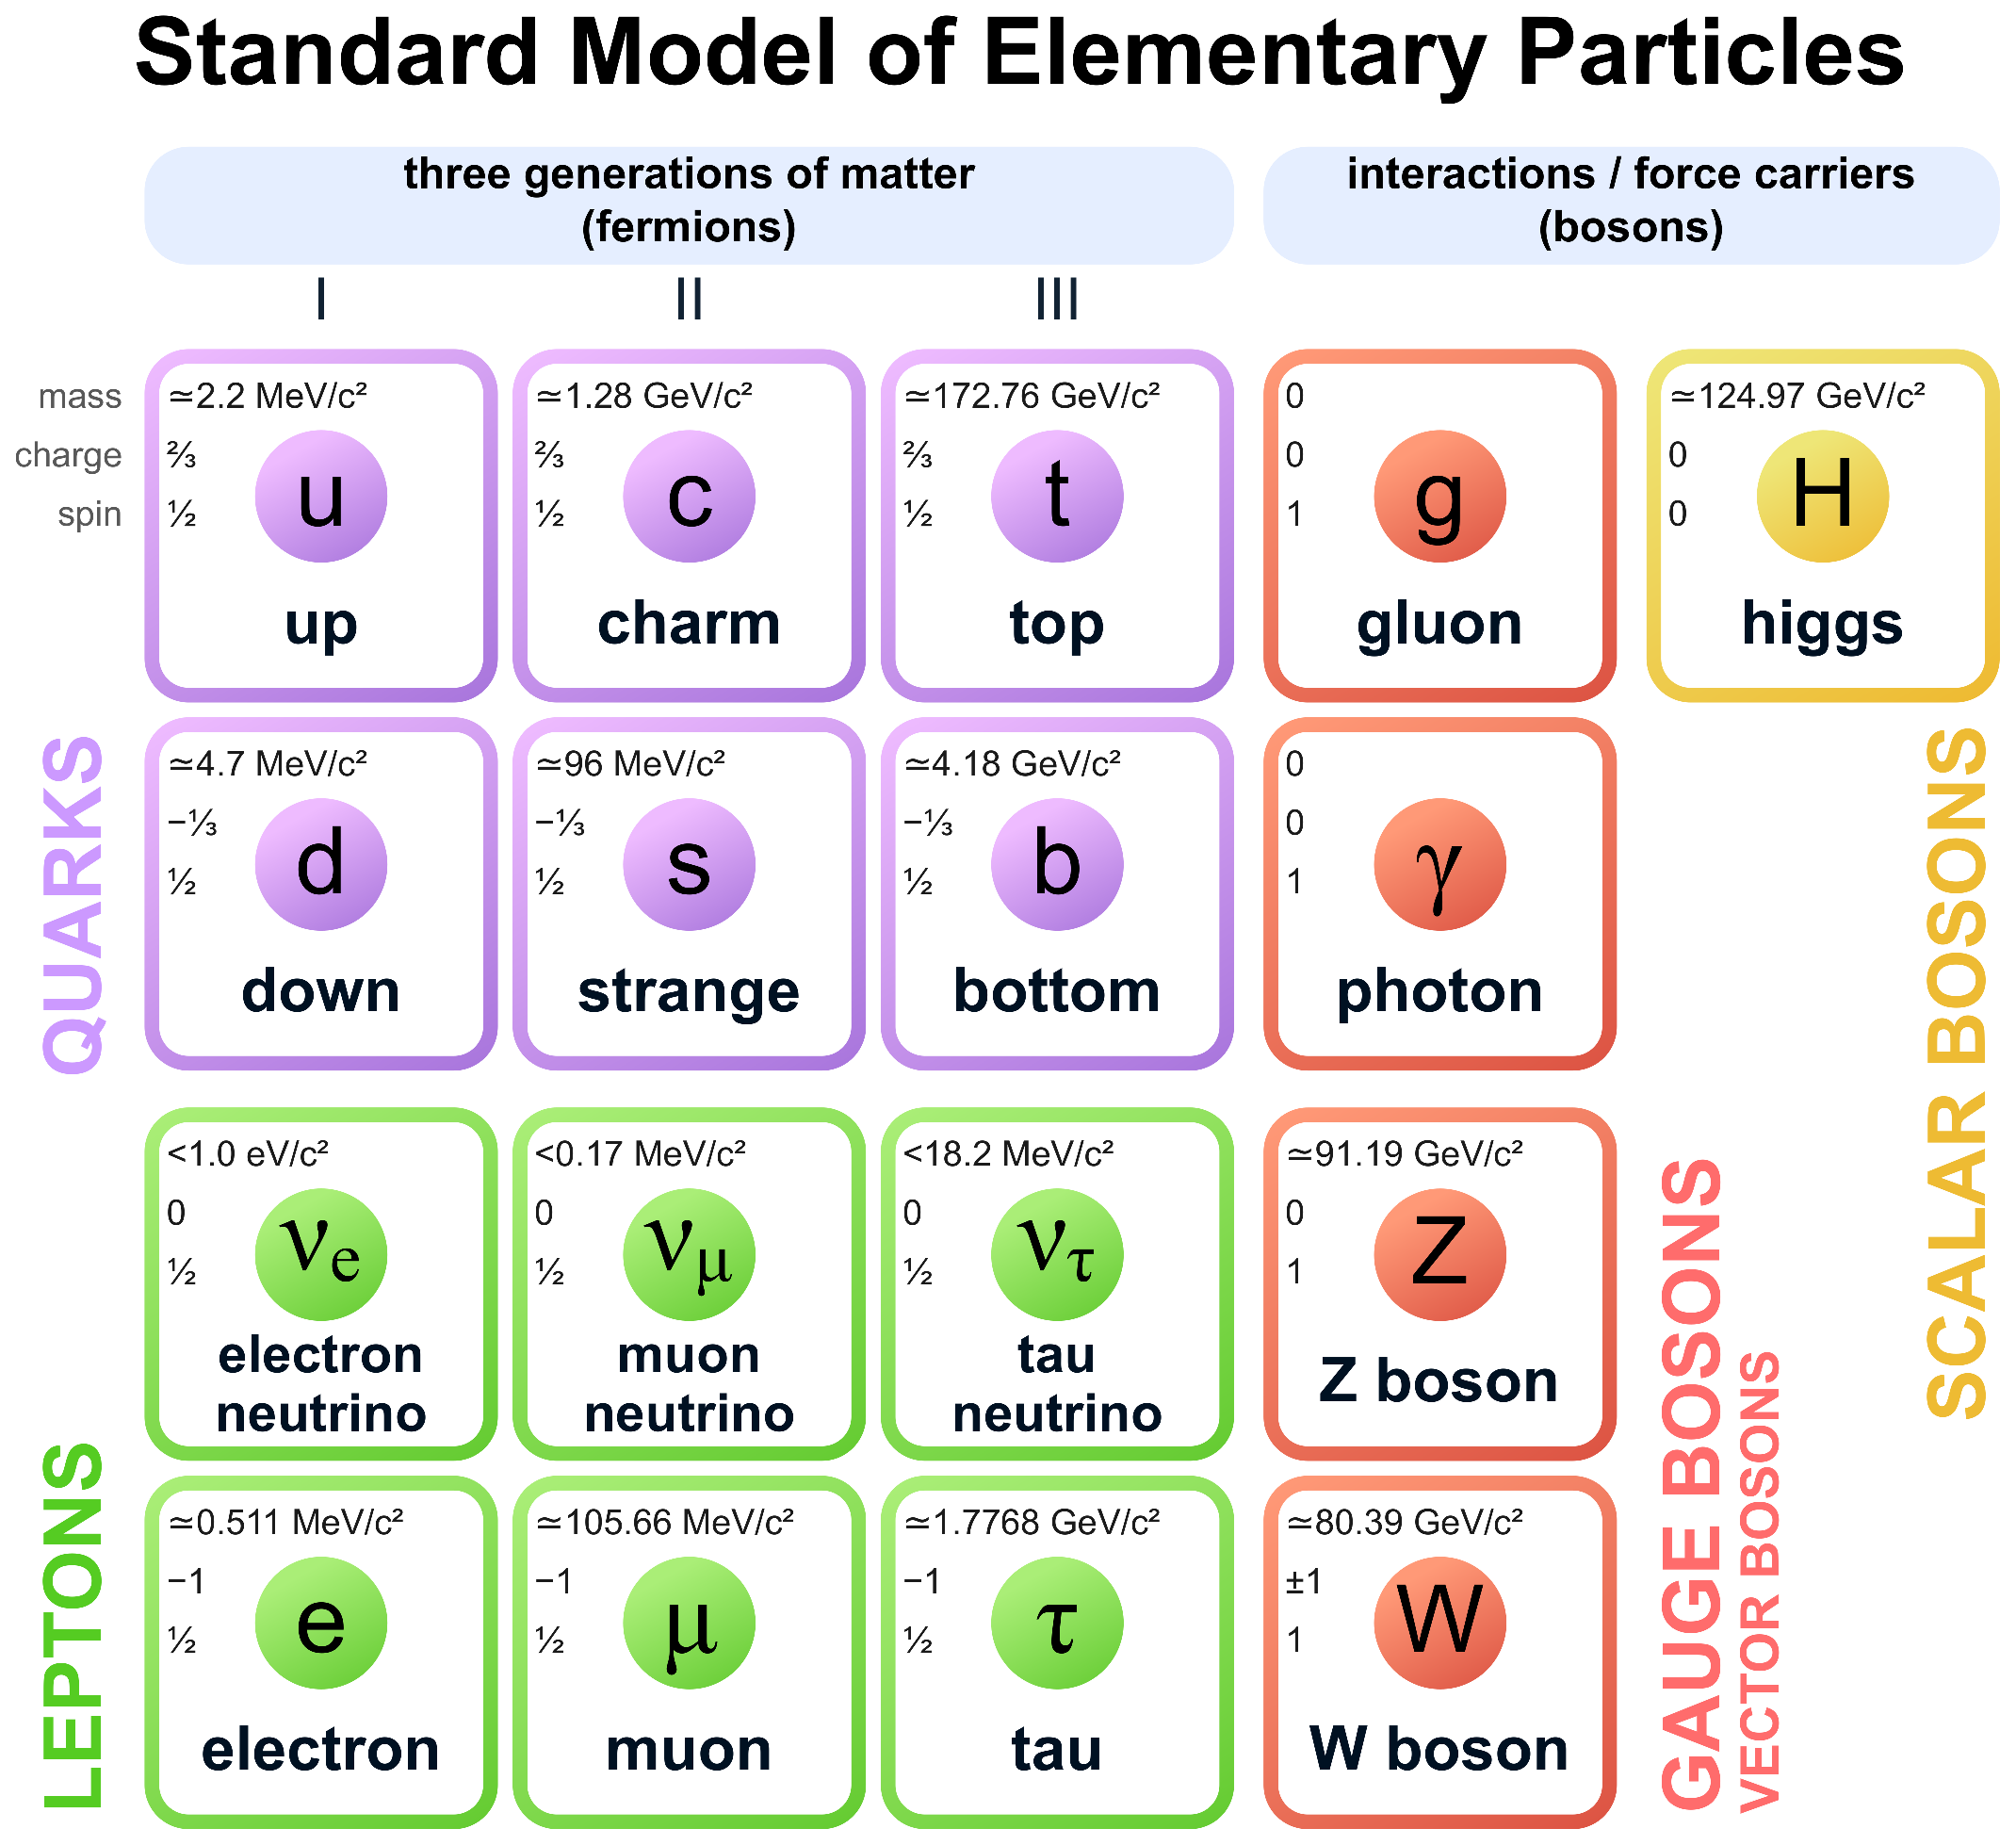
\includegraphics[width=.75\textwidth]{figures/theory/standard_model.eps}
	\caption{The elementary particles of the Standard Model subdivided into fermions (left) and bosons (right). The fermions are further split into quarks (top) and leptons (bottom), which are each divided into three generations. The bosons are divided into four vector bosons and one scalar boson.}
	\label{fig:standard_model}
\end{figure}

\section{The Top Quark}
The top ($t$) quark was discovered in 1995 at \fermilab by the experiments \cdf\cite{top_production01} and \dzero \cite{top_production02}. It is assumed to be the partner of the bottom ($b$) quark with a mass of $m_t=172.76\pm0.30,\text{GeV}$ \cite{top_mass}, which makes it the heaviest of all known quarks and has a very short lifetime of $\tau_t\approx5\cdot10^{-25}\,\text{s}$ \cite{top_mass}. The \tquark decays via the weak interaction into a \wboson and a down-type quark before it hadronises. The probability of decaying into a particular down-type quark is given by the respective CKM-matrix element \cite{ckm_matrix}. Due to the CKM-matrix having vanishing off-diagonal contributions, \tquarks predominantly decay into \bquarks. The \wboson further decays either into a charged lepton and neutrino, which results in one jet from the \bquark and one measurable lepton, or into a quark-antiquark-pair which results in three produced jets.
%
%\begin{table}[t]
%	\renewcommand{\arraystretch}{1.5}
%	\centering
%	\begin{tabular}{R{40mm}C{60mm}C{10mm}C{10mm}}
%		Signal	& Reaction & Jets & Leptons\\
%		\hline
%		Lepton 		& $t\rightarrow bW^+ \rightarrow b(\bar{l}\nu_l)$ & 1 & 1(+1)\\
%		Jets		& $t\rightarrow bW^+ \rightarrow b(q\bar{q'})$ 	& 3 & 0\\
%	\end{tabular}
%	\caption{Possible signals from the \wboson decay modes. The number of leptons in brackets corresponds to the number of neutrinos.}
%	\label{tab:decay_modes_t}
%\end{table}

Producing \tquarks requires high energies due to the mass of the \tquark. These energies can be achieved in hadrons colliders. Figure~\ref{fig:production_ttz_ttw} shows two example processes for \tquark production in \ttbar-processes. Each of the two \tquarks decays as described before, therefore the measured signal depends on the \wboson decay mode.

\section{\ttbar{} Production in Association with a $Z$/$W$-Boson}
\label{sec:theory_ttZ_ttW}
When producing \ttbar pairs, an additional \zwboson can be produced. Figure~\ref{fig:production_ttz_ttw} shows example processes for \ttbar-production via gluon-gluon fusion and quark-antiquark annihilation with an additional \zwboson. Since the \lhc is a proton-proton collider, the gluon-gluon fusion process is dominating. A selection of possible signals from \ttbarZ/\ttbarW events is summarised in Table~\ref{tab:decay_modes_ttz_ttW}.

The \ttbarZ events are of interest as they allow studying the coupling of \tquarks to neutral currents of the weak interaction through final state radiation of a \zboson in \ttbar events. Therefore, \ttbarZ events allow analysing the third component of the weak isospin of \tquarks.

The \ttbarW events are not sensitive to the coupling of \tquarks to charged currents of the weak interaction, because, as seen in Fig~\ref{fig:production_ttz_ttw}, the \wbosons are only emitted as initial state radiation. However, the \ttbarW processes are sensitive to the initial parton distribution functions (PDF) and thus measurements on these processes probe those PDFs.

Analysing \ttbarZ/\ttbarW events together at the same time is particularly interesting because both can generate similar signals and thus are important background processes for each other. Especially studying these events in off-shell regions gives rise to a high rate of background from the respective other process. Some kinematic variables in \ttbarZ/\ttbarW off-shell events like invariant mass and transverse momentum   are also expected to be sensitive to SM-EFT contributions. Furthermore, the sensitivity of these SM-EFT contributions is expected to increase for higher boson masses \cite{sm_eft_top}.

\begin{figure}[t]
	\centering
	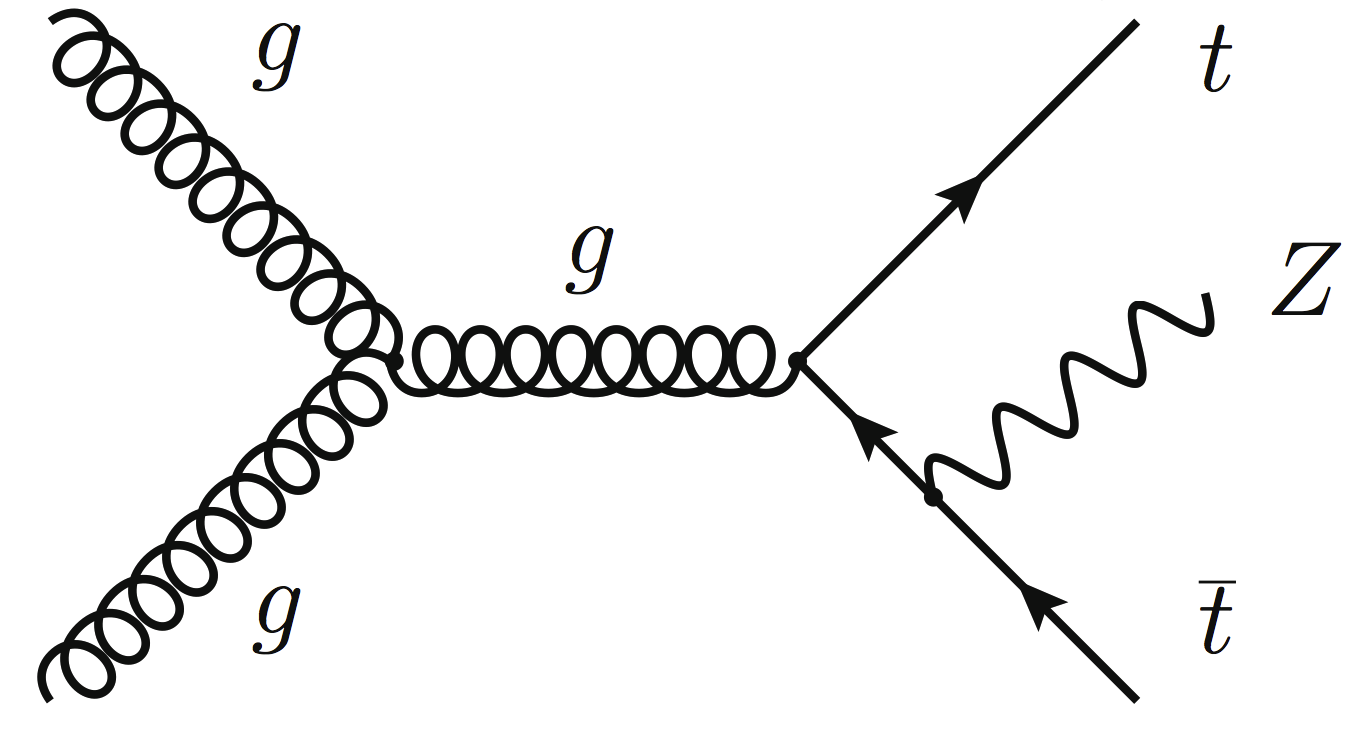
\includegraphics[width=.4\textwidth]{figures/theory/ttZ_feynman.png}\hspace{.1\textwidth}
	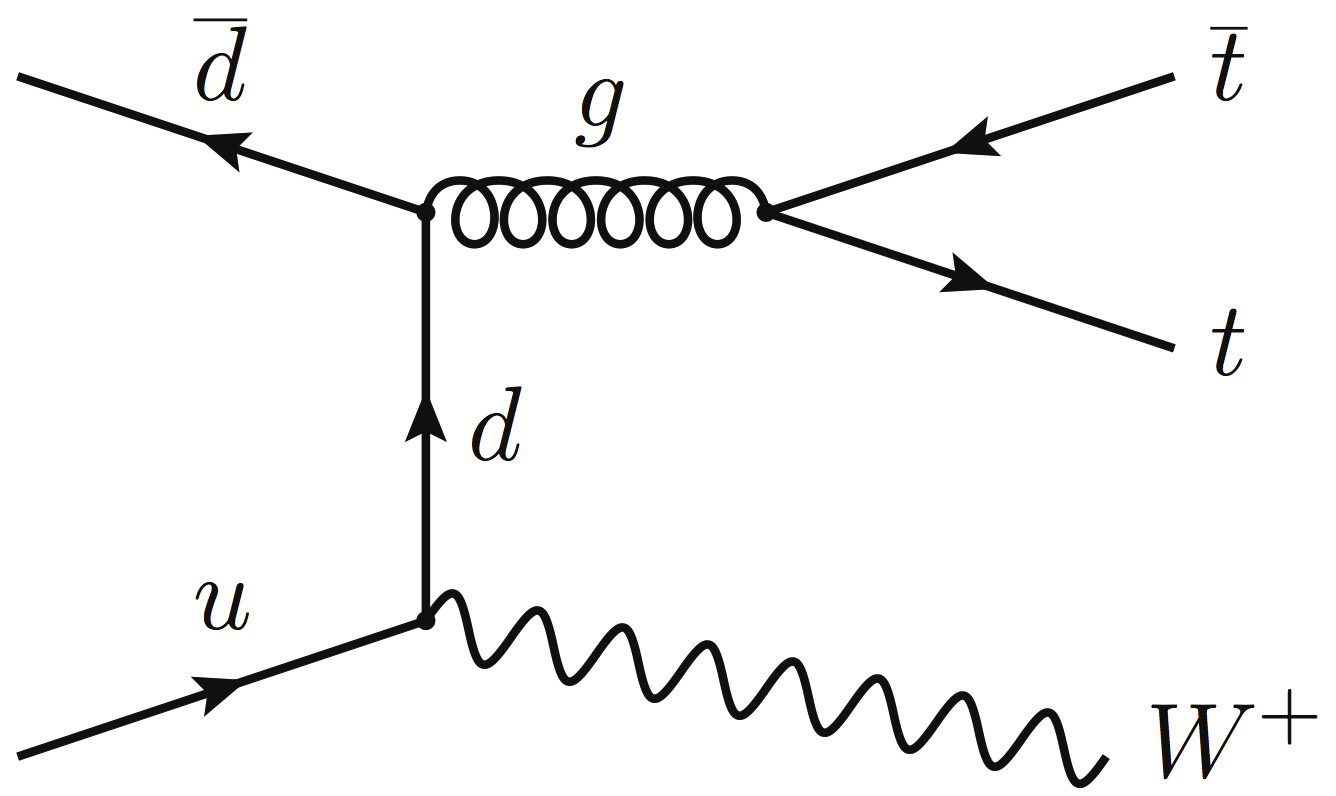
\includegraphics[width=.4\textwidth]{figures/theory/ttW_feynman.png}
	\caption{The Feynman diagrams for an example \ttbarZ process by gluon-gluon fusion (left) in which the produced \ttbar pair emits an additional \zboson and a \ttbarW process by quark-antiquark annihilation (right) emitting the \wboson as initial state radiation.}
	\label{fig:production_ttz_ttw}
\end{figure}

\begin{table}[t]
	\renewcommand{\arraystretch}{1.5}
	\centering
	\caption{Possible leptonic signals from \ttbarZ/\ttbarW events which provides a cleaner measurement in comparison to the hadronic decays. At least one of the \tquarks or the \zwboson decays into leptons. The number in brackets shows the number of not measurable neutrinos.}
	\begin{tabular}{R{40mm}C{1mm}L{50mm}C{10mm}C{15mm}}
		Signal	&& Reaction & Jets & Leptons\\
		\hline
		\ttbarW-Monoleptonic 	&& $t\bar{t}W\rightarrow(bq\bar{q}')\,(\bar{b}q\bar{q}')\,(\ell\bar{\nu_\ell})$ 			& 6 & 1(+1)\\
		\ttbarW-Dileptonic 		&& $t\bar{t}W\rightarrow(bq\bar{q}')\,(\bar{b}\ell\bar{\nu_\ell})\,(\ell\bar{\nu_\ell})$ 	& 4 & 2(+2)\\
		\ttbarW-Trileptonic 	&& $t\bar{t}W\rightarrow(b\bar{\ell}\nu_\ell)\,(\bar{b}\ell\bar{\nu_\ell})\,(\ell\bar{\nu_\ell})$ & 2 & 3(+3)\\
		\ttbarZ-Dileptonic 		&& $t\bar{t}Z\rightarrow(bq\bar{q}')\,(\bar{b}q\bar{q}')\,(\ell\bar{\ell})$ 				& 6 & 2(+0)\\
		\ttbarZ-Trileptonic 	&& $t\bar{t}Z\rightarrow(bq\bar{q}')\,(\bar{b}\ell\bar{\nu_\ell})\,(\ell\bar{\ell})$ 		& 4 & 3(+1)\\
		\ttbarZ-Tetraleptonic 	&& $t\bar{t}Z\rightarrow(b\bar{\ell}\nu_\ell)\,(\bar{b}\ell\bar{\nu_\ell})\,(\ell\bar{\ell})$ 	& 2 & 4(+2)\\
	\end{tabular}
	\label{tab:decay_modes_ttz_ttW}
\end{table}

\section{Effective Field Theory}
\label{sec:TheoryEFT}
For the analysis of effects beyond the Standard Model, one can use an Effective Field Theory (EFT) approach such as the Standard-Model Effective Field Theory (SM-EFT) \cite{eft_operatorlist}. This theory assumes that the current SM is an effective low-energy approximation which holds for interactions up to an energy scale $\Lambda$ and can be expanded using higher dimensional interactions \cite{eft_introduction}. The transition into the Standard Model happens via decoupling of heavy particles at energies higher than $\Lambda$. Therefore, higher-dimensional operators $Q$, which are suppressed by powers of $\Lambda$, are used in a perturbation expansion \cite{eft_introduction}
\begin{align}
	\mathcal{L}_\text{SM-EFT} = \mathcal{L}_\text{SM} + \frac{1}{\Lambda}\sum_{k}C_k^{(5)}Q_k^{(5)} + \frac{1}{\Lambda^2}\sum_{k}C_k^{(6)}Q_k^{(6)} + \mathcal{O}\left(\frac{1}{\Lambda^3}\right)\;.\label{eq:SM-EFT}
\end{align}
In this perturbation expansion $\mathcal{L}_\text{SM}$ describes the common SM-Lagrangian, $Q_k^{(n)}$ the $n$-dimensional interaction operators and $C_k^{(n)}$ their corresponding Wilson coefficients. 

For a better understanding of \ttbarZ and \ttbarW production, their relevant operators can be analysed. Since the \zboson is a combination of the $W^0$- and $B$-bosons originating the Brout-Englert-Higgs mechanism, the operator \optZ for the $tZ$-coupling is given by \cite{higgs_mechanism_1}
\begin{align}
	Q_\text{tZ} &= \cos(\Theta_W)Q_\text{tW} - \sin(\Theta_W)Q_\text{tB}\;.\label{eq:OparatortZ}
\end{align}
Hence, the operators for the $tW$- and the $tB$-coupling and their complex coefficients \ctW and \ctB are of particular interest for this analysis \cite{eft_operatorlist}. To measure the sensitivity, the separation power 
\begin{align}
	S &= \frac{1}{2}\sum_\text{Bins}\frac{\left(\text{EFT}_i-\text{SM}_i\right)^2}{\text{EFT}_i+\text{SM}_i}\label{eq:SeparationPower}
\end{align}
is used. The fraction inside the sum is calculated for each bin for a given normalised distribution. $\text{SM}$ stands for the Standard Model prediction and $\text{EFT}$ includes a specific variation on one or multiple Wilson coefficients as in Equation~\ref{eq:SM-EFT}. Studies regarding the sensitivity of several variables for these coefficients are summarised in Chapter~\ref{ch:eft_sensitivity}. 


\chapter{Experimental Setup}
\label{ch:experimental_setup}
For collecting data of \ttbarZ and \ttbarW events, a high energy particle collider is needed. Furthermore, a setup for the detection of signals as well as appropriate reconstruction algorithms are necessary.

The 27\,km long Large Hadron Collider (\lhc) is a proton-proton collider. The centre-of-mass energy reached by the \lhc was around 7-8\,TeV during Run~I and 13\,TeV during Run~II \cite{lhc2}. During Run~III the centre-of-mass energy is expected to reach 13.6\,TeV \cite{lhc_run3}. Those high-energy collisions produce multiple particles like \tquarks, which in turn decay into more particles. Detecting events requires a calibrated detector system which measures the properties of the particles such as charge, momentum and energy. Furthermore, the event reconstruction from measured signals uses several algorithms to reconstruct for example the particles trajectories and collision vertices.

The \atlas-detector \cite{atlas} is a multi-purpose particle detector that consists of different layers for detecting various particles. These layers are built in concentric cylinders around the beam axis. Measurements of the tracks and deposited energies of the decay products allow the reconstruction of the initial particles. Figure~\ref{fig:atlas} shows a schematic view of those detector layers. Each layer is described in the following. 

\begin{figure}[t]
	\centering
	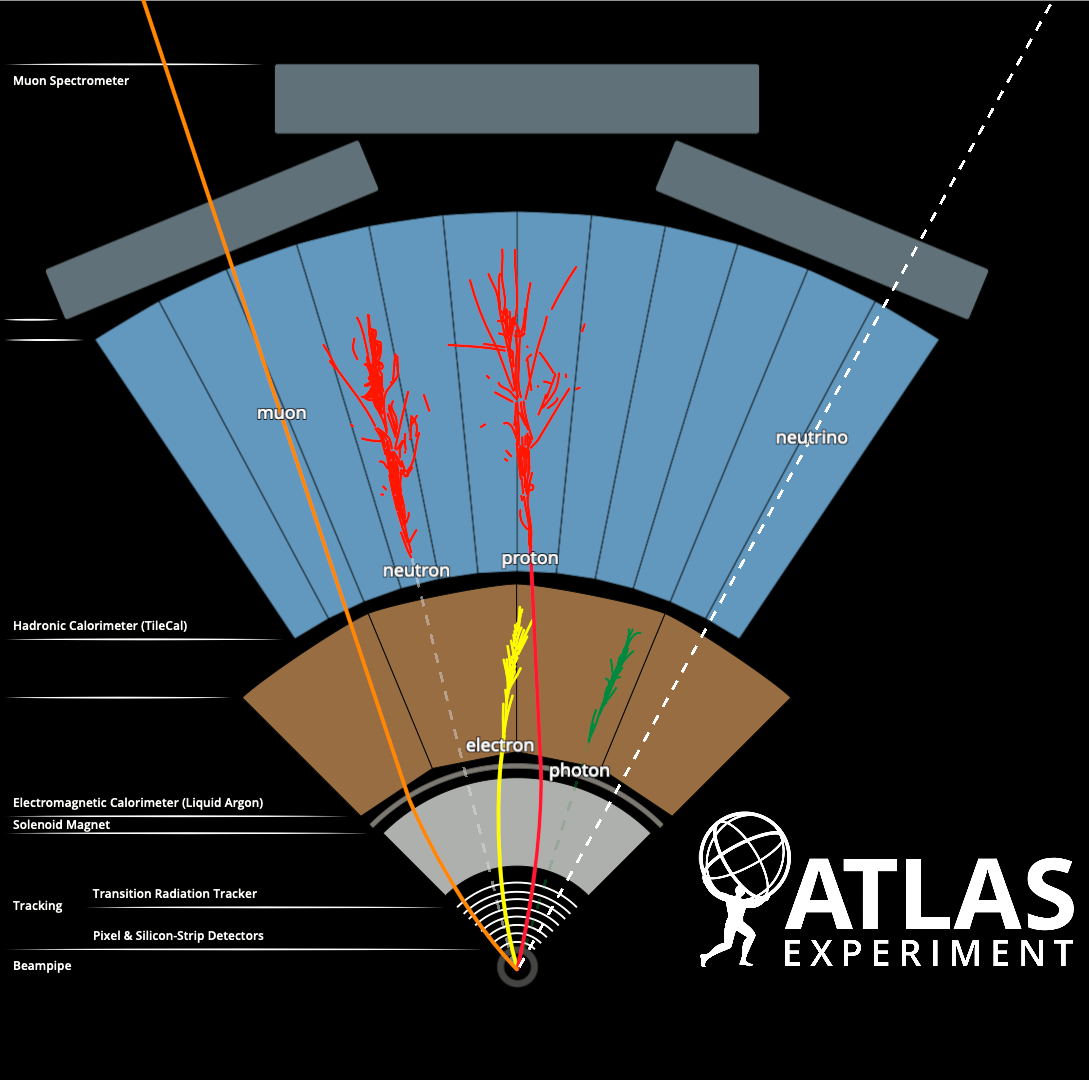
\includegraphics[width=.61\textwidth]{figures/atlas/atlas3.png}
	\caption{Cross-section of the concentric layers inside the \atlas Detector (\copyright{} \cern).}
	\label{fig:atlas}
\end{figure}

\section*{The Inner Detector}
The task of the Inner Detector is to precisely measure the tracks of various charged particles. Because of the 2\,T magnetic field, which is induced by a central solenoid, the moving charged particles are deflected via the Lorentz force. Measurements of the curvature allows precise measurements of their momentum and reconstructing the particle track. Thus, the tracking system is crucial for $b$-tagging because it makes it possible to identify secondary vertices, which are indications for $b$-jets \cite{atlas}. Because of the high density of particles in the detector close to the collision point, high-precision measurements use Pixel-, Strip- and Transition Radiation Trackers.

The Pixel Tracker is the first point of detection and allows tracking near the collision point using small Pixel-modules \cite{atlas}. It is built from silicon to withstand strong radiation from the collision. The semiconductor Strip Tracker (SCT) consists of longer strips that also contribute to the tracking by offering larger scale measurement.

The Transition Radiation Tracker (TRT) is built from thin and long polyimide straws \cite{atlas}. These straw tubes are filled with a gas mixture and while they offer a worse resolution, they allow for a relatively cheap way to cover a greater volume and hence, contribute to a precise measurement. It is used to distinguish electrons $e^\pm$ and charged pions $\pi^\pm$.

\section*{The Calorimeters}
As seen in Figure~\ref{fig:atlas}, the calorimeters are built around the Inner Detector and the solenoid magnet. In general, the calorimeters measure the energy of particles by stopping them. The calorimeter system used in the \atlas-detector is subdivided into the electromagnetic and the hadronic calorimeter. Both are sampling calorimeters that have an absorber material, which induces particle showers and an active medium, which is used for measuring the signals \cite{atlas_calorimeter}.

The electromagnetic calorimeter measures all particles that interact electromagnetically. Those charged particles and photons each create an electromagnetic shower which can be used to reconstruct the initial particles. It offers a precise measurement of the deposited energy and the location of the energy-deposition. It is built from Lead as the absorber and liquid Argon as active medium \cite{atlas_calorimeter}.

The hadronic calorimeter absorbs particles that pass the electromagnetic calorimeter and interact via the strong force. The hadronic showers created can produce additional electromagnetic sub-showers which makes them more difficult to reconstruct and less precise. It consist of steel as an absorber and plastic scintillating tiles \cite{atlas_calorimeter}.

\section*{The Muon Spectrometer}
The Muon Spectrometer is the outermost layer and follows a similar approach as the Inner Detector to measure the momentum of muons which usually pass the Inner Detector and Calorimeter undetected. It consists of four different subsystems \cite{atlas}. 

For the muon triggering, the Resistive Plate Chambers (RPC) and Thin Gap Chambers (TGC) are used in different regions of the detector. Furthermore, they are used in the coordinate measurement. The Cathode Strip Chambers (CSC) offer a more precise coordinate measurements at the ends of the detector. Lastly, the Monitored Drift Tubes (MDT) track the curved trajectories of the muons. The magnetic field responsible for deflecting the muons is generated by outer toroidal magnets \cite{atlas}.


\chapter{Region Definition}
\label{ch:region_definition}
This investigation of simultaneous measurements utilises the trileptonic decay channel because of its cleaner event signature in comparison to hadronic or single leptonic decays. Sensitive regions for \ttbarZ and \ttbarW are defined to be used in fitting process. Since the trileptonic channel is used, non-prompt electrons (fakes) are also a dominant background. Thus, ideally a signal region for \ttbarZ and two separate control regions for \ttbarW and fakes are defined.

\section{Preselection}
\label{sec:preselection}
The analysis only includes events with exactly three electrons or muons, three or more jets of which at least one needs to be $b$-tagged and an off-shell \zboson in the final state. A \zboson is labelled as off-shell if the reconstructed mass differs from the SM prediction by at least 10\,GeV. Because of the low statistics in the off-shell region, the 85\% working point for $b$-tagging is chosen. Additionally, these events need to have a lepton pair of opposite sign and same flavour (OSSF) which is expected to originate from the \zboson. This OSSF-pair is required to have a reconstructed mass of at least 10\,GeV to suppress background contributions from low-mass resonances. All three leptons have to pass the tight selection and need to satisfy $p_\text{T,1}\geq27\,\unit{GeV}$, $p_\text{T,2}\geq20\,\unit{GeV}$ and $p_\text{T,3}\geq15\,\unit{GeV}$ respectively. These preselections are applied to all events before region definition. For the binning of variables, the same algorithm as described in Section 5.3.1 of Reference~\cite{algorithm_transfod} is used and was tested for several numbers of bins of which 6 bins were found to be optimal.

%\begin{table}
%	\centering
%	\caption{The preselection for the off-shell \ttbarZ, \ttbarW analysis in the trileptonic channel.}
%	\begin{tabular}{l|l}
%		Variable						& Selection\\
%		\hline
%		Number of Jets 					& $\geq3$\\
%		$b$-tagged Jets (at 85\% WP)	& $\geq1$\\
%		Has OSSF-pair 					& True\\	
%		$m_\text{OSSF}$ 				& $\geq10$\,GeV\\
%		& $|m_\text{OSSF}-m_\text{Z}^\text{SM}|\geq10$\,GeV\\
%		nEl + nMu						& $=3$\\
%		Leptons pass tight selection 	& True\\
%		Lepton \pT						& $\geq(27,20,15)$\,GeV\\	
%		%		$m_\text{Z}$ 					& $<81.1876$\,GeV or $>101.1876$\,GeV
%	\end{tabular}
%	\label{tab:preselection}
%\end{table}

\section{Cut And Count Based Region Definition}
\label{sec:CountAndCountBasedRegionDefinition}
To define sensitive regions, several cuts on kinematic variables are analysed. The choice of variables is motivated by the underlying physical processes as described in Section~\ref{sec:theory_ttZ_ttW}. 

The best performance was achieved by using the missing energy \ETMiss and the $\Delta R$ variable which is defined as
\begin{align}
	\Delta R &= \sqrt{\left(\Delta\phi\right)^2+\left(\Delta\eta\right)^2}
\end{align}
between two objects. \dR between the OSSF-pair is of particular interest. The reason for that is that the leptons from the \zboson decay in \ttbarZ events are expected to be more bundled and hence closer in $\Delta R$ compared to other lepton combinations. Also, \ttbarW should have higher values for \ETMiss than \ttbarZ, since \ttbarW processes have three neutrinos in their final state instead of only one for \ttbarZ events. Furthermore, these two variables offer fine region tuning, since they are continuously distributed unlike for example jet multiplicities. 

The cuts are set by evaluating the separation plots in Figure~\ref{fig:InitialSeparationPlotsETMissdR} and choosing the initial cut-off at the values for which the \ttbarW background becomes larger than the \ttbarZ signal. Several configurations were tested by varying those cuts. A lower cut value for \ETMiss and a higher value for \dR were found to have the best performance. These can also be seen in Figure~\ref{fig:InitialSeparationPlotsETMissdR}. The cut and count (CC) based region definition is summarised in Table~\ref{tab:Regions} and the corresponding yields can be found in Table~\ref{tab:Yields}.

\begin{table}
	\centering
	\caption{The selections for the (top) cut and count based and (bottom) neural network based region definition.}
	\vspace{1mm}
	\begin{tabular}{lVl}
		Region 			& Selection\\
		\hline
		SR-ttZ-CC 			& \dR$<1.8$\\
		CR-ttW-CC 			& \dR$\geq1.8$; \ETMiss$\geq78\,\unit{GeV}$\\
		CR-Fakes-CC 		& \dR$\geq1.8$; \ETMiss$<78\,\unit{GeV}$\\
		\hline
		SR-ttZ-NN 			& ttW score$<0.4$, Fakes score$<0.4$\\
		CR-ttW-NN 			& ttW score$\geq0.4$\\
		CR-Fakes-NN 		& ttW score$<0.4$, Fakes score$\geq0.4$\\
	\end{tabular}
	\label{tab:Regions}
\end{table}

\begin{figure}
	\centering
	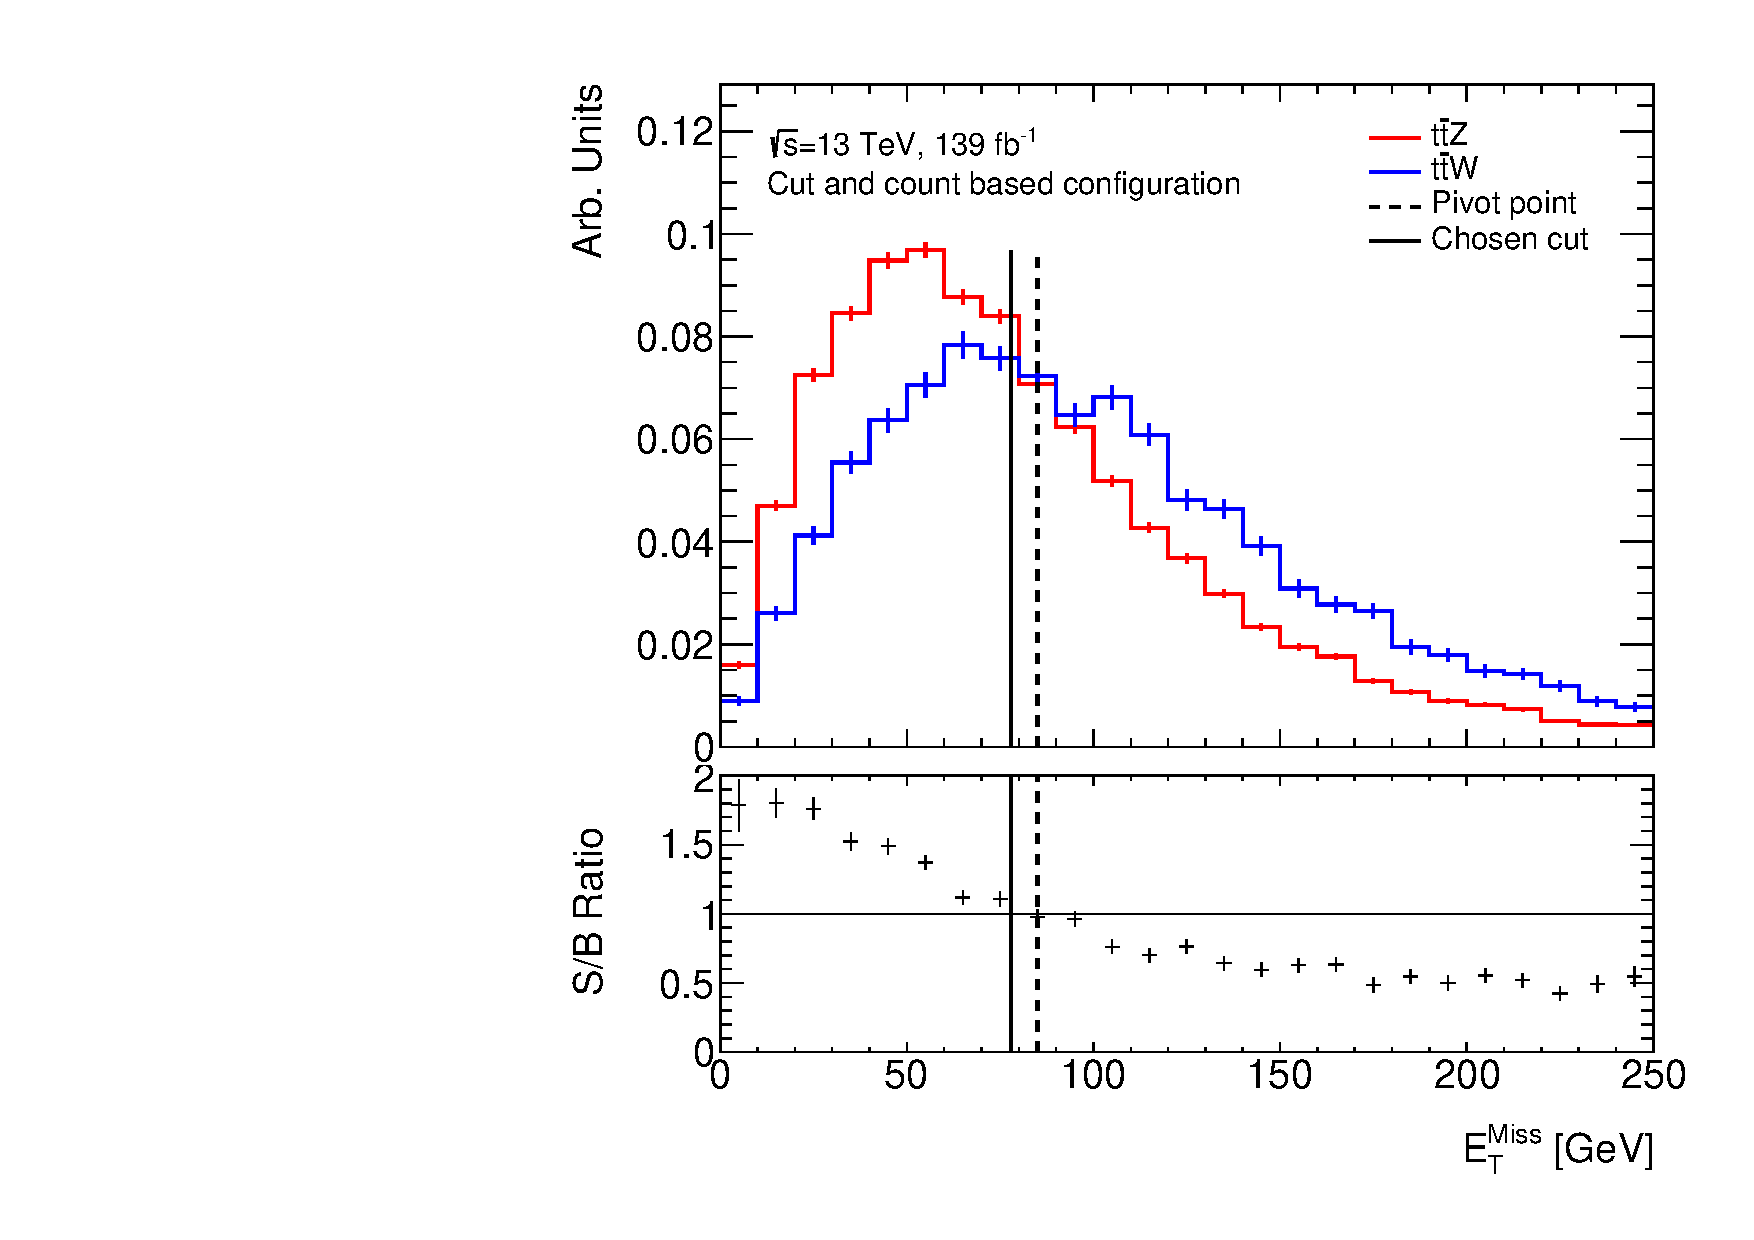
\includegraphics[width=.4\textwidth]{initial_config/separation/_hiZ_sep_eT_miss.pdf}\hspace{8mm}
	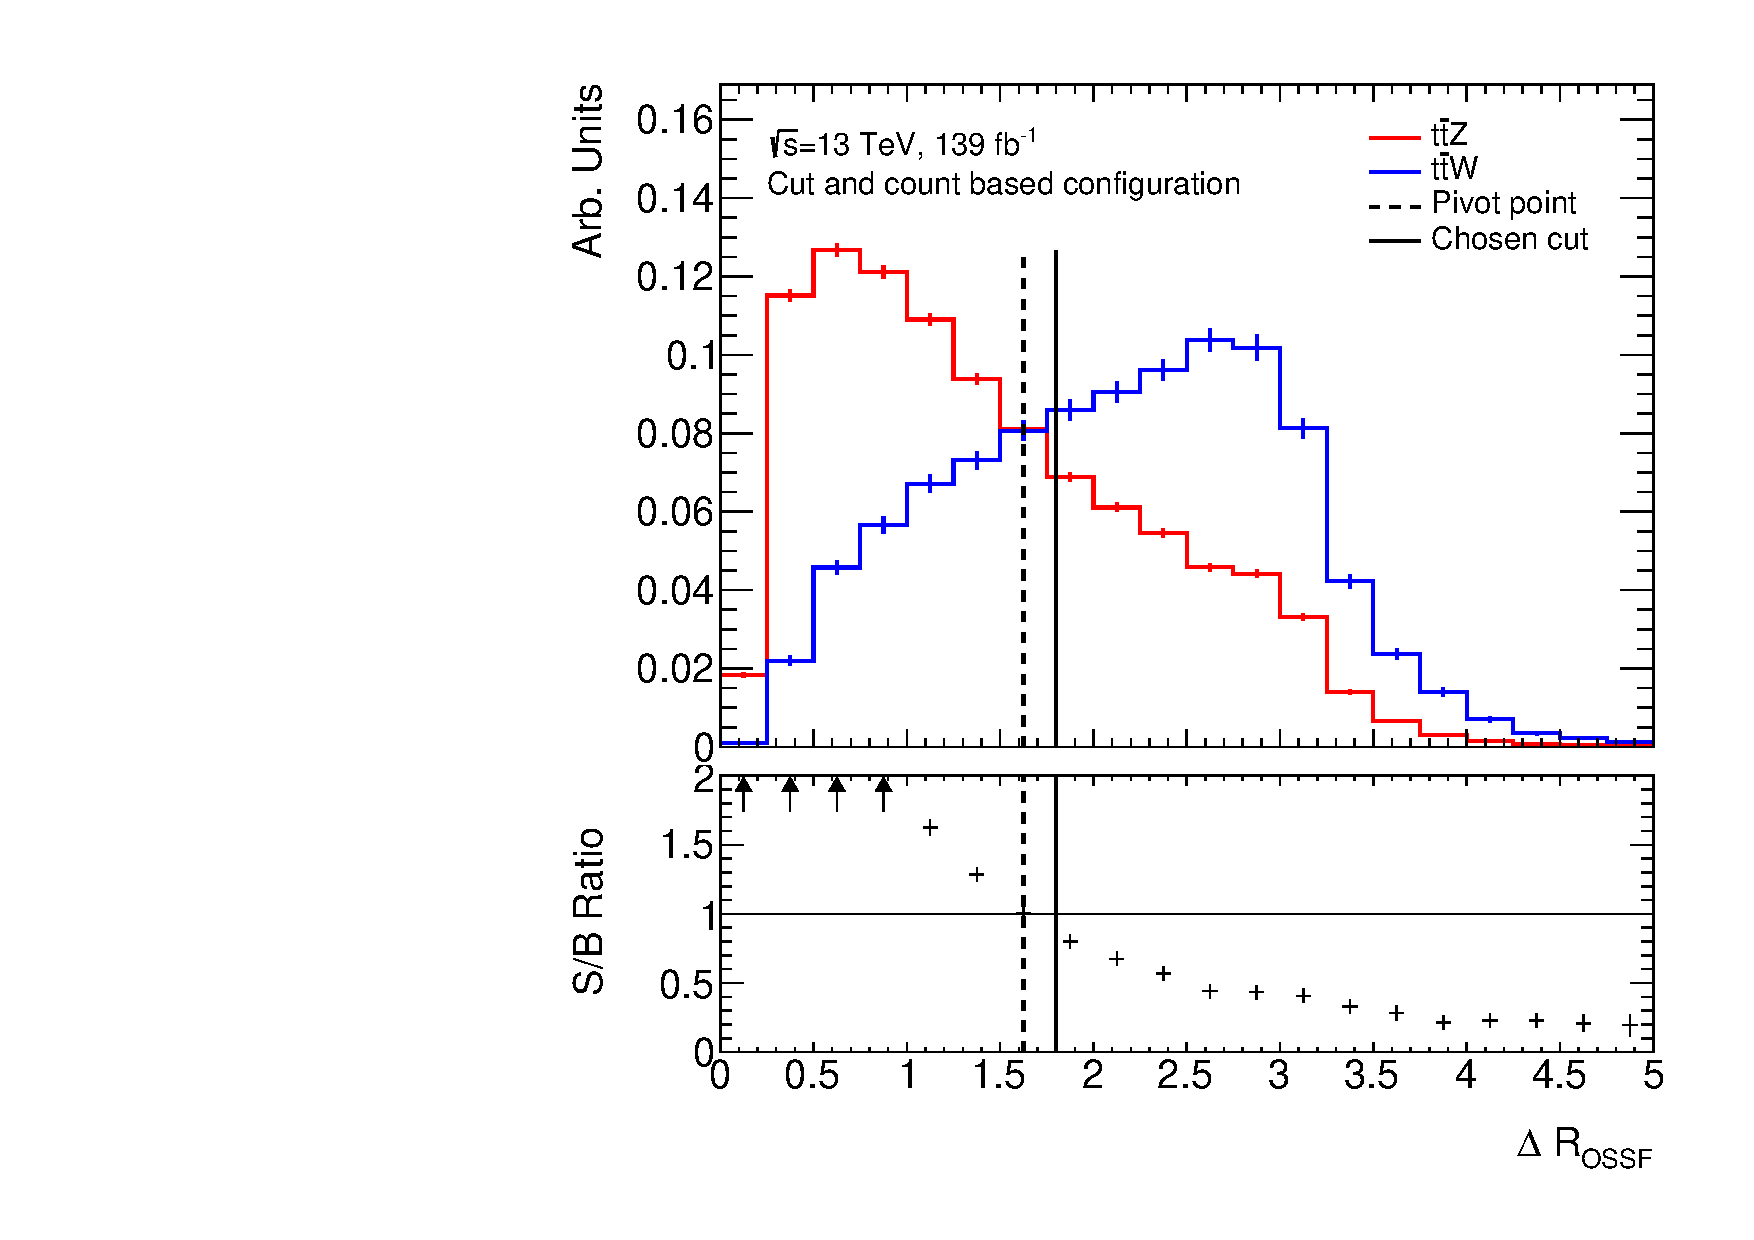
\includegraphics[width=.4\textwidth]{initial_config/separation/_hiZ_sep_dRllz1_dR.pdf}
	\caption{The separation plots for \ETMiss (left) and \dR (right) used in the cut and count based configuration. The dashed lines represent the point at which the \ttbarW background becomes higher than the \ttbarZ signal. The solid line shows the chosen cut for the best performance.}
	\label{fig:InitialSeparationPlotsETMissdR}
\end{figure}


\section{Neural Network Based Region Definition}
\label{sec:NeuralNetworkBasedRegionDefinition}
To improve the quality of the defined regions, a neural network is implemented. Its task is to define three classes, each corresponding to either \ttbarZ, \ttbarW or fakes events. The class scores are based on several input variables which are expected to be sensitive to these processes. The architecture of the neural network and the used input variables are further explained in Section~\ref{sec:NeuralNetworkArchitecture}. 

For the placement of the class score cuts, the 2D separation plots in Figure~\ref{fig:Final2DSeparationPlots} are used. These plots show the two dimensional projection of the event distribution in respect to the three class scores. Since the neural network uses the \textit{Softmax} activation for the output layer, the sum of all class scores are normalised to one. Thus, all events lie on a three dimensional plane. Two linear cuts were chosen to separate \ttbarW and fakes from the \ttbarZ events. Figure~\ref{fig:Final2DSeparationPlots} also shows these cut placements.

The neural network (NN) based region definition is also summarised in Table~\ref{tab:Regions} and the corresponding yields are listed in Table~\ref{tab:Yields}.

%\begin{table}
%	\centering	
%	\caption{The neural network based region definition using the class score. The SR is expected to be sensitive to \ttbarZ signals and the two CR should have high contributions from \ttbarW and Fakes respectively.}
%	\begin{tabular}{lVll}
%		Region 				& Selection\\
%		\hline
%		SR-offZ-ttZ 		& \ttbarW score$<0.4$, Fakes score$<0.4$\\
%		CR-offZ-ttW 		& \ttbarW score$\geq0.4$\\
%		CR-offZ-Fakes 		& \ttbarW score$<0.4$, Fakes score$\geq0.4$\\
%	\end{tabular}
%	\label{tab:FinalRegions}
%\end{table}


\begin{figure}
	\centering
	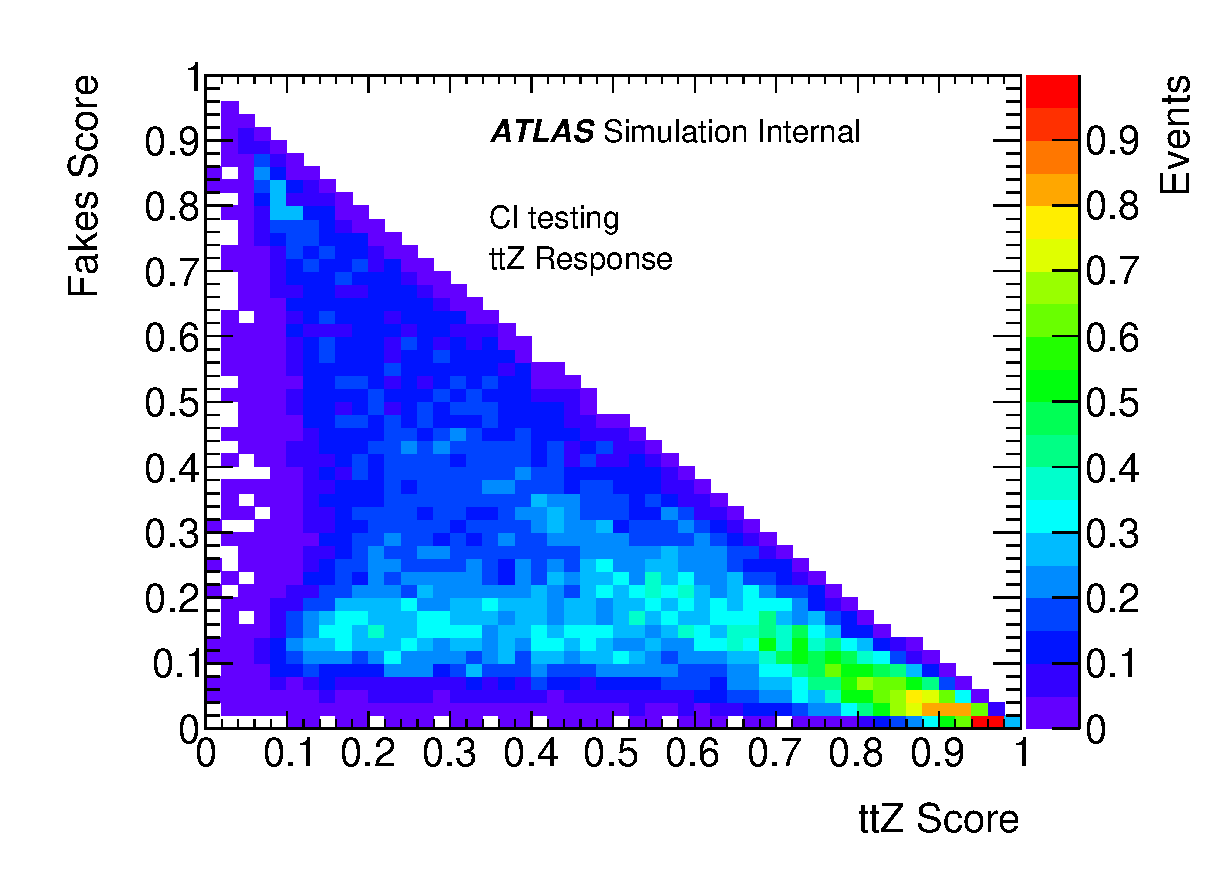
\includegraphics[width=.4\textwidth]{final_config/2d_mva/MyModel_ttZ_2DMVA.eps}\hspace{8mm}
	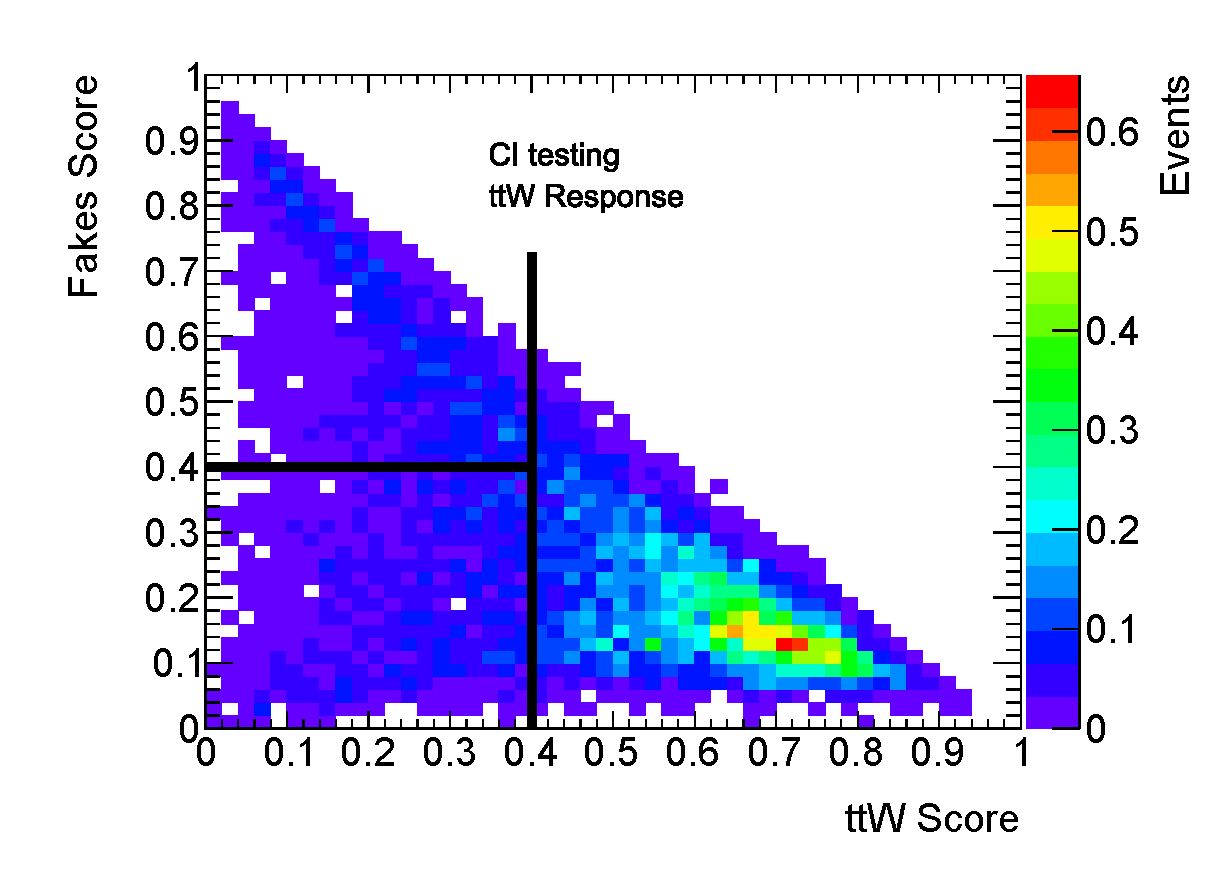
\includegraphics[width=.4\textwidth]{final_config/2d_mva/MyModel_ttW_2DMVA.eps}
	
	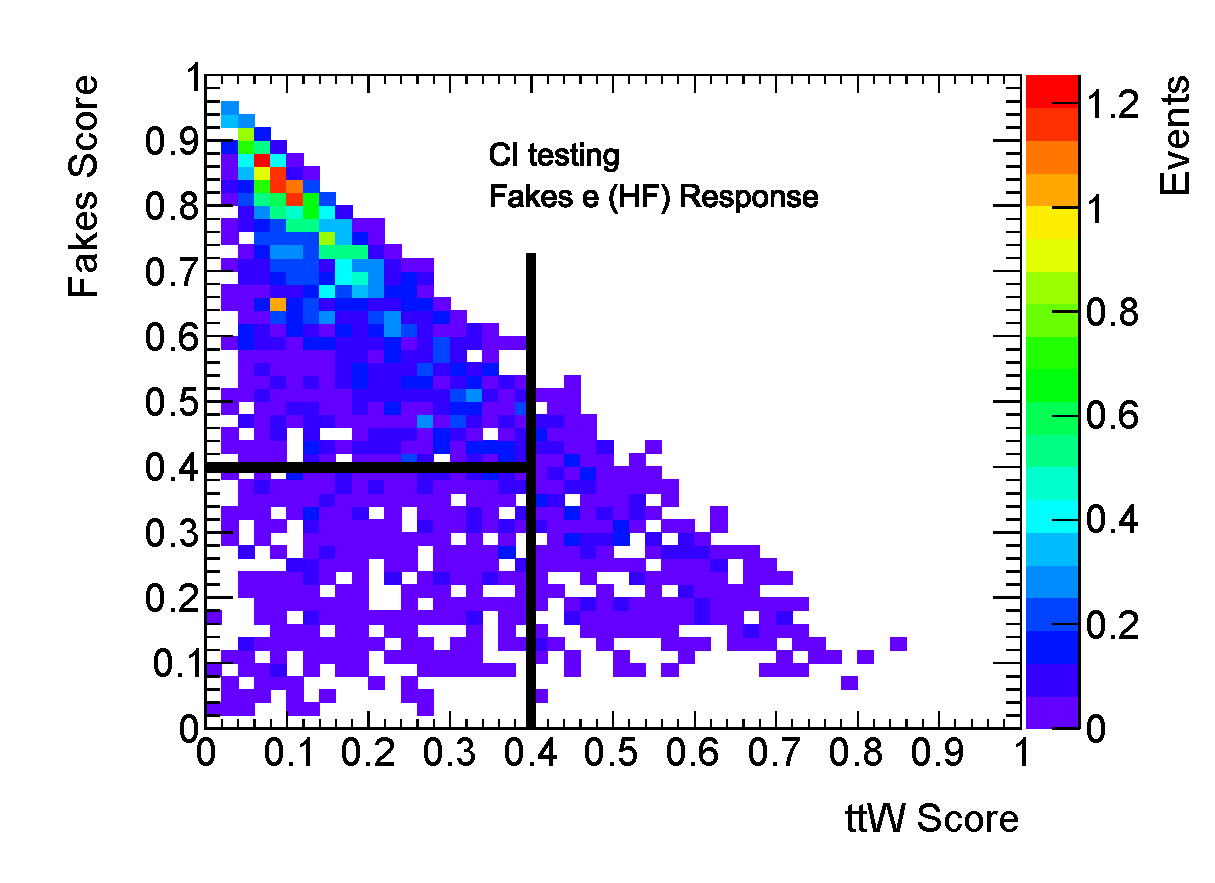
\includegraphics[width=.4\textwidth]{final_config/2d_mva/MyModel_Fakese(HF)_2DMVA.eps}\hspace{8mm}
	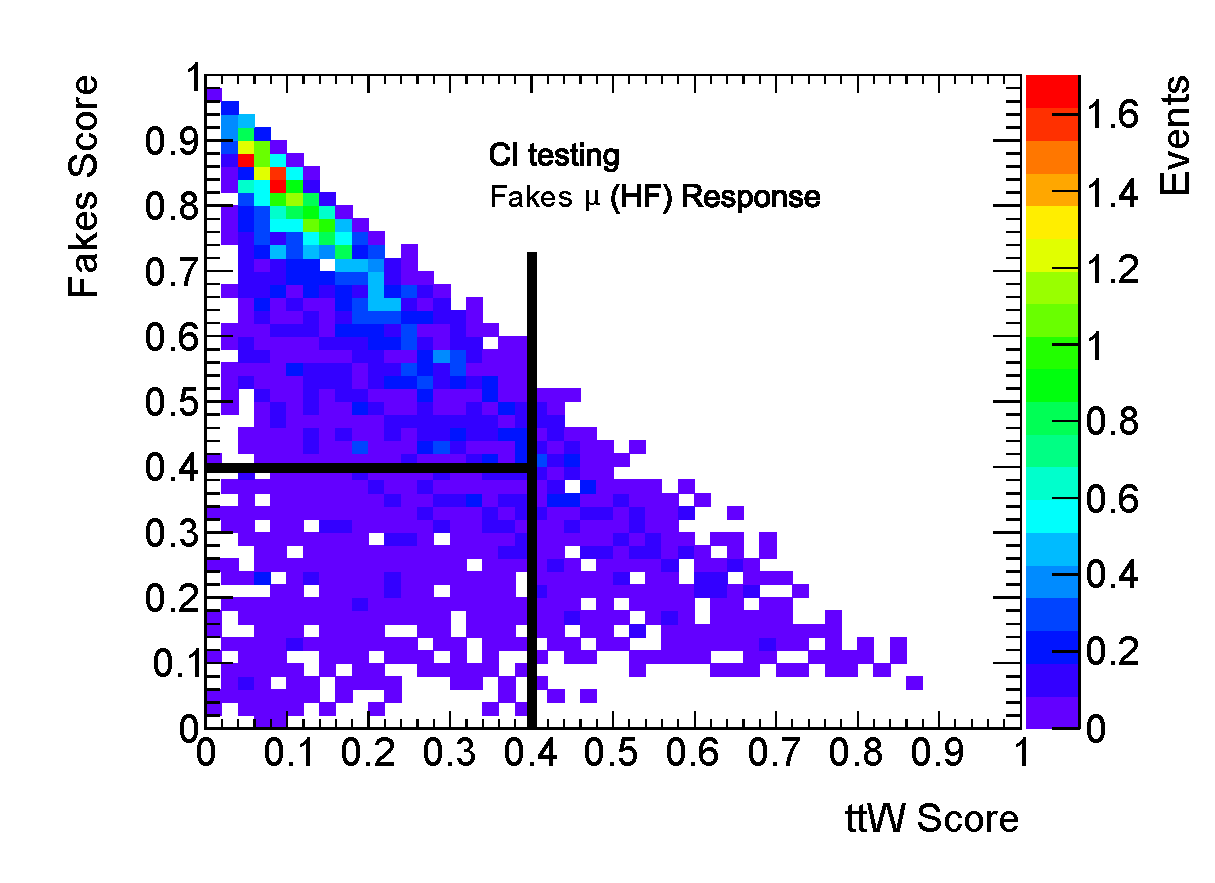
\includegraphics[width=.4\textwidth]{final_config/2d_mva/MyModel_Fakesmu(HF)_2DMVA.eps}
	\caption{2D projection plots of four selected samples showing the distribution of events in respect to the defined class scores. All events lie on a three dimensional plane, thus, the \ttbarZ score is perpendicular to both the \ttbarW and fakes score. The black lines represent the chosen cuts which are based on these plots.}
	\label{fig:Final2DSeparationPlots}
\end{figure}

\begin{table}
	\centering
	\caption{The yields for the cut and count based (left) and the neural network based (right) region definition.}
	\vspace{1mm}
	\resizebox{\textwidth}{!}{%
		\begin{tabular}{lVrrrVrrr}
			& SR-ttZ-CC & CR-ttW-CC & CR-Fakes-CC 	& SR-ttZ-NN & CR-ttW-NN & CR-Fakes-NN\\
			\hline
			$t\bar{t}Z$			& $121\pm4$	& $25\pm2$ 	& $31\pm1$		& $95\pm19$ & $48\pm10$ & $35\pm7$\\
			$t\bar{t}W$			& $26\pm2$ 	& $28\pm2$ 	& $19\pm1$		& $13\pm6$ 	& $46\pm20$ & $13\pm6$\\
			$t\bar{t}H$			& $46\pm4$ 	& $19\pm2$ 	& $16\pm2$		& $33\pm4$ 	& $26\pm3$ & $22\pm2$\\
			%		$WZb$				& $18\pm10$ & $3\pm2$ 	& $5\pm3$		& $10\pm3$ 	& $7\pm2$ & $10\pm3$\\
			%		$WZc$				& $32\pm12$ & $4\pm2$ 	& $10\pm4$		& $16\pm6$ 	& $9\pm4$ & $20\pm8$\\
			%		$WZl$				& $23\pm9$ 	& $3\pm2$ 	& $6\pm3$		& $10\pm4$ 	& $7\pm3$ & $15\pm6$\\
			$WZ$+jets			& $73\pm19$ & $10\pm3$ 	& $21\pm6$		& $36\pm9$ 	& $23\pm6$ & $45\pm12$\\
			%		$ZZb$				& $7\pm4$ 	& $0\pm1$ 	& $3\pm2$		& $3\pm2$ 	& $1\pm1$ & $6\pm2$\\
			%		$ZZc$				& $7\pm3$ 	& $0\pm1$ 	& $3\pm2$		& $3\pm1$ 	& $1\pm1$ & $6\pm3$\\
			%		$ZZl$				& $7\pm3$ 	& $0\pm1$ 	& $4\pm2$		& $3\pm2$ 	& $1\pm1$ & $7\pm3$\\
			$ZZ$+jets			& $20\pm6$ 	& $1\pm1$ 	& $9\pm3$		& $8\pm3$ 	& $3\pm2$ & $18\pm6$\\
			$tZq$				& $13\pm4$ 	& $3\pm1$ 	& $6\pm2$		& $6\pm2$ 	& $8\pm2$ & $8\pm3$\\
			$tWZ$				& $8\pm2$ 	& $3\pm1$ 	& $3\pm1$		& $6\pm2$ 	& $5\pm2$ & $3\pm1$\\
			Fakes $e$ (HF)		& $30\pm2$ 	& $16\pm1$ 	& $20\pm1$		& $8\pm1$ 	& $8\pm1$ & $51\pm7$\\
			Fakes $e$ (Other)	& $46\pm3$ 	& $25\pm1$ 	& $30\pm3$		& $22\pm3$ 	& $33\pm4$ & $46\pm6$\\
			Fakes $\mu$ (HF)	& $41\pm3$ 	& $23\pm1$ 	& $25\pm1$		& $11\pm2$ 	& $12\pm2$ & $65\pm8$\\
			Fakes (Other)		& $19\pm2$ 	& $8\pm1$ 	& $11\pm2$		& $10\pm2$ 	& $10\pm2$ & $18\pm3$\\
			%
			Others				& $8\pm1$ 	& $8\pm1$ 	& $5\pm1$		& $6\pm1$ 	& $11\pm1$ & $3\pm1$\\
			\hline
			Total				& $450\pm24$ & $168\pm6$ & $193\pm9$ 	& $254\pm14$ & $230\pm14$ & $327\pm17$\\
			\hline
			\ttbarZ/Total		& $0.27\pm0.02$ & $0.15\pm0.02$ & $0.16\pm0.01$ & $0.37\pm0.08$ & $0.21\pm0.05$ & $0.11\pm0.03$\\
			\ttbarW/Total		& $0.06\pm0.01$ & $0.17\pm0.02$ & $0.10\pm0.01$ & $0.05\pm0.03$ & $0.20\pm0.09$ & $0.04\pm0.02$\\
			Fakes/Total			& $0.30\pm0.02$ & $0.43\pm0.02$ & $0.45\pm0.03$ & $0.20\pm0.03$ & $0.27\pm0.03$ & $0.55\pm0.05$\\
		\end{tabular}%
	}
	\label{tab:Yields}
\end{table}


\chapter{Neural Networks and Fitting Algorithm}
\label{ch:neural_networks}
The implementation of a machine learning approach such as a deep neural network is expected to increase the quality of region definition. Unlike classical algorithms, neural networks can be programmed to adapt to a given dataset. This adaptation simulates a learning process and hence provides the possibility to train neural networks for certain tasks. Machine learning approaches are widely used in several modern fields of studies such as image recognition \cite{nn_application01}, identification of biological structures \cite{nn_application02} and user-analysis on social media \cite{nn_application03}.

\section{Deep Neural Networks}
In the mid 20$^\text{th}$ century, Warren S. McCulloch and Walter Pitts formulated the first attempt to simulate an artificial network using logical structures similar to the structure of human neurons in the brain \cite{nn_hist01}. In 1957, a machine called \textsc{Mark 1 Perceptron} based on this idea was built by Frank Rosenblatt \cite{nn_hist02}. The machines' network consists of an input layer using an array of photocells and an output layer for the electrical signal. The connections between those layers were weighted by electric potentiometers and could be tweaked by electric motors to simulate a learning process. The performance of this network was limited, since it was an analogue single-layered network. 

Modern neural networks are algorithms which simulate multi-layered deep neural networks (DNN) with several hidden layers between the input and output layer. Figure~\ref{fig:NeuralNetwork} shows a so-called feedforward neural network with one hidden layer. In a feedforward DNN each node of a layer receives a weighted input from every node of the previous layer and emits an output, which will be used in the next layer \cite{nn_nodecalculation}. The output of the hidden layers are usually not stored and thus invisible.

This idea can be described mathematically using a vector $\vec{v}$ for input and $\vec{u}$ for output. The length of these vectors correspond to the number of nodes in the first and last layer \cite{nn_nodecalculation}. The number of hidden layers and their respective multiplicity of nodes are determined by the neural network architecture. Each node has $n$ inputs $x_i$, corresponding weights $w_i$ and an offset $b$ which are all used to calculate the raw activation
\begin{align}
	z = \sum_i^n w_ix_i + b\,.
\end{align}
The raw activation $z$ is used in a chosen activation function $f$ to produce an output $a$ \cite{nn_nodecalculation}. This process per node is shown in Figure~\ref{fig:NeuralNetwork}. Common choices for the activation function $f(z)$ are \textit{tanh}, \textit{Sigmoid}, \textit{ReLU} and \textit{Softmax} \cite{nn_activationfunction}. 

To train a DNN, the given dataset is usually divided into a training and a validation set. The first set is used in the training process to teach the neural network. Each step, a certain batch of samples are used for training the DNN. After the whole training set is used, an epoch is completed and the performance of the neural network is tested on the statistically independent validation set. The improvement for a given epoch is determined by the loss which needs to be minimised \cite{nn_overfitting}. If the neural network trains for too many epochs on a given training dataset, it begins to overfit. This means, the DNN improves its performance on the training set, but worsens on validations sets \cite{nn_overfitting}. Overfitting can be prevented by including some regularisation technique such as early stopping. 

\begin{figure}[t]
	\centering
	\begin{tabular}{m{.5\textwidth} m{.45\textwidth}}
			\includegraphics[width=.52\textwidth]{figures/neural_networks/nn_map.png} &
			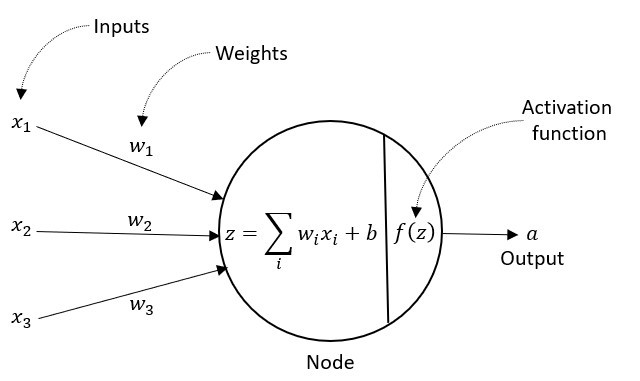
\includegraphics[width=.47\textwidth]{figures/neural_networks/nn_node.png}
	\end{tabular}
	\caption{A schematic visualisation of a feedforward DNN (left) using one hidden layer. Each node can be represented (right) with multiple weighted inputs and an activation function $f$.}  
	\label{fig:NeuralNetwork}
\end{figure}


\section{Neural Network Architecture}
\label{sec:NeuralNetworkArchitecture}
For the analysis, a multi-class approach is used. As mentioned before, the task of the DNN will be to define three class scores that are sensitive to the \ttbarZ, \ttbarW and fakes respectively. The fakes score includes all fake samples with no further subdivision. These scores are used for region definition as described in Section~\ref{sec:NeuralNetworkBasedRegionDefinition}.

The framework used for the neural network is based on \textsc{Keras} \cite{nn_keras}, \textsc{Tensorflow} \cite{nn_tensorflow} and \textsc{scikit-learn} \cite{nn_scikit-learn}. To adjust the neural network, several DNN parameters were individually varied and optimised.

The number of hidden layers and their respective multiplicity of nodes can be chosen to provide enough degrees of freedom to the network \cite{nn_parameters}. For this analysis, 4 layers with 20, 25, 20 and 20 nodes, respectively, were chosen. Additionally, the activation function for the nodes of each layer \cite{nn_activationfunction} must be chosen depending on the desired output. The hidden layers use the \textit{ReLU} activation and the output layer uses \textit{Softmax} activation since it normalises the class scores and thus allows for an easier cut placement. In order to achieve a learning process, the neural network must be trained for a given number of epochs \cite{nn_parameters}. Each epoch, the neural network trains on the training set using the results from previous epochs. The maximum number of epochs is set to 300, however, this value is not reached, since early stopping is implemented and occurs at around 150 epochs. For training, the optimiser \textsc{Nadam} \cite{nn_nadamoptimiser} is implemented. 

The relative size of the validation set must be selected sufficiently large to be representative, however, a smaller validation set allows for a bigger training set. Thus a compromise between those two is chosen carefully and is set to $20\%$. To better utilise the given dataset, $k$-fold cross validation \cite{nn_kfolding} is implemented with 2 folds. Furthermore, the batch size \cite{nn_parameters} as well as the learning rate \cite{nn_nodecalculation} are optimised in dedicated studies resulting in a batch size of 128 events per batch and a learning rate of $0.0005$.

As input for the DNN, several kinematic variables were tested. The chosen variables are expected to be sensitive to either of the three processes and thus the choice is motivated by the underlying physics processes. The DNN uses jet and $b$-jet multiplicity, the missing energy \ETMiss, $\Delta R$ of the OSSF-pair and the three highest \pT of jets and leptons as input. 

The choice to implement jet multiplicity is motivated by the expected signals as explained in Section~\ref{sec:theory_ttZ_ttW} and the reasons for choosing \ETMiss and \dR are discussed in Section~\ref{sec:CountAndCountBasedRegionDefinition}. Including the transverse momentum \pT for both jets and leptons is motivated by the fakes background, which is expected to be sensitive to the low regions of the third lepton's $p_{\text{T}}$ in particular. The additional \pT variables were tested and found to improve the DNN performance. 

Moreover, implementing the sum of lepton charges is also expected to improve the DNN performance, because, as explained in Section~\ref{sec:theory_ttZ_ttW}, the \ttbarW processes happen as initial state radiation. Thus, an asymmetry in the sum of lepton charges is expected for the \ttbarW events but not for \ttbarZ or fakes processes. However, this variable is not included in the analysis, since the used DNN-framework does not support sums of variables as input. Further inputs were tested and found to be non-beneficial for the DNN performance.

The impact of the input variable is analysed for each region and the results are summarised in Figure~\ref{fig:PermutationImportance}. As expected, \dR has the most significant impact for the \ttbarZ score. Similarly, for the fake classification, the third lepton's $p_{\text{T}}$ is found to have the highest impact. Both of these variables also provide approximately equally high separation performance for the \ttbarW classifier. The missing energy has a lower impact than expected. Nevertheless, the \ETMiss impact is highest for the \ttbarW classifier.

\begin{figure}
	\centering
	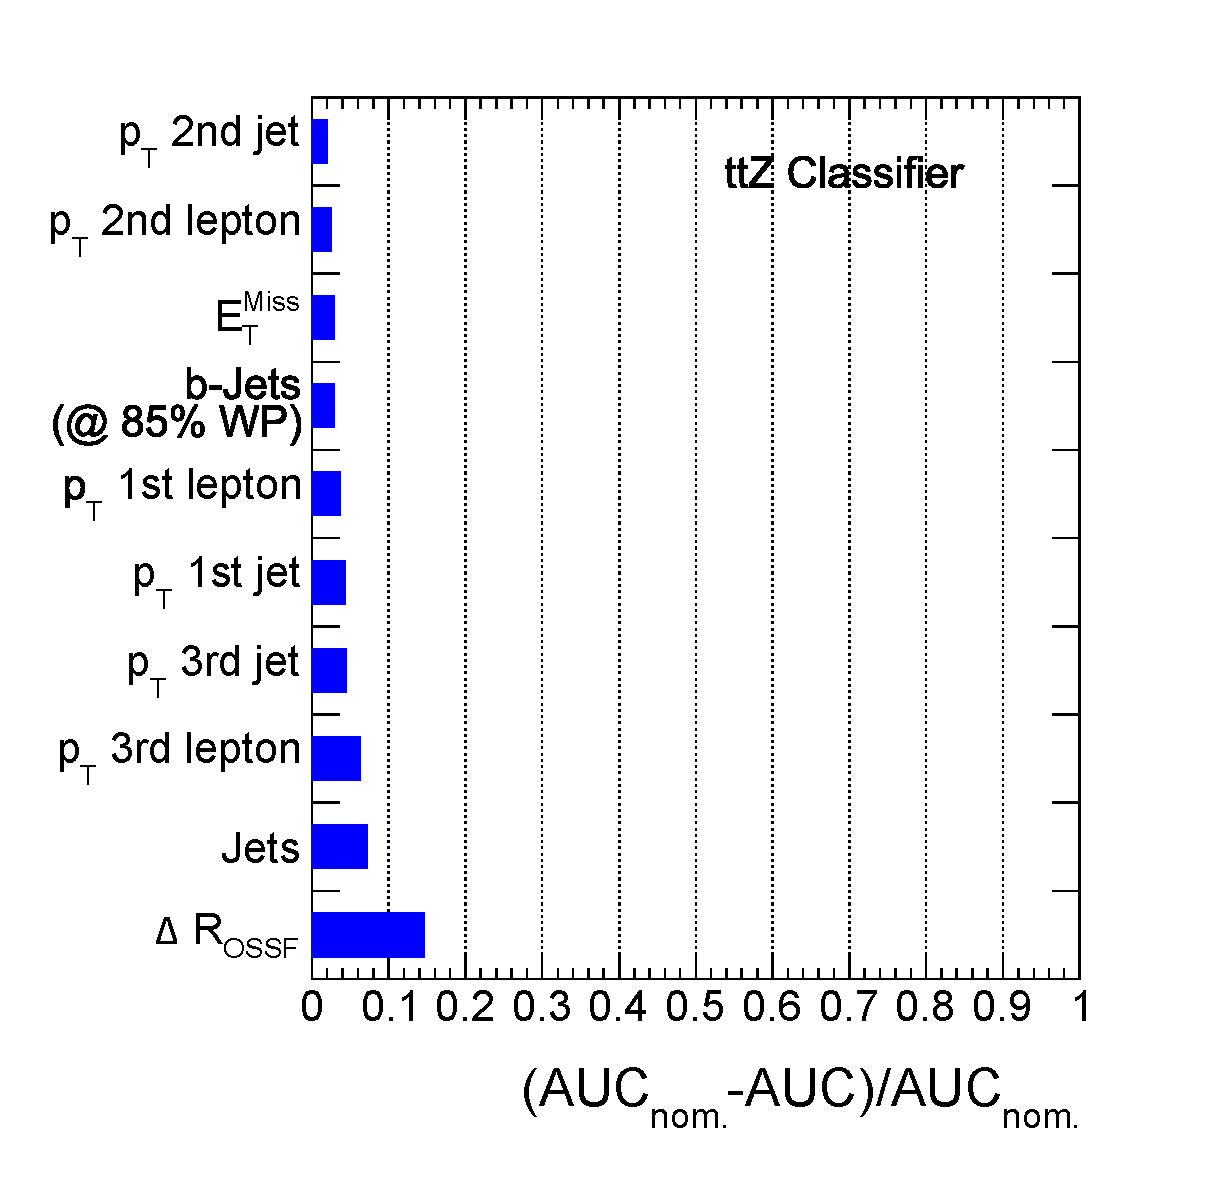
\includegraphics[width=.32\textwidth]{figures/neural_networks/output/MyModel_Permutation_ImportancettZ.eps}
	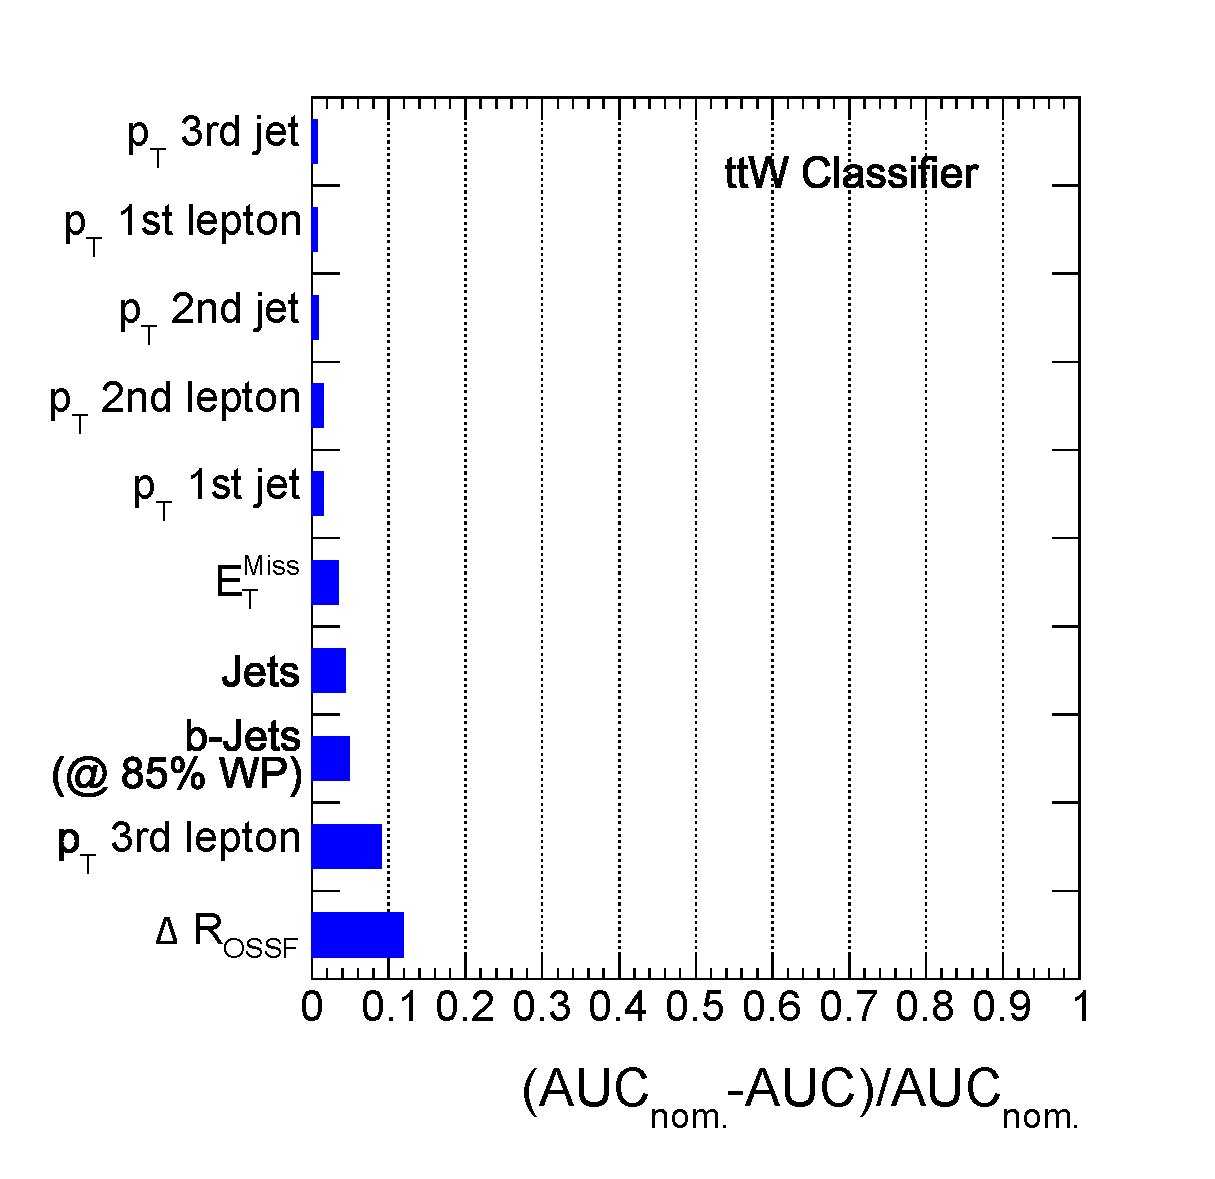
\includegraphics[width=.32\textwidth]{figures/neural_networks/output/MyModel_Permutation_ImportancettW.eps}
	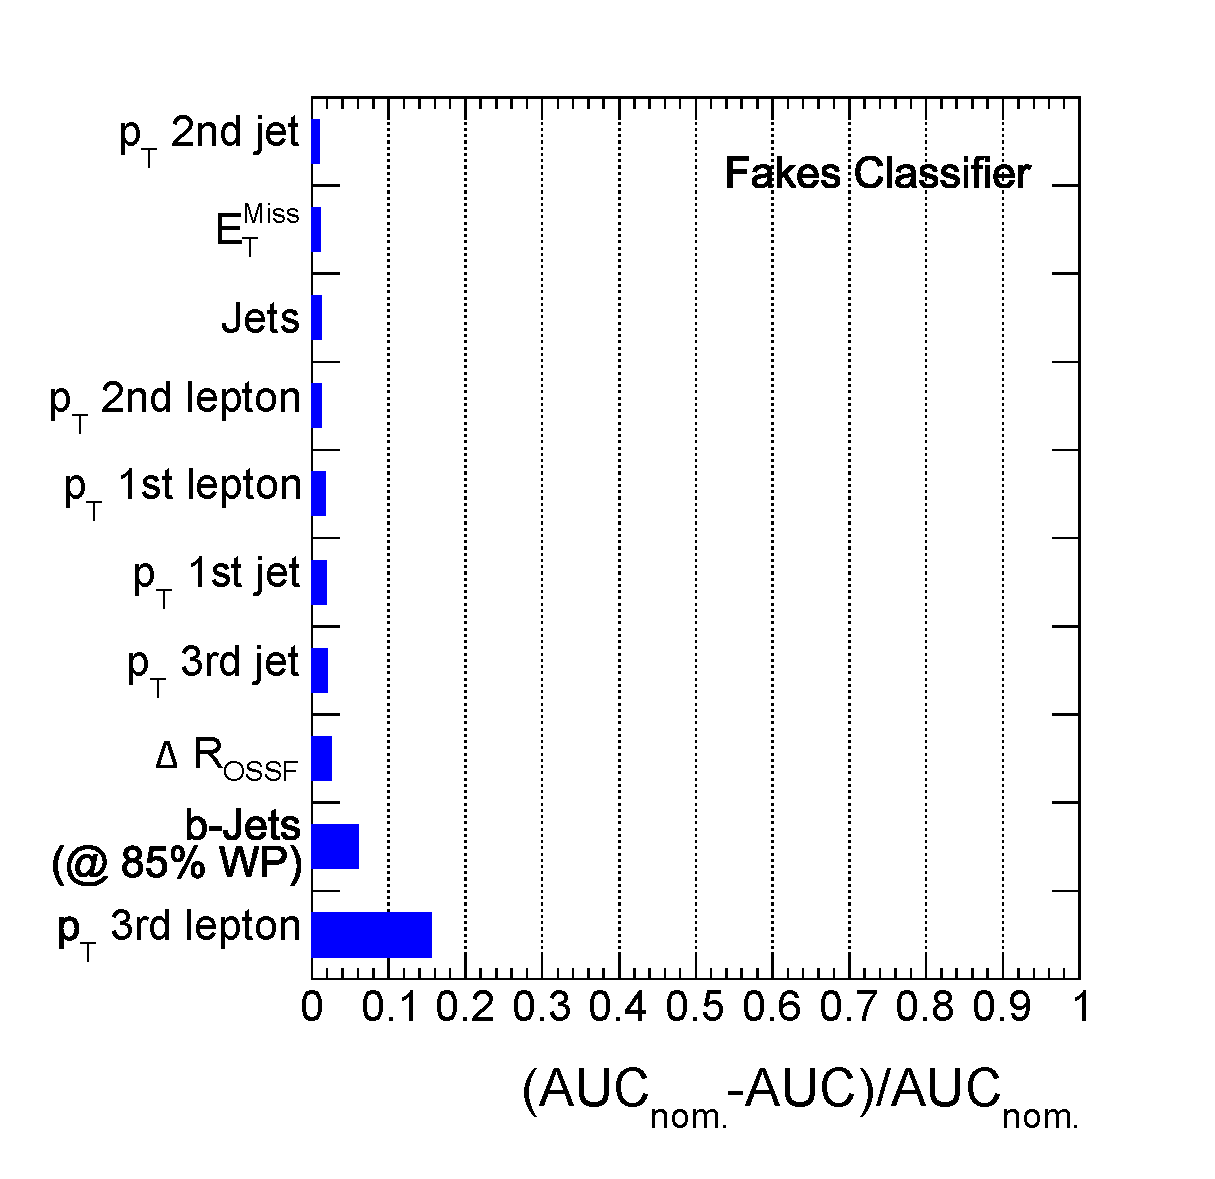
\includegraphics[width=.32\textwidth]{figures/neural_networks/output/MyModel_Permutation_ImportanceFakes.eps}
	\caption{Histograms showing the impact of input variables for the \ttbarZ (left), \ttbarW (centre) and fakes (right) class. The variables are sorted by their impact for each classifier.}
\label{fig:PermutationImportance}
\end{figure}

 To further evaluate the performance of the DNN, confusion matrices for each of the three classifiers are plotted as shown in Figure~\ref{fig:ConfusionMatricies}. Each confusion matrix shows the classification of events per sample. The \ttbarZ classifier shows that high fractions of around $70\%$ of \ttbarZ events have a \ttbarZ score of less than $0.5$. Additionally, these plots show that the separation performance between \ttbarW and the \textit{Others} sample is relatively low. This is expected, since one of the processes included in the \textit{Others} sample is \ttWW which has a similar event signature. Since the \textit{Others} sample has low yields in comparison to \ttbarW, as seen in Table~\ref{tab:Yields}, this will not have a significant impact on the DNN performance. The fake classifier works best on the heavy flavour (HF) fake samples. For the other two fake samples around $\sim60\%$ of events score lower than $0.5$ for the fake classifier. Also, the $WZ$/$ZZ$+jets events achieved relatively high fake class scores. These results are supported by the observed yields for the neural network based configuration in Table~\ref{tab:Yields}.
 
 The overall performance for the defined DNN can be assessed using ROC curves \cite{nn_roccurve}. The area under the curve (AUC) is calculated for each of the folds and is a measure of the DNN performance. The computed integral can be in the range of $[0,1]$, values close to 0.5 indicate a bad performance that is comparable to guessing. Very performant DNN would achieve values close to one or zero \cite{nn_roccurve}. The calculated ROC curves are summarised in Figure~\ref{fig:nn_OutputROCCurves} and show, that the \ttbarW classifier achieves the best performance. %Furthermore, for a more detailed analysis all events are classified by the DNN and their distributions are summarised in Figure~\ref{fig:nn_OutputClassification}.
 
\begin{figure}
	\centering
	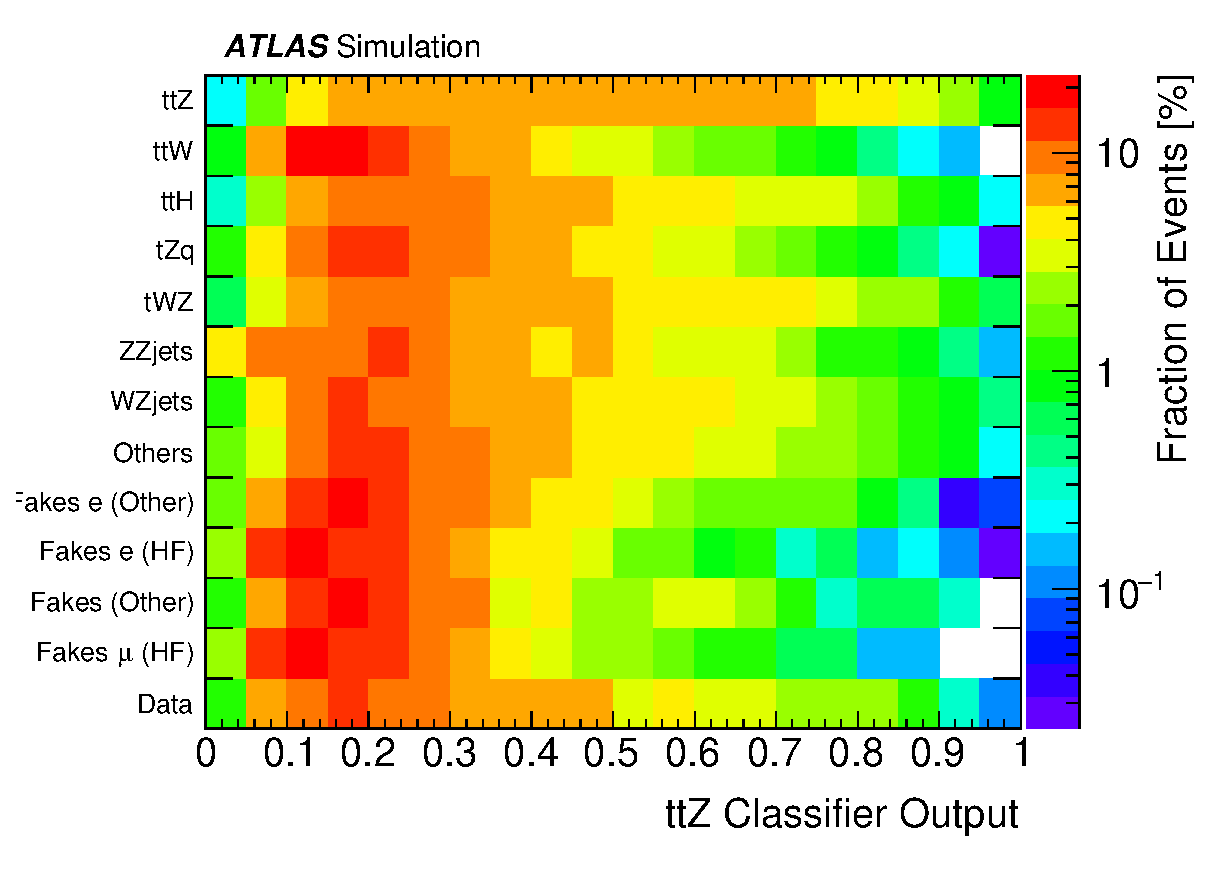
\includegraphics[width=.42\textwidth]{figures/neural_networks/output/MyModel_Confusion_ttZ.eps}
	
	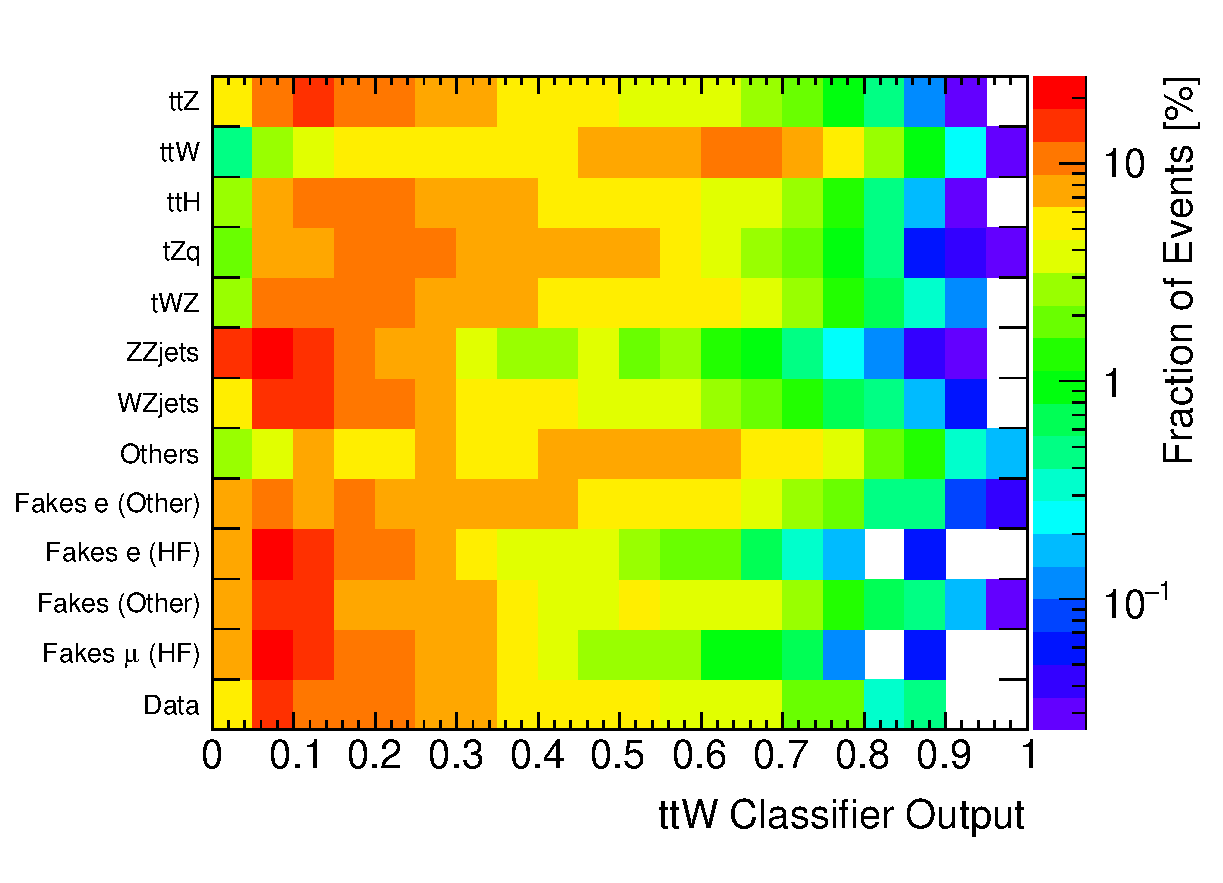
\includegraphics[width=.42\textwidth]{figures/neural_networks/output/MyModel_Confusion_ttW.eps}\hspace{8mm}
	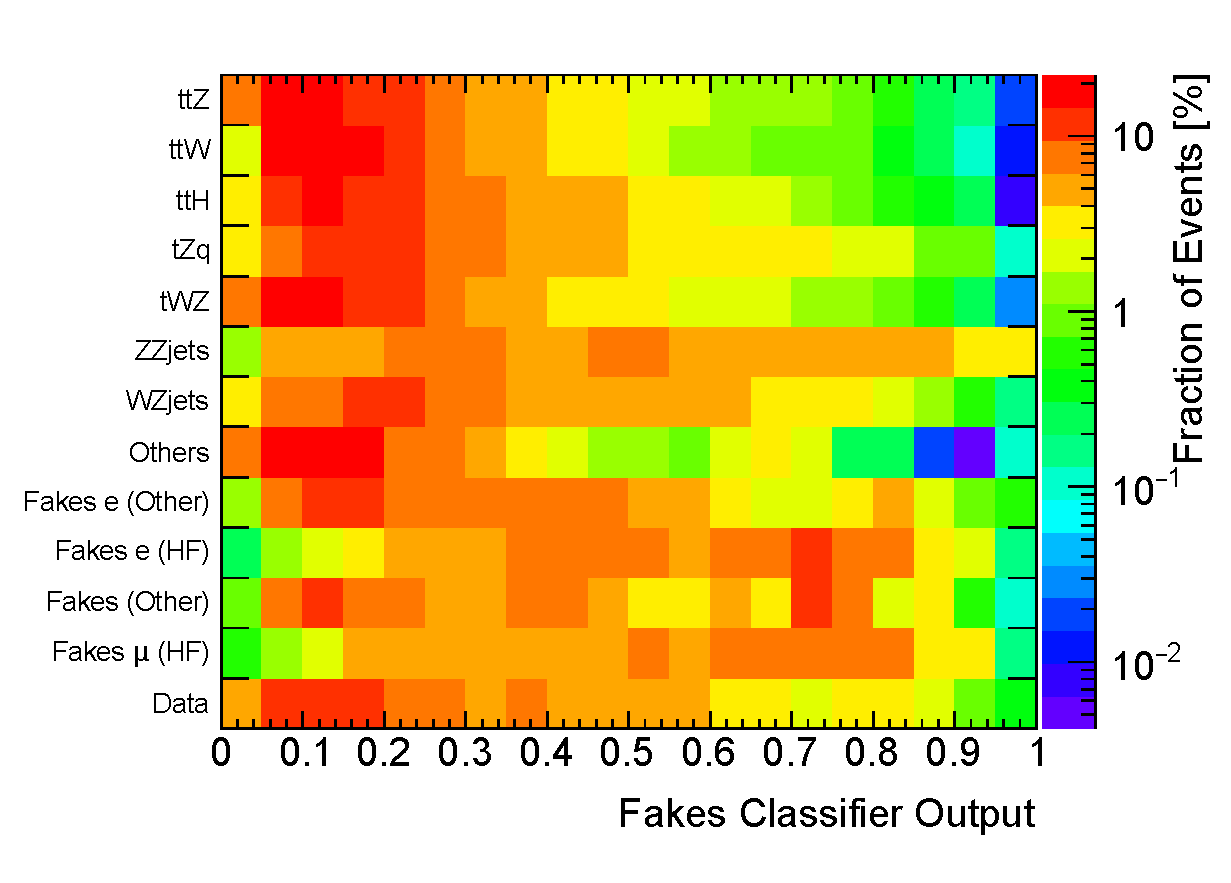
\includegraphics[width=.424\textwidth]{figures/neural_networks/output/MyModel_Confusion_Fakes.eps}
	\caption{The confusion matrices showing the distribution of outputs separated into each sample for the \ttbarZ (top), \ttbarW (bottom left) and fakes (bottom right) classifier.}
	\label{fig:ConfusionMatricies}
\end{figure}

\begin{figure}
	\centering
	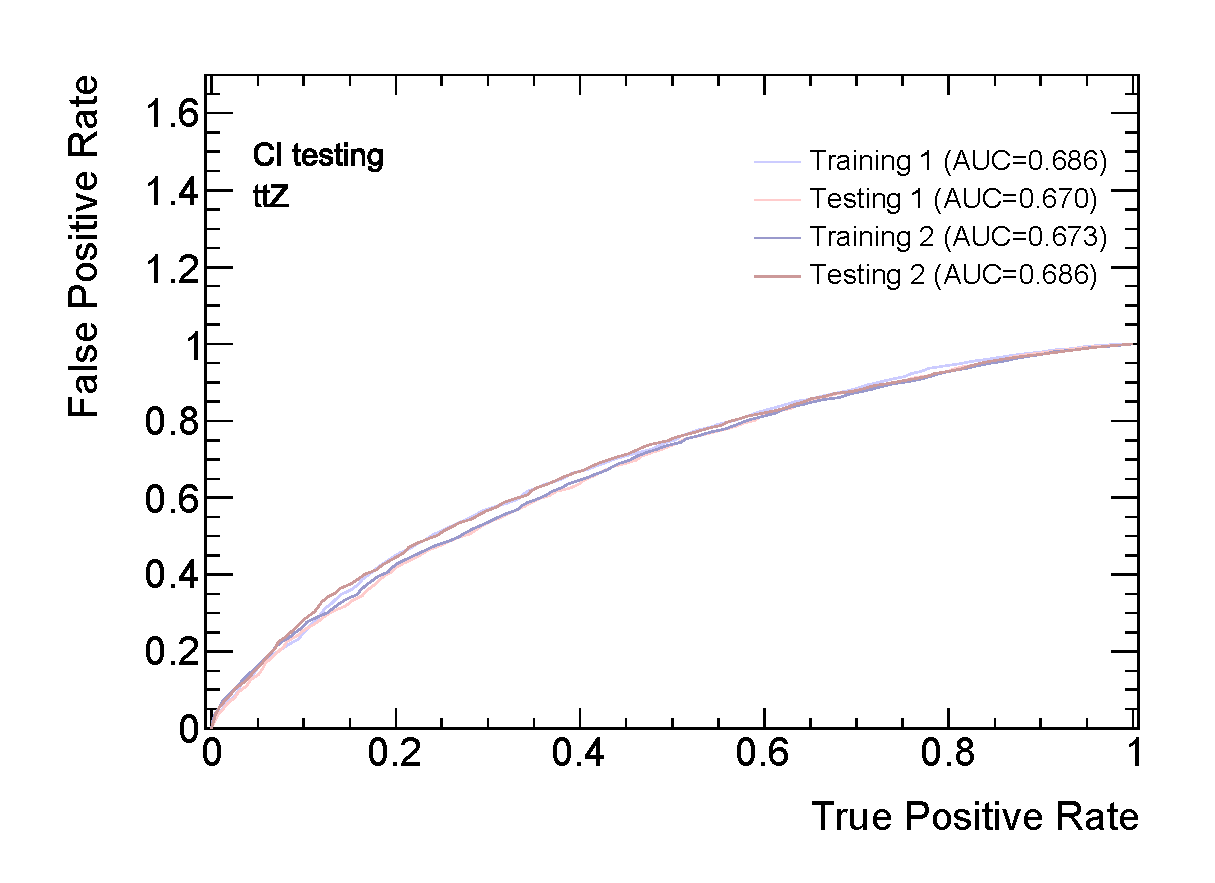
\includegraphics[width=.42\textwidth]{figures/neural_networks/output/MyModel_ROCCurve_Combined_ttZ.eps}
	
	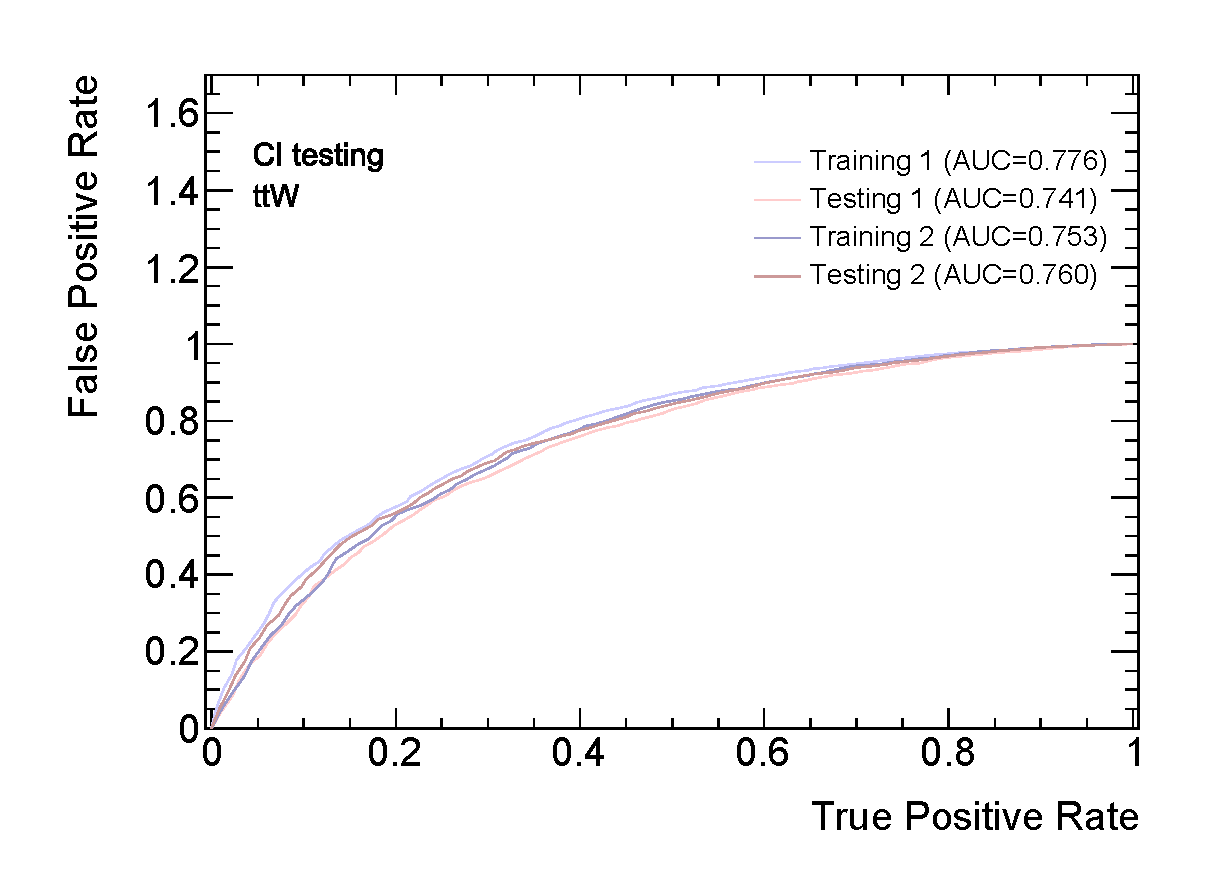
\includegraphics[width=.42\textwidth]{figures/neural_networks/output/MyModel_ROCCurve_Combined_ttW.eps}\hspace{8mm}
	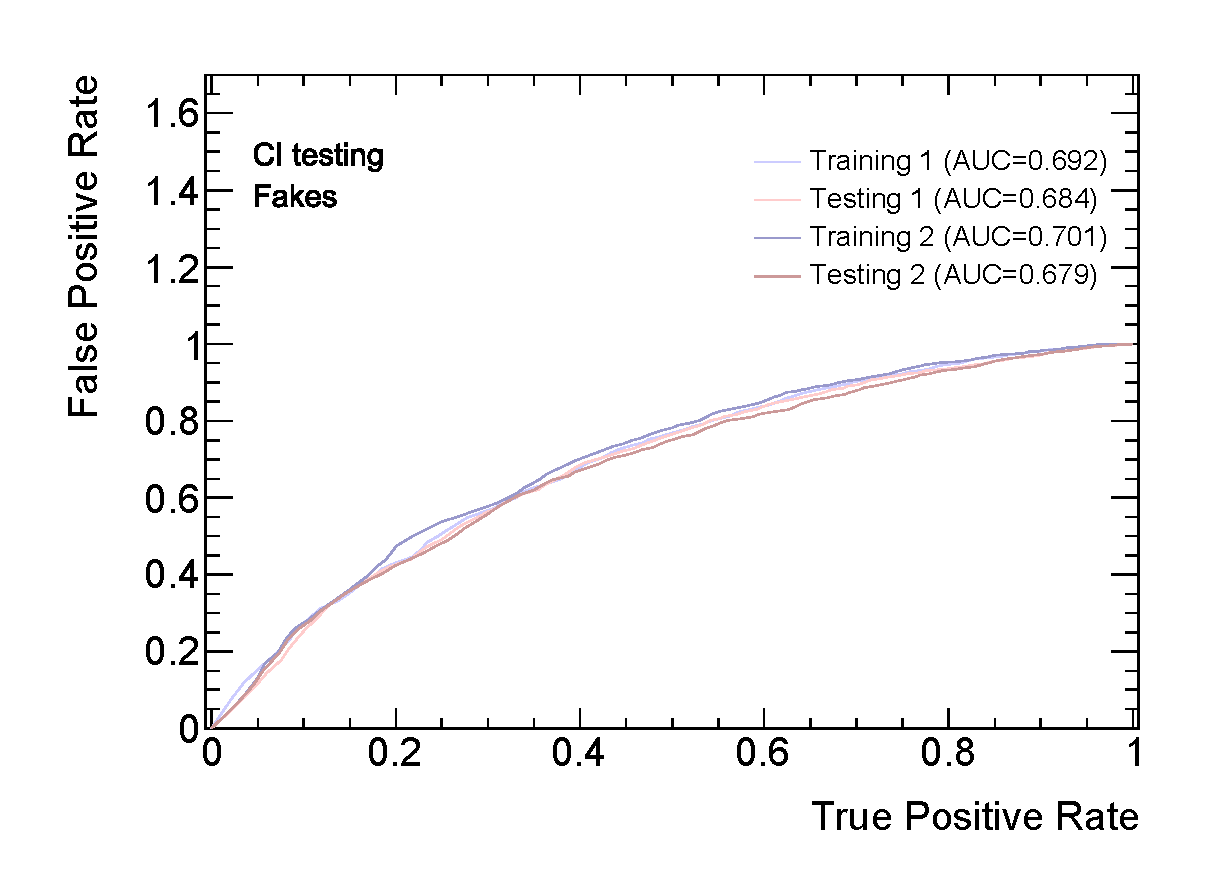
\includegraphics[width=.42\textwidth]{figures/neural_networks/output/MyModel_ROCCurve_Combined_Fakes.eps}
	\caption{The ROC curves showing the performance for the \ttbarZ (top), \ttbarW (bottom left) and fakes (bottom right) class. The training and testing number refers to the $k$-fold.}
	\label{fig:nn_OutputROCCurves}
\end{figure}
%
%\begin{figure}
%	\centering
%	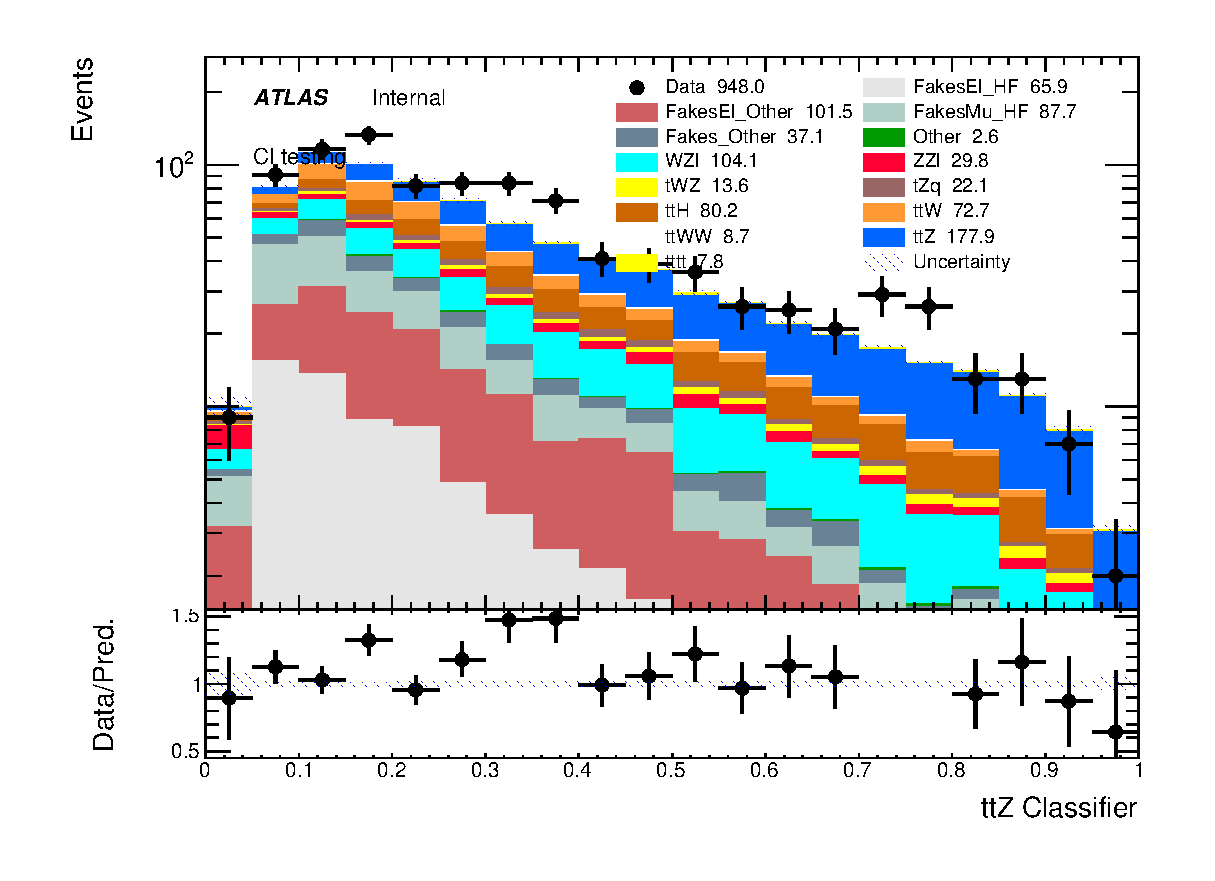
\includegraphics[width=.42\textwidth]{figures/neural_networks/output/MyModel_Classification-DNN_ttZ.eps}
%	
%	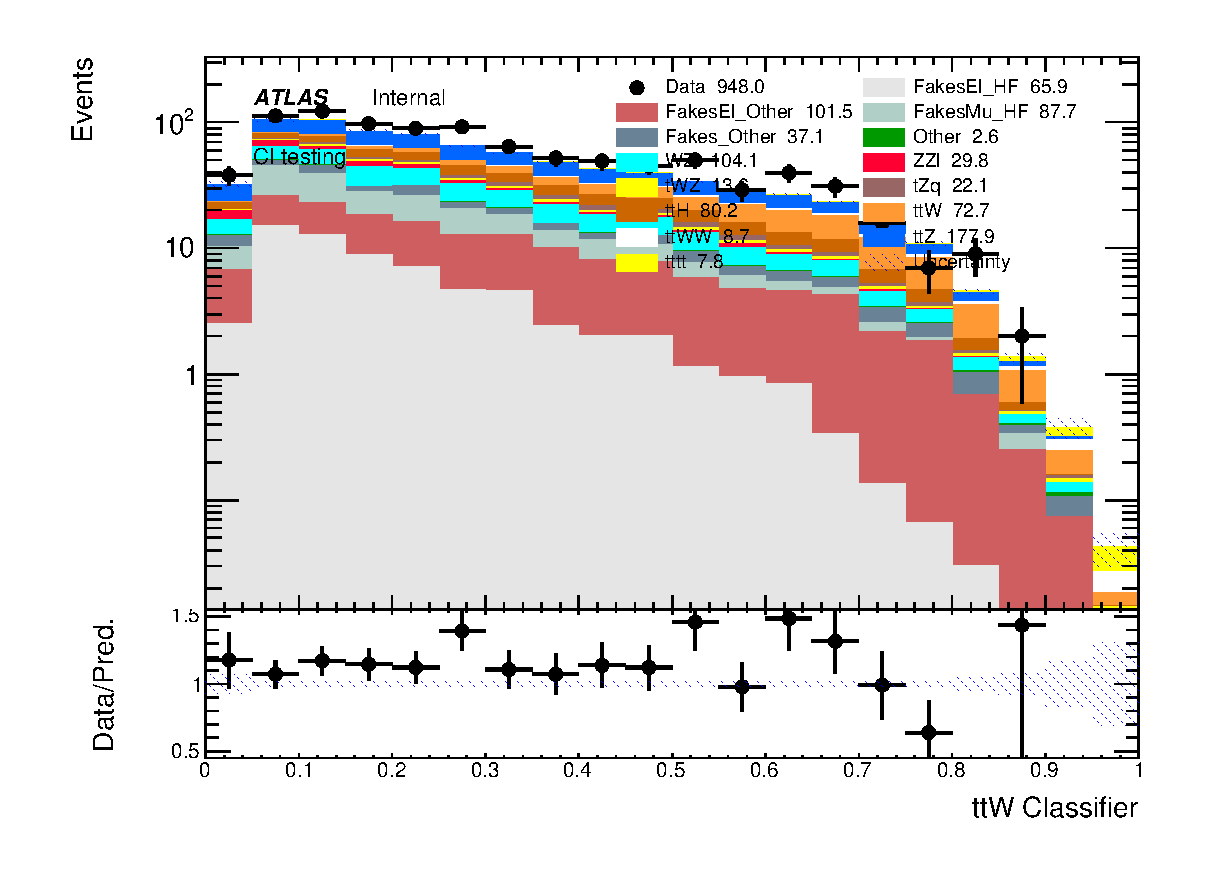
\includegraphics[width=.42\textwidth]{figures/neural_networks/output/MyModel_Classification-DNN_ttW.eps}\hspace{8mm}
%	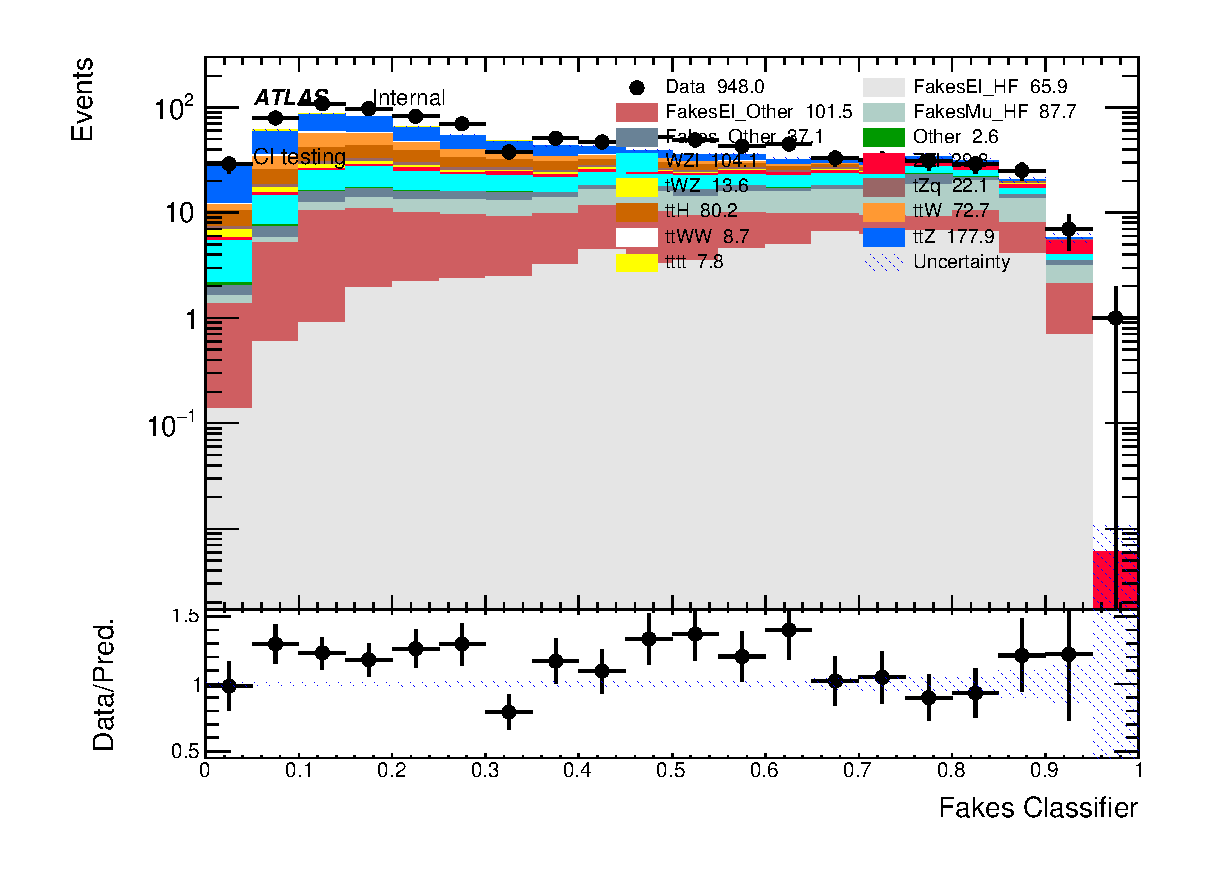
\includegraphics[width=.42\textwidth]{figures/neural_networks/output/MyModel_Classification-DNN_Fakes.eps}
%	\caption{The distribution plots showing the different samples classified by the (top) \ttbarZ, (bottom left) \ttbarW, (bottom right) fakes classifier.}
%	\label{fig:nn_OutputClassification}
%\end{figure}
%\begin{table}
%	\renewcommand{\arraystretch}{1.5}
%	\centering
%	\caption{Values of several parameters for the used DNN.}
%	\begin{tabular}{l|l}
%		Parameter & Value \\
%		\hline
%		Training optimiser				& Nadam \\
%		Hidden layers					& 4\\
%		Node multiplicity 				& (20, 25, 20, 20)\\
%		Hidden activation function		& ReLU\\
%		Output activation function		& Softmax\\
%		Epochs							& 300 (Early stop at $\sim250$)\\
%		Batch size						& 128\\
%		Validation size					& 20\%\\
%		folds							& 2\\
%		Learning rate					& 0.0005\\
%	\end{tabular}
%	\label{tab:NeuralNetworkArchitecture}
%\end{table}

\section{Fitting Algorithm}
\label{sec:FittingAlgorithm}
For the fitting process, a binned profiled likelihood fit \cite{fitting_profilelikelihood01} is performed. In a likelihood fit, a probability density function $L(\mu,\theta)$ that depends on parameters of interest (PoI) $\mu$ and nuisance parameters (NP) $\theta$ is optimised to describe the observed events as the most likely. The profiled likelihood fit reduces the number of dimensions by expressing the nuisance parameters through the PoI. For the fitting process, a dataset in which the model parameters are set to their expected value is generated and used instead of the data set. The value of the PoI used in the fit is set to one. 

Furthermore, for each NP with a Gaussian distribution of mean $\mu$ and width $\sigma$, the pull 
\begin{align*}
	g = \frac{x-\mu}{\sigma}
\end{align*}
can be defined and will be distributed as a standard Gaussian. A deviation of the pulls' mean from zero, is an indicator for possible forms of bias. Uncertainties different to $\pm1$ represent constraints for a given NP \cite{fitting_pullplots}.

This analysis fits the signal strength \muttZ and two normalisation factors \NttW, \NFakes as PoI simultaneously. The included uncertainties described in Chapter~\ref{ch:theoretical_and_experimental_systematic_uncertainties} are implemented as NP. The results of the fitting process are given in Chapter~\ref{ch:measurements_of_the_inclusive_cross_section}.


\chapter{Experimental and Theoretical Systematic Uncertainties}
\label{ch:theoretical_and_experimental_systematic_uncertainties}
The study includes several uncertainties on the used event samples to consider possible deviations from the predicted values. The included uncertainties can be subdivided into experimental uncertainties, which cover the identification and reconstruction of objects inside the detector, and theoretical uncertainties, which cover modelling and estimation variability. In the fitting process, these uncertainties are implemented as nuisance parameters. Up-to-date recommendations of several performance groups are used to determine the uncertainty size. 

\section{Experimental Uncertainties}
\label{sec:UncertaintiesExperimental}
The uncertainty on the luminosity of $139\,\unit{fb}^{-1}$ for the combined \runii dataset is measured to be $1.7\%$ by the official luminosity working group using the LUCID-2 detector \cite{uncertainty_luminosity02} and scans for $x$-$y$ beam-separation by following a method similar to that described in Reference~\cite{uncertainty_luminosity01}. This nuisance parameter is applied to all MC samples.  

Uncertainties related to pile up in the detector \cite{uncertainty_pileup} are implemented to match the data and MC distributions by rescaling the pile-up correction factors during the reweighting. This nuisance parameter is symmetrised using the average of two variations for the upper and lower uncertainty. The total impact of these effects is around 0.2\%-1.0\% per sample.

For the lepton selection, NP for several efficiencies such as trigger, reconstruction, identification and signal isolation as well as momentum scale and resolution are implemented \cite{uncertainty_lepton01, uncertainty_lepton02}. These uncertainties are all symmetrised using two variations and are subdivided into NP for electrons and muons. Each uncertainty individually is below 1\%. Overall there are 51 separate uncertainties for electrons and 37 for muons. 

For the missing energy, two symmetric NP for the resolution and one NP for the scaling are applied \cite{uncertainty_missingenergy}. Also, three more NP are used for the electron-photon identification and isolation \cite{uncertainty_lepton01}. Each of these six uncertainties has an impact less than 1\%.

Analogous to the leptons, jet uncertainties are implemented for the energy scale (JES), energy resolution (JER) and the vertex tagging (JVT) \cite{uncertainty_jet01}. These were derived from test-beam and collision data, as well as MC simulations. In total, 46 uncertainties are applied, each less than 2\%.

Further uncertainties are applied for the flavour tagging uncertainties. These are separated for $b$-tagging \cite{uncertainty_tagging_b}, $c$-tagging \cite{uncertainty_tagging_c} and light quark tagging \cite{uncertainty_tagging_light}. Measurements for those are done using control samples in data and MC to calculate correction factors to correct the rates of flavour tagging in the simulations. In total, 85 uncertainties each less than 2\% are applied for flavour tagging. Each of them is also symmetrised by averaging an up- and down-variation.

\section{Theoretical Uncertainties}
\label{sec:UncertaintiesTheoretical}
For the theoretical prediction of the \ttbarZ events, several uncertainties are implemented. The evaluation of the renormalisation scale $\mu_\text{r}$ and factorisation scale $\mu_\text{f}$ uncertainty is done by varying \textsc{Pythia\,8} samples. This nuisance parameter is not symmetric. Another uncertainty is added for the A14 tune of \textsc{Pythia\,8} \cite{uncertainty_ttZ01} and has an impact of $\sim$2\%. Two additional uncertainties from the choice of PDF are set according to the \textsc{PDF4LHC} recommendation \cite{uncertainty_pdf}, each having an impact less than 0.5\%. The systematic uncertainty for the modelling of the parton shower and the hadronisation is evaluated using alternative samples generated with \textsc{AMC@NLO} \cite{uncertainty_ttZ02} which is interfaced to \textsc{Herwig\,7} \cite{uncertainty_herwig} instead of \textsc{Pythia\,8}. The impact from the shower uncertainty is up to 6.3\% and is symmetrised using one variation.

Most theoretical NP cover the diboson $WZ$+jets and $ZZ$+jets processes. These uncertainties are taken from the most recent \ttbarZ publication \cite{atlas_ttz} in which the uncertainties were determined by comparing data to MC for $Zb$/$Zc$ events and taking heavy flavour jet fraction between $Z$+jets and $ZZ/WZ$+jets into account. Therefore, a flat cross-section uncertainty of $30\%$ is applied to the $ZZc$, $WZc$ and $WZl$ events. For $ZZl$ an uncertainty of $15\%$ is used and for $ZZb$ as well as $WZb$ an uncertainty of $50\%$ is used. Further uncertainties for these processes related to the renormalisation and factorisation scale as well as the PDF choice are derived using the same methods as for the signal \ttbarZ process. Analogously to \ttbarZ, neither nuisance parameters on PDF scale, nor the renormalisation and factorisation are symmetrised.

For the $tWZ$ background, in addition to the diboson NP, an uncertainty for the interference between \ttbarZ and $tWZ$ processes is implemented, which is calculated using the \textsc{DR2} model compared to the \textsc{DR1} model as described in Reference~\cite{uncertainty_tWZ01}. It is evaluated by calculating their modelling difference of uncertainties in the signal regions. This uncertainty is applied symmetrically to the $tWZ$ events. Moreover, a flat normalisation uncertainty of 10\% is applied. 

Following the results of the measurements in Reference~\cite{uncertainty_tZq01}, a flat $14\%$ normalisation uncertainty is applied for the $tZq$ cross-section. PDF and factorisation related uncertainties are again obtained as in the previous samples. Additional uncertainties for the $tZq$ showering and radiation are motivated by the measurements in Reference~\cite{uncertainty_tZq02} and \cite{uncertainty_tZq03}. 

For \ttbarH events, a flat asymmetric uncertainty of $+6.8\%$ and $-9.9\%$ is applied. The implementation of this nuisance parameter covers the uncertainties from QCD scale and PDF choice \cite{uncertainty_ttH01}. 

For additional negligible processes like \tttt or \ttWW a single flat normalisation uncertainty is applied. These minor processes contribute less than $1\%$ to the total yield as seen in \ref{tab:Yields} and thus, a 50\% flat uncertainty is assumed to be sufficient.


\chapter{Measurements of the Inclusive Cross-Section}
\label{ch:measurements_of_the_inclusive_cross_section}
As explained before, to evaluate the simultaneous measurements of \ttbarZ and \ttbarW, the signal strength $\mu_\text{ttZ}$ and two normalisation factors $N_\text{ttW}$ and $N_\text{Fakes}$ for the respective samples are fitted. The normalisation factor $N_\text{Fakes}$ does not separate the four fakes samples but treats them as one group. The fitting process uses a binned profile likelihood fit as described in Section~\ref{sec:FittingAlgorithm} and is done for both region definitions which are summarised in Chapter~\ref{ch:region_definition}.

\section*{Cut and Count Based Configuration}
\label{sec:InitialConfigurationResults}
Figure~\ref{fig:InitialPostFit} shows the post-fit distributions for each region of the cut and count based configuration. As mentioned in Section~\ref{sec:preselection}, the binning is automatically done by an algorithm. The underflow and overflow are included in the first and last bin, respectively. None of the discrepancies between MC data is greater than $3\sigma$. The fitting results for the parameters of interest are 
\begin{align}
	\mu_{t\bar{t}Z} &= 1.00\pm0.22 = 1.00\pm0.19(\text{stat.})\pm0.12(\text{syst.})\\
	N_{t\bar{t}W} 	&= 1.00\pm0.81 = 1.00\pm0.71(\text{stat.})\pm0.39(\text{syst.})\\
	N_\text{Fakes} 	&= 1.00\pm0.20 = 1.00\pm0.18(\text{stat.})\pm0.09(\text{syst.})
\end{align}
whereby the systematic uncertainty is calculated from the statistical and total uncertainty. The ranking plots, which list the most important nuisance parameters, are shown in Figure~\ref{fig:InitialRankingPlots}. Many of the diboson uncertainties are impactful, since the $WZ$/$ZZ$ events have yields comparable to \ttbarW, as seen in Table~\ref{tab:Yields}. Since the analysed channel has low number of events, the luminosity and JET pile up NP are significant for the $\mu_{t\bar{t}Z}$ uncertainty. For the $N_{t\bar{t}W}$ uncertainties, two of the JER related nuisance parameters have an significant impact. The missing energy is crucial for neutrino reconstruction and thus is important for the \ttbarW events, resulting in the significant impact. The ranking for $N_\text{Fakes}$ shows that one of the jet tagging uncertainties has the second highest impact. The correct identification for light jets is important for fakes because these non-prompt leptons have relatively low energies and thus can be misidentified as light jets. All nuisance parameters are also analysed using pull plots in Figure~\ref{fig:PullPlots} and are found to have no significant pull or constrain.

\begin{figure}
	\centering
	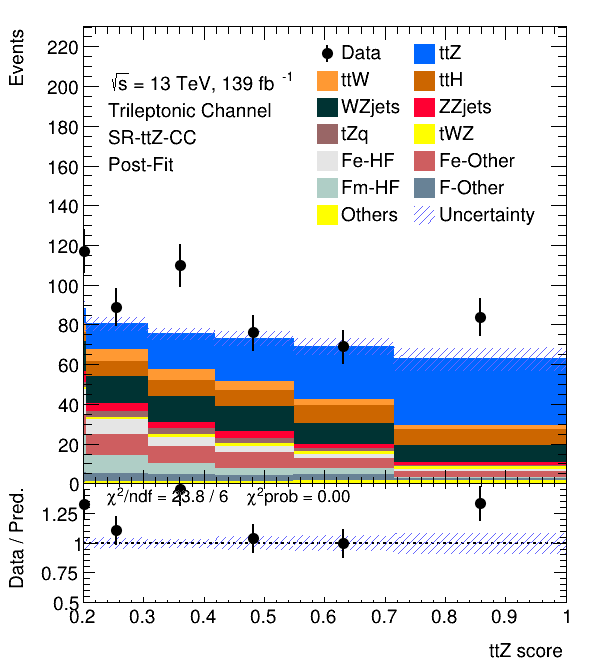
\includegraphics[width=.32\textwidth]{figures/initial_config/distribution/region1_postFit.png}
	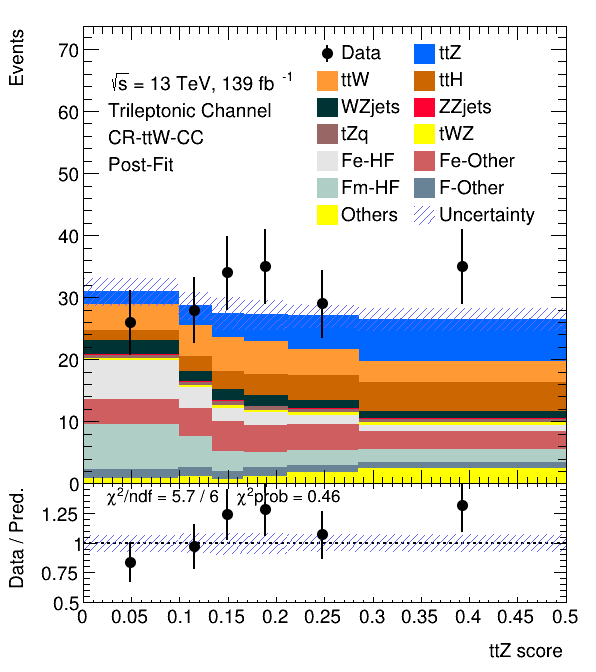
\includegraphics[width=.32\textwidth]{figures/initial_config/distribution/region2_postFit.png}
	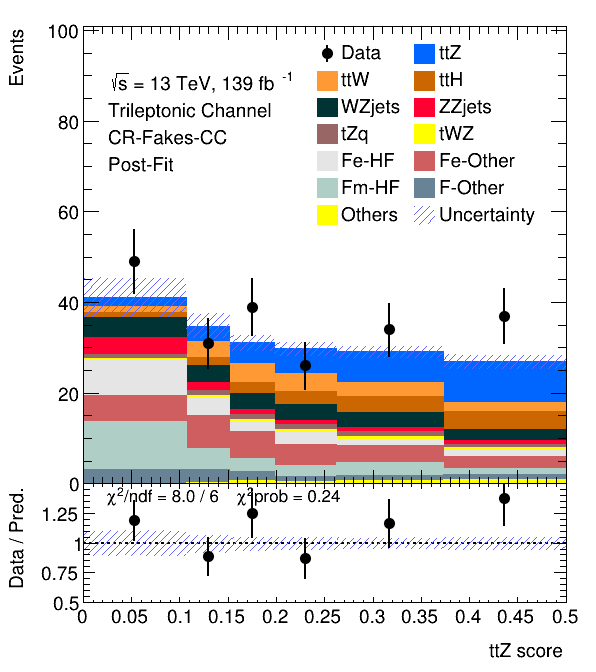
\includegraphics[width=.32\textwidth]{figures/initial_config/distribution/region3_postFit.png}
	
	\caption{The post-fit distributions for the SR-ttZ-CC (left), CR-ttW-CC (centre), CR-Fakes-CC (right) region of the cut and count based configuration.}
	\label{fig:InitialPostFit}
\end{figure}


\begin{figure}
	\centering
	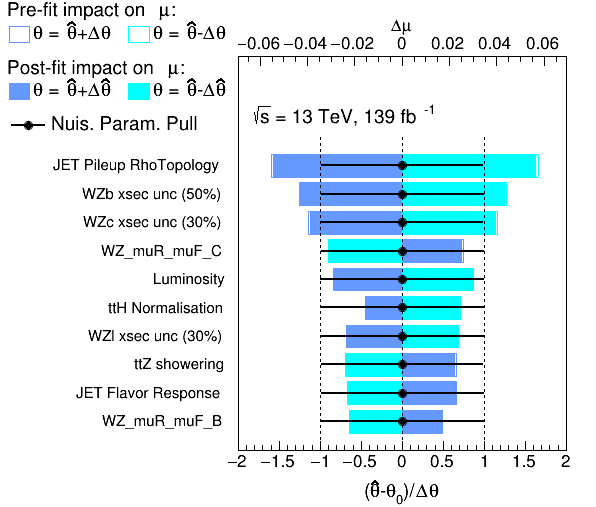
\includegraphics[width=.32\textwidth]{figures/initial_config/ranking/RankingSysts_mu_ttZ_systs.png}
	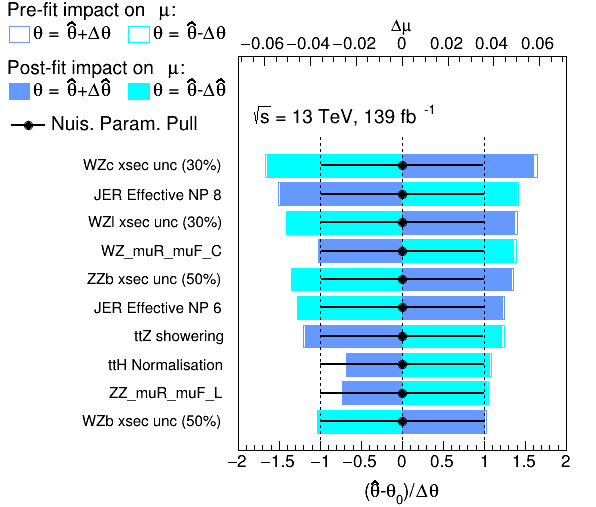
\includegraphics[width=.32\textwidth]{figures/initial_config/ranking/RankingSysts_N_ttW_systs.png}
	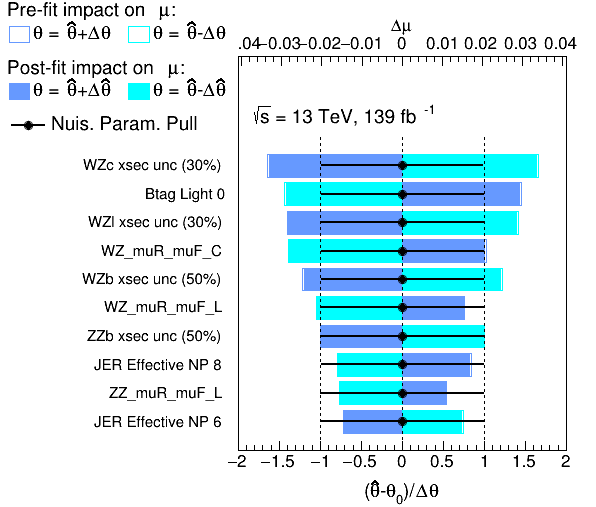
\includegraphics[width=.32\textwidth]{figures/initial_config/ranking/RankingSysts_N_Fakes_systs.png}
	
	\caption{The ranking plots for $\mu_{t\bar{t}Z}$ (left), $N_{t\bar{t}W}$ (centre) and $N_\text{Fakes}$ (right) using the cut and count based regions.}
	\label{fig:InitialRankingPlots}
\end{figure}

%\begin{table}
%	\centering
%	\caption{Fitting results for the uncertainty on the signal strength $\mu_\text{ttZ}$ and the normalisation factors $N_\text{ttW}$ \& $N_\text{Fakes}$ using the cut and count based configuration.}
%	\begin{tabular}{lVlll}
%		& $\sigma_{\mu_\text{ttZ}}$ & $\sigma_{N_\text{ttW}}$ & $\sigma_{N_\text{Fakes}}$\\
%		\hline
%		Stat. 		& $\pm0.19$ & $\pm0.71$ & $\pm0.18$\\
%		Sys.		& $\pm0.12$ & $\pm0.39$ & $\pm0.09$\\
%		\hline
%		Total		& $\pm0.22$ & $\pm0.81$ & $\pm0.20$
%	\end{tabular}
%	\label{tab:InitialResults}
%\end{table}


\section*{Neural Network Based Configuration}
\label{sec:FinalConfigurationResults}
Analogous to the cut and count based configuration, Figure~\ref{fig:FinalPostFitPlots} shows the post-fit distributions for the neural network based configuration. Again, the discrepancies between MC and data are less than $3\sigma$ for all bins. The fitting results are given by 
\begin{align}
	\mu_{t\bar{t}Z} &= 1.00\pm0.24 = 1.00\pm0.18(\text{stat.})\pm0.15(\text{syst.})\\
	N_{t\bar{t}W} 	&= 1.00\pm0.44 = 1.00\pm0.42(\text{stat.})\pm0.14(\text{syst.})\\
	N_\text{Fakes} 	&= 1.00\pm0.14 = 1.00\pm0.12(\text{stat.})\pm0.07(\text{syst.})\,.
\end{align}

The ranking plots in Figure~\ref{fig:FinalRankingPlots} show similar results to the ranking plots from the cut and count based configuration. Most NP are diboson uncertainties for the same reasons as mentioned before. Surprisingly, the jet tagging uncertainty, which is also important for $N_\text{Fakes}$, is the third most impactful NP for $\mu_{t\bar{t}Z}$. This is most likely caused by some neural network classification that is sensitive to this nuisance parameter. These plots also show, that many of the NP, which are impactful on $\mu_{t\bar{t}Z}$, are also impactful on $N_{t\bar{t}W}$. This is expected since these two processes have similar event signatures and are difficult to separate. Moreover, Figure~\ref{fig:PullPlots} shows the pull plots for the neural network based configuration. As before, no significant constrains or pulls are observed.

\begin{figure}
	\centering
	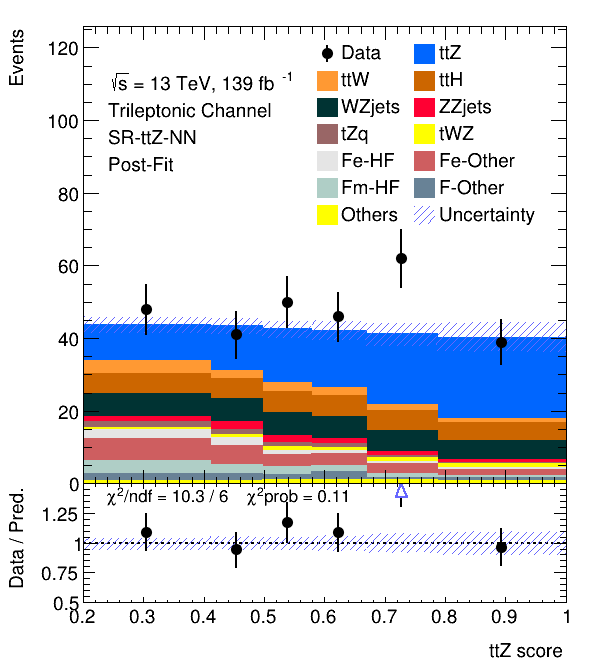
\includegraphics[width=.32\textwidth]{figures/final_config/distribution/SR-offZ-ttZ_postFit.png}
	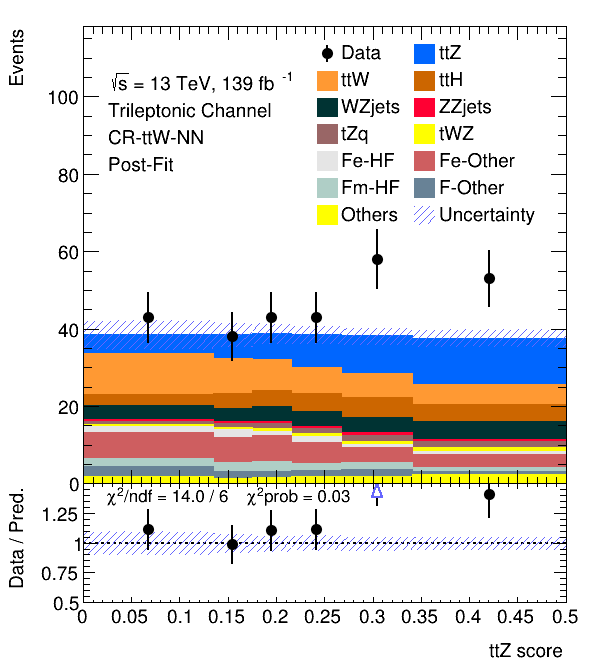
\includegraphics[width=.32\textwidth]{figures/final_config/distribution/CR-offZ-ttW_postFit.png}
	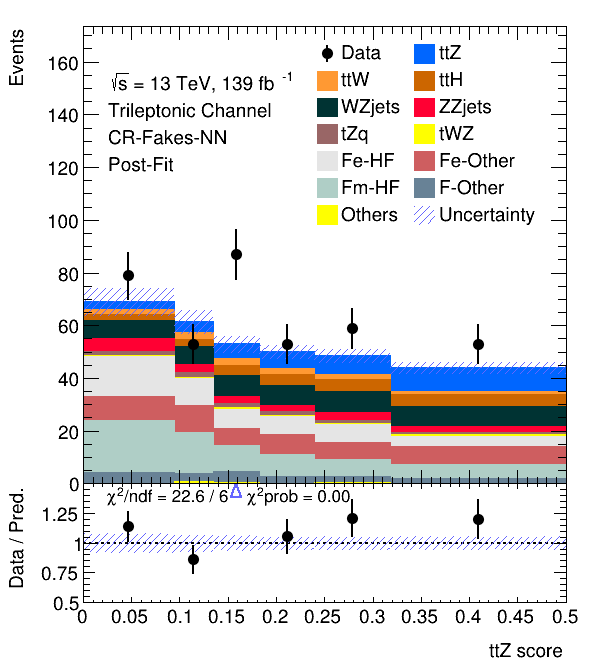
\includegraphics[width=.32\textwidth]{figures/final_config/distribution/CR-offZ-Fakes_postFit.png}
	
	\caption{The post-fit distributions for the SR-ttZ-NN (left), CR-ttW-NN (centre), CR-Fakes-NN (right) region of the neural network based configuration.}
	\label{fig:FinalPostFitPlots}
\end{figure}

\begin{figure}
	\centering
	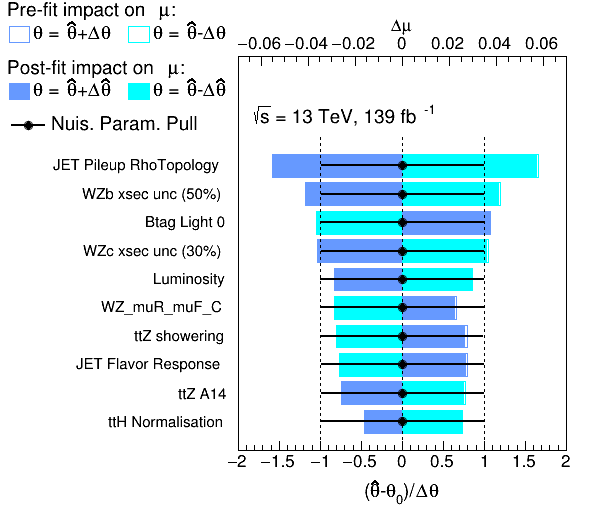
\includegraphics[width=.32\textwidth]{figures/final_config/ranking/RankingSysts_mu_ttZ_systs.png}
	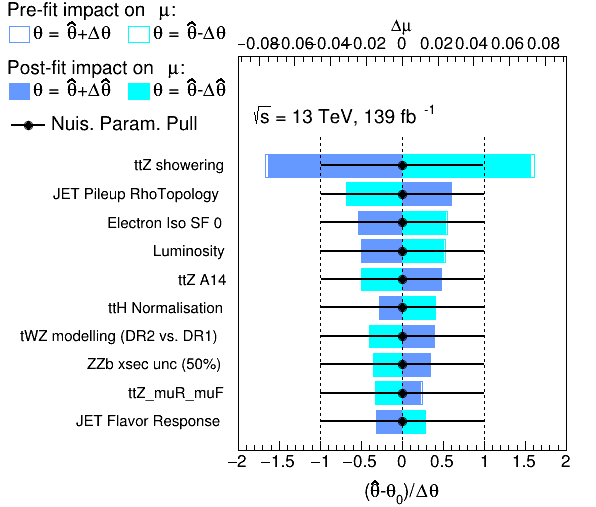
\includegraphics[width=.32\textwidth]{figures/final_config/ranking/RankingSysts_N_ttW_systs.png}
	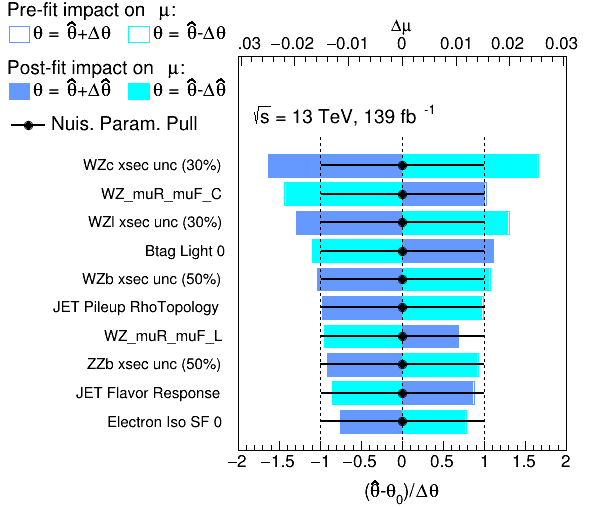
\includegraphics[width=.32\textwidth]{figures/final_config/ranking/RankingSysts_N_Fakes_systs.png}
	
	\caption{The ranking plots for $\mu_{t\bar{t}Z}$ (left), $N_{t\bar{t}W}$ (centre) and $N_\text{Fakes}$ (right) using the neural network based regions.}
	\label{fig:FinalRankingPlots}
\end{figure}

\section*{Comparison}
Comparing the yields for both configurations in Table~\ref{tab:Yields} shows that the neural network based configuration has cleaner regions. The relative number of \ttbarZ events in the signal region has increased by $10\%$, while the relative number of \ttbarW and fake events has decreased by $1\%$ and $10\%$, respectively. Similar results can be observed for the control regions with the exception, that the neural network based \ttbarW control region has $6\%$ more \ttbarZ events compared to the cut and count based one. 

The uncertainty on the PoI for normalisation has decreased by $37\%$ for \ttbarW and $6\%$ for fakes. Both the statistical and systematic uncertainty is halved for $N_{t\bar{t}W}$ using the neural network based configuration. For $N_\text{Fakes}$, the improvements are mostly for statistical uncertainties. The uncertainty of $\mu_{t\bar{t}Z}$, however, is increased by $2\%$. This increase is most likely caused by the low statistics in the neural network based signal region. Comparing the total values in Table~\ref{tab:Yields} shows, that the SR-ttZ-NN has $44\%$ less events compared to SR-ttZ-CC. 

Although the neural network has refined the region definition, the limited statistics for analysed channel restrict the improvements on the signal strength $\mu_{t\bar{t}Z}$ in the fitting processes. Hence, if only the signal strength $\mu_{t\bar{t}Z}$ is analysed, the cut and count based configuration should be used. However, for a simultaneous analysis, it is recommended to use the neural network based configuration because of its overall performance.

To reduce the uncertainties due to low statistics, more events need to be measured. The High-Luminosity \lhc upgrade after \runiii is planned to provide an integrated luminosity of $250\,\unit{fb}^{-1}$ per year \cite{highlumiupgrade}. This could also improve the DNN training since a greater dataset for training can be used.

\begin{figure}
	\centering
	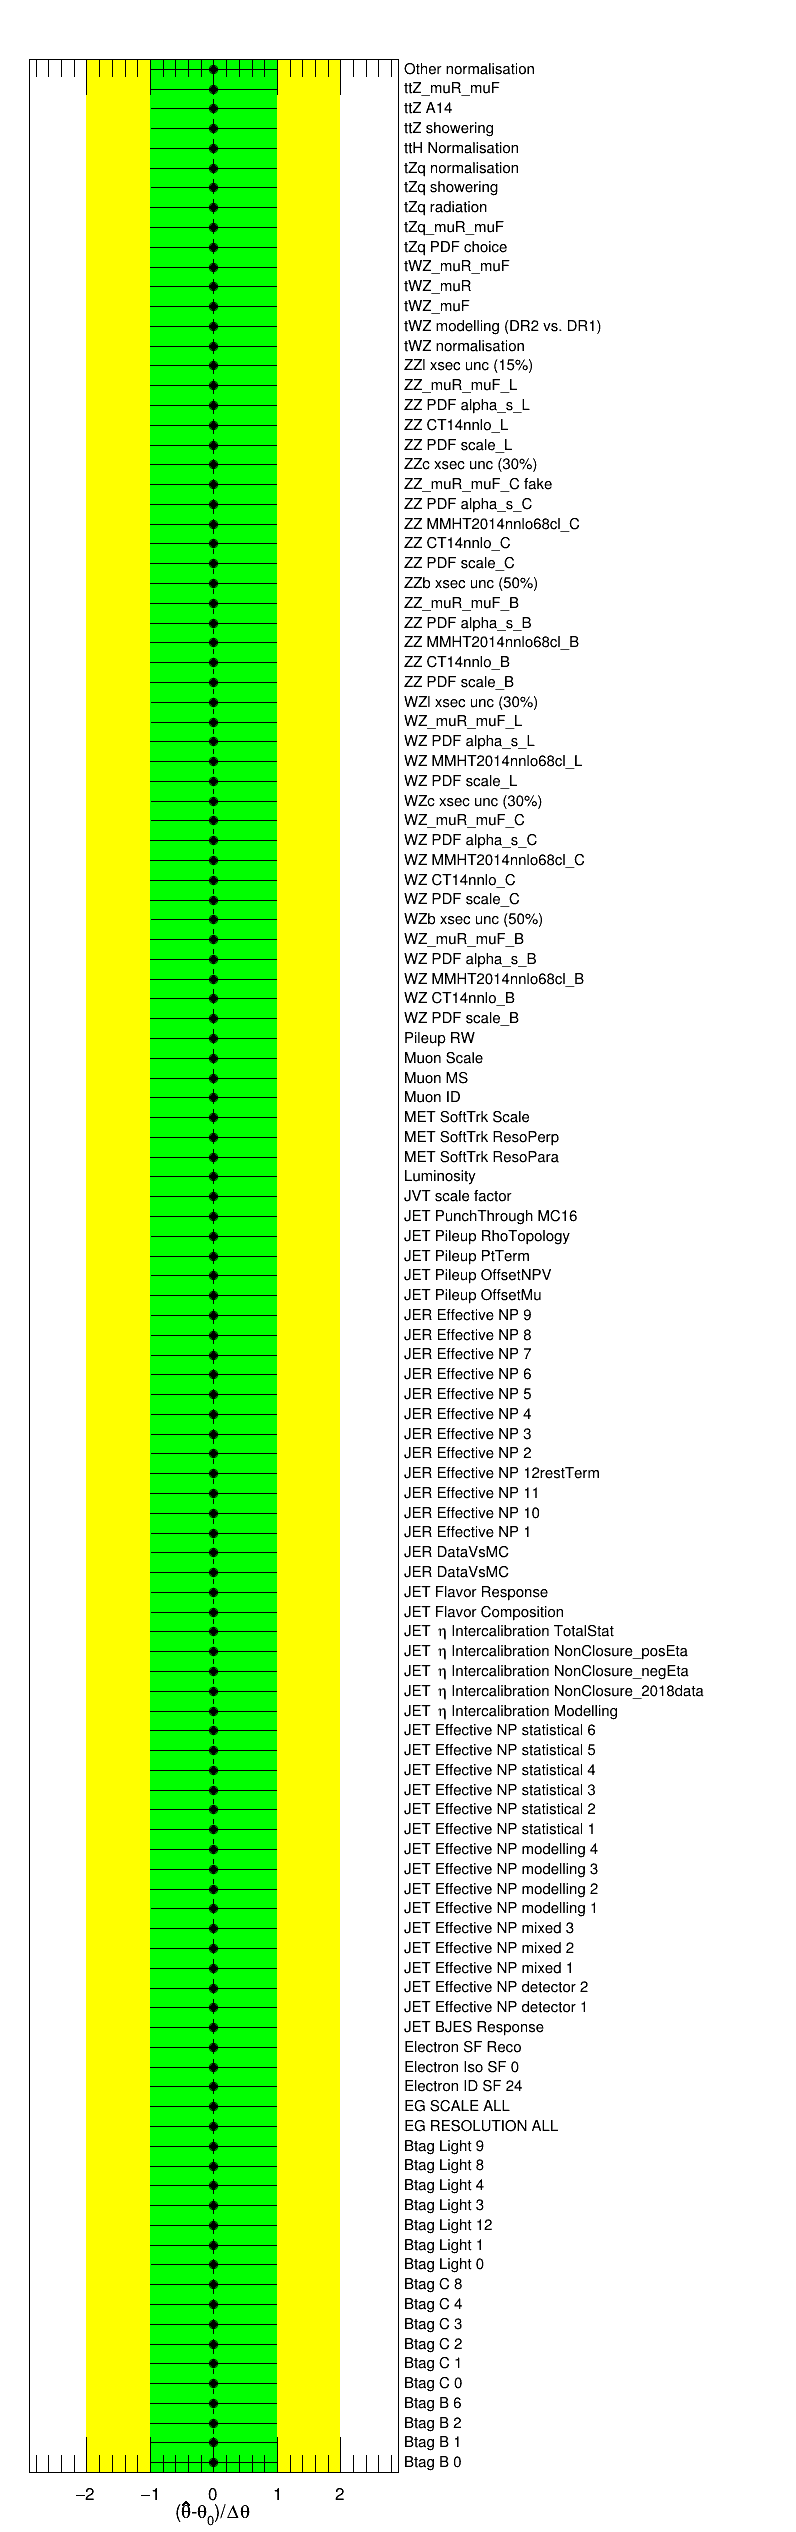
\includegraphics[width=.44\textwidth]{figures/initial_config/pullplots/NuisPar.png}\hspace{8mm}
	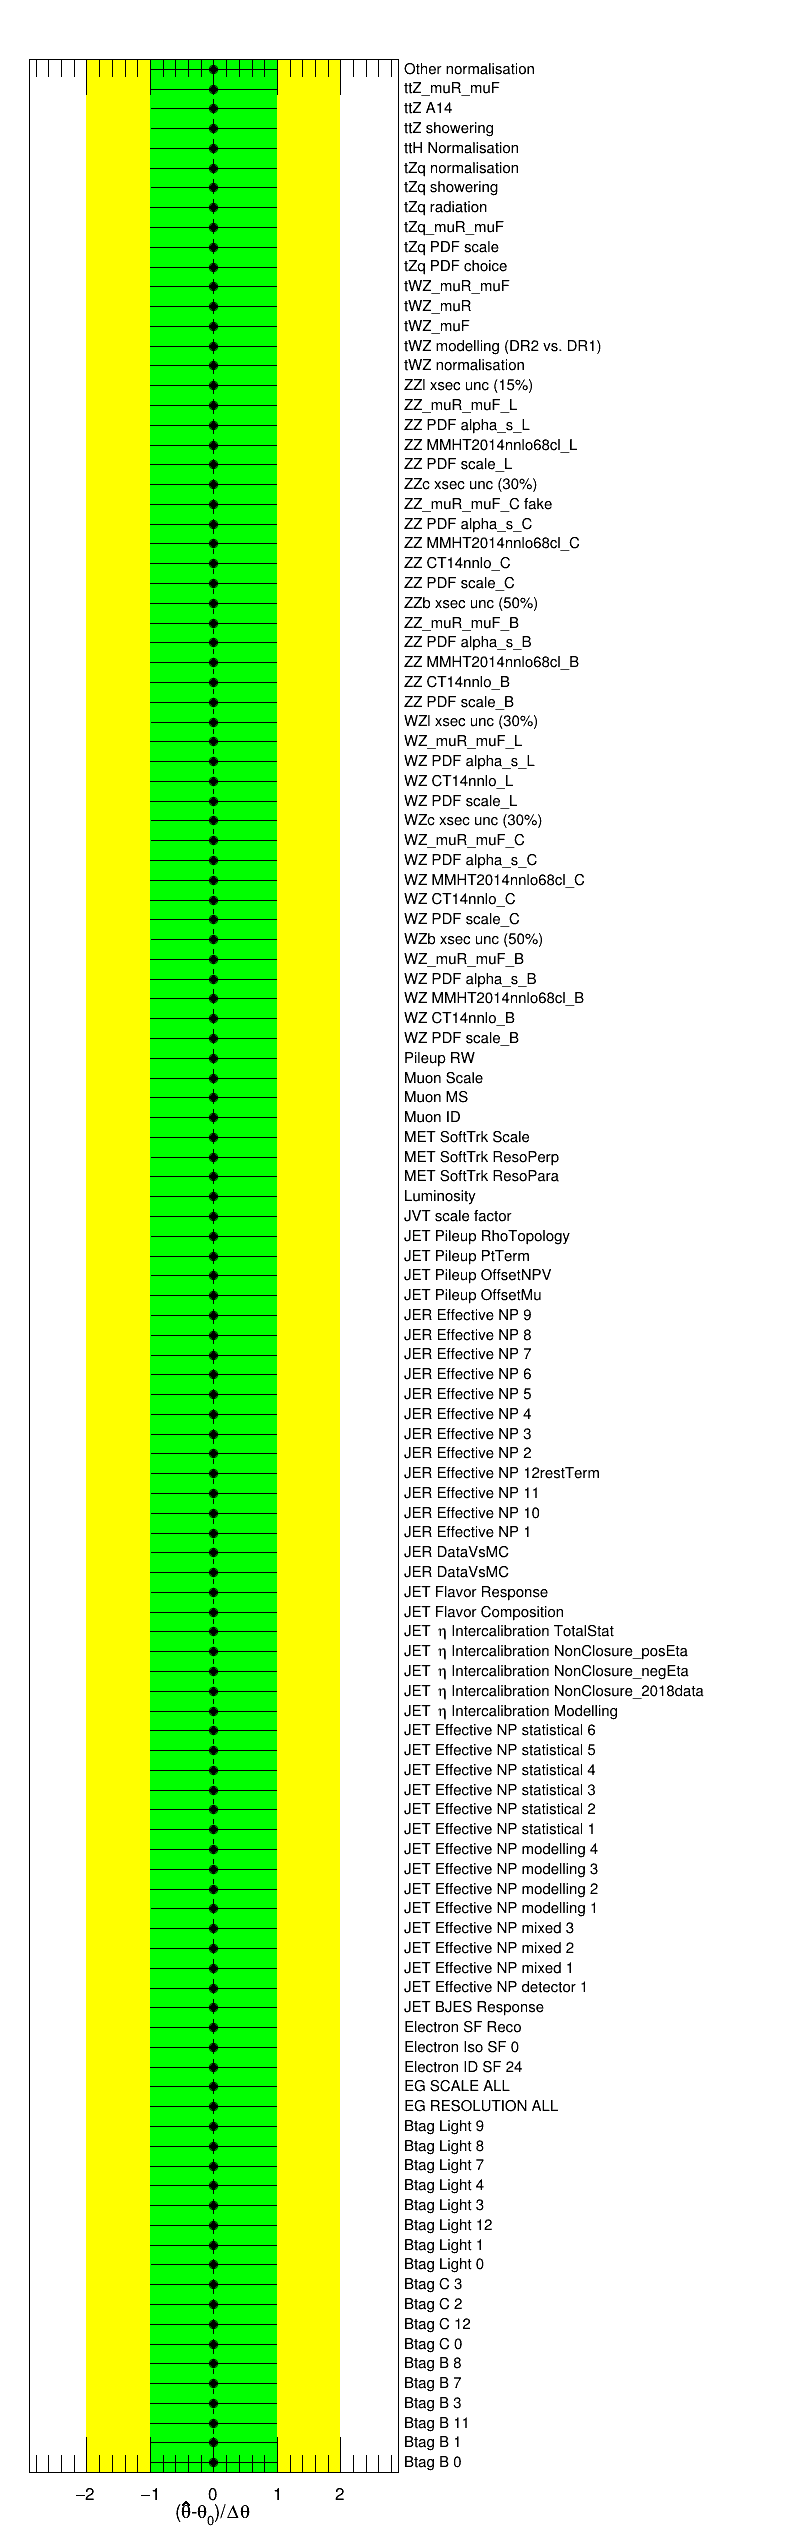
\includegraphics[width=.44\textwidth]{figures/final_config/pullplots/NuisPar.png}
	\caption{Pull plots for the cut and count based (left) and neural network based (right) configuration showing all uncertainties and possible pulls or constraints.}
	\label{fig:PullPlots}
\end{figure}


\chapter{EFT Sensitivity}
\label{ch:eft_sensitivity}
As explained in Section~\ref{sec:theory_ttZ_ttW}, effects from SM-EFT contributions can be investigated by studying off-shell \ttbarZ events. For that, the cross-section ratio and separation power of MC simulations using variations on Wilson coefficients compared to the SM predictions is calculated. Since the operator of interest \optZ is a linear combination of \optB and \optW, as formulated in Equation~\ref{eq:OparatortZ}, cross-section ratios and separation power are calculated for the Wilson coefficients \ctB and \ctW.

\section{Cross-Section Ratio}
\label{sec:CrossSectionRatio}
For the calculation of the cross-section ratio, several distributions for different kinematic variables are used. The set of analysed variables for the \zboson consists of the cosine of the deflection angle \cosstar, the reconstructed mass $m_\text{Z}$ and the transverse momentum $p_{\text{T},\text{Z}}$. For $m_\text{Z}$ and $p_{\text{T},\text{Z}}$ there is an alternative method of reconstruction, which is based on \dR and is indicated by the subscript $\Delta R$. 

The plotted distributions in Figure~\ref{fig:EFTDistributions} show the analysed variations on \ctB and \ctW in the SR-ttZ-NN region for \cosstar. These studies are continued for the all mentioned variables and also for the other regions of the neural network based configuration, resulting in the averaged cross-section ratios which are summarised in Table~\ref{tab:CrossSectionRatio}.

The results show that the highest sensitivity is seen by analysing the variables \cosstar and $m_\text{Z}$. For \ctB, the alternative \dR based variables  show no significant difference to the non-\dR based ones. However, the results for \ctW show noticeable differences between $m_\text{Z}$ and $m_{\text{Z},\Delta R}$. Furthermore, the change in cross-section is higher in variations for the imaginary parts of the Wilson coefficients. This sensitivity to the imaginary part can introduce a non-flat offset, which can be seen in Figure~\ref{fig:EFTDistributions}. It should be noted, that the variations on the real part of \ctW also seem to introduce a non-flat offset.  Since the distribution of the Wilson coefficient variation has non-flat offsets in comparison to the SM prediction, a non-zero separation is expected \cite{shape}.

\begin{table}
	\centering
	\caption{The cross-section ratios calculated for several variations on the Wilson coefficient \ctB (top) and \ctW (bottom), separated into real and imaginary part. All values are averaged over all three regions defined by the neural network based configuration. The highest sensitivities are marked.}
	\vspace{1mm}
	\label{tab:CrossSectionRatio}
	\begin{tabular}{R{23mm}|rrrrr}
		& 
		\multicolumn{1}{l}{\cosstar} & 
		\multicolumn{1}{l}{$m_\text{Z}$} & 
		\multicolumn{1}{l}{$m_{\text{Z},\Delta R}$} & 
		\multicolumn{1}{l}{$p_{\text{T},\text{Z}}$} & 
		\multicolumn{1}{l}{$p_{\text{T},\text{Z},\Delta R}$}\\
		\hline
		ctBRe $+0.3$ 	& $1.00\pm0.00$ & $1.01\pm0.01$ & $1.00\pm0.01$ & $1.00\pm0.01$ & $1.00\pm0.01$ \\
		ctBRe $-0.3$ 	& $1.01\pm0.00$ & $1.01\pm0.01$ & $1.01\pm0.01$ & $1.00\pm0.01$ & $1.00\pm0.01$ \\
		ctBRe $+0.9$ 	& $1.03\pm0.01$ & $1.02\pm0.01$ & $1.02\pm0.01$ & $1.02\pm0.01$ & $1.01\pm0.01$ \\
		ctBRe $-0.9$ 	& $1.04\pm0.01$ & $1.04\pm0.01$ & $1.04\pm0.01$ & $1.03\pm0.01$ & $1.02\pm0.01$ \\
		\hline
		ctBIm $+0.6$ 	& $1.03\pm0.01$ & $1.03\pm0.01$ & $1.03\pm0.01$ & $1.02\pm0.01$ & $1.02\pm0.01$ \\
		ctBIm $-0.6$ 	& $1.02\pm0.01$ & $1.01\pm0.01$ & $1.01\pm0.01$ & $1.01\pm0.01$ & $1.01\pm0.01$ \\
		ctBIm $+1.8$ 	& \cellcolor{highlight}$1.17\pm0.01$ & \cellcolor{highlight}$1.14\pm0.01$ & \cellcolor{highlight}$1.14\pm0.01$ & $1.10\pm0.01$ & $1.09\pm0.01$ \\
		ctBIm $-1.8$ 	& \cellcolor{highlight}$1.17\pm0.01$ & \cellcolor{highlight}$1.14\pm0.01$ & \cellcolor{highlight}$1.14\pm0.01$ & $1.10\pm0.01$ & $1.09\pm0.01$ \\
	\end{tabular}
	
\vspace{3mm}

\begin{tabular}{R{23mm}|rrrrr}
	& 
	\multicolumn{1}{l}{\cosstar} & 
	\multicolumn{1}{l}{$m_\text{Z}$} & 
	\multicolumn{1}{l}{$m_{\text{Z},\Delta R}$} & 
	\multicolumn{1}{l}{$p_{\text{T},\text{Z}}$} & 
	\multicolumn{1}{l}{$p_{\text{T},\text{Z},\Delta R}$}\\
		\hline
		ctWRe $+0.7$ 	& $1.03\pm0.01$ & $1.02\pm0.01$ & $1.02\pm0.01$ & $1.02\pm0.01$ & $1.01\pm0.01$ \\
		ctWRe $-0.7$ 	& $1.03\pm0.01$ & $1.03\pm0.01$ & $1.03\pm0.01$ & $1.02\pm0.01$ & $1.02\pm0.01$ \\
		ctWRe $+1.1$ 	& $1.07\pm0.01$ & $1.04\pm0.01$ & $1.05\pm0.01$ & $1.04\pm0.01$ & $1.04\pm0.01$ \\
		ctWRe $-1.1$ 	& $1.07\pm0.01$ & $1.07\pm0.01$ & $1.06\pm0.01$ & $1.04\pm0.01$ & $1.04\pm0.01$ \\
		\hline
		ctWIm $+0.6$ 	& $1.02\pm0.01$ & $1.02\pm0.01$ & $1.00\pm0.01$ & $1.01\pm0.01$ & $1.01\pm0.01$ \\
		ctWIm $-0.8$ 	& $1.04\pm0.01$ & $1.03\pm0.01$ & $0.99\pm0.01$ & $1.03\pm0.01$ & $1.03\pm0.01$ \\
		ctWIm $+1.2$ 	& \cellcolor{highlight}$1.10\pm0.01$ & $1.08\pm0.01$ & $0.99\pm0.01$ & $1.06\pm0.01$ & $1.06\pm0.01$ \\
		ctWIm $-1.4$ 	& \cellcolor{highlight}$1.13\pm0.01$ & \cellcolor{highlight}$1.10\pm0.01$ & $0.99\pm0.01$ & $1.08\pm0.01$ & $1.08\pm0.01$ \\
	\end{tabular}
\end{table}

\begin{figure}
	\centering
	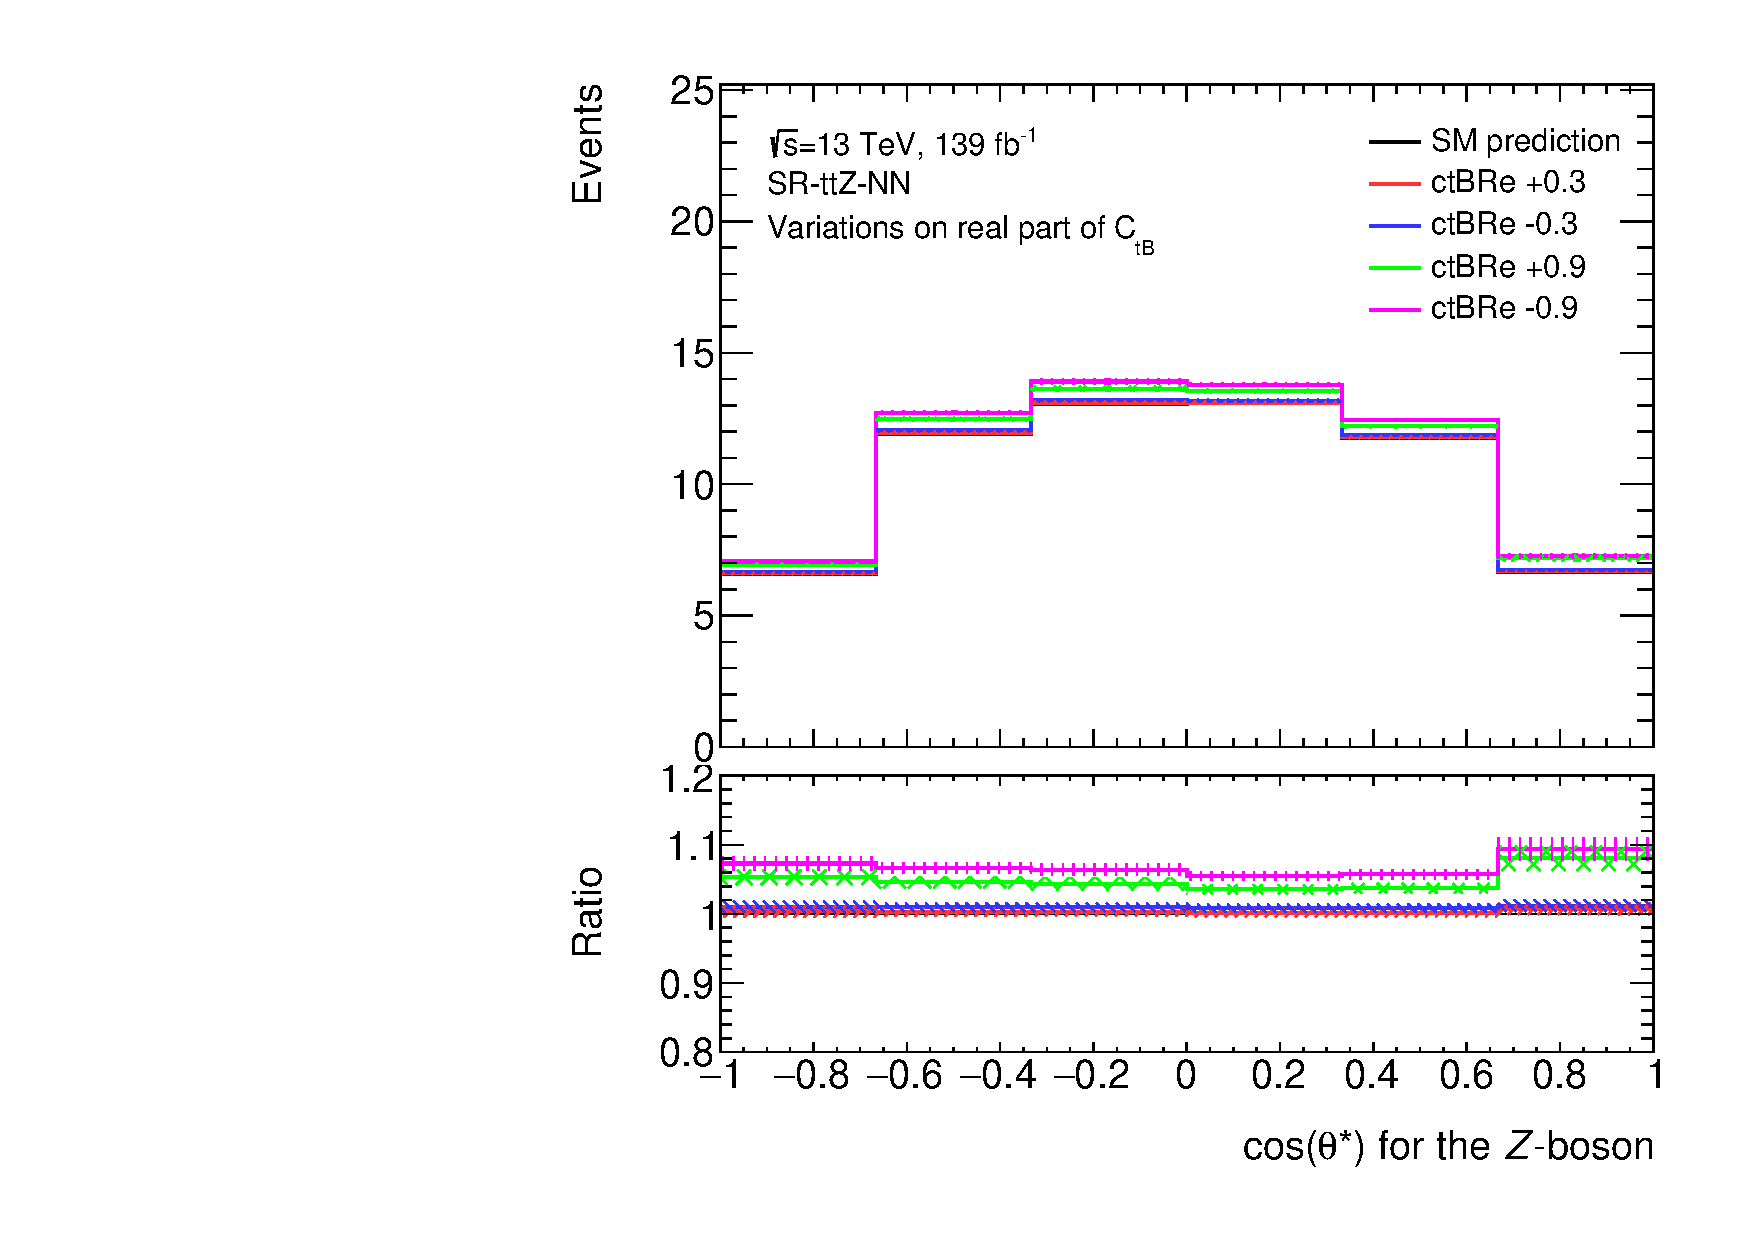
\includegraphics[width=.42\textwidth]{figures/eft/ctBRe/cos_theta_starZ/_cos_theta_starZ_region00_ttZ.pdf}\hspace{8mm}
	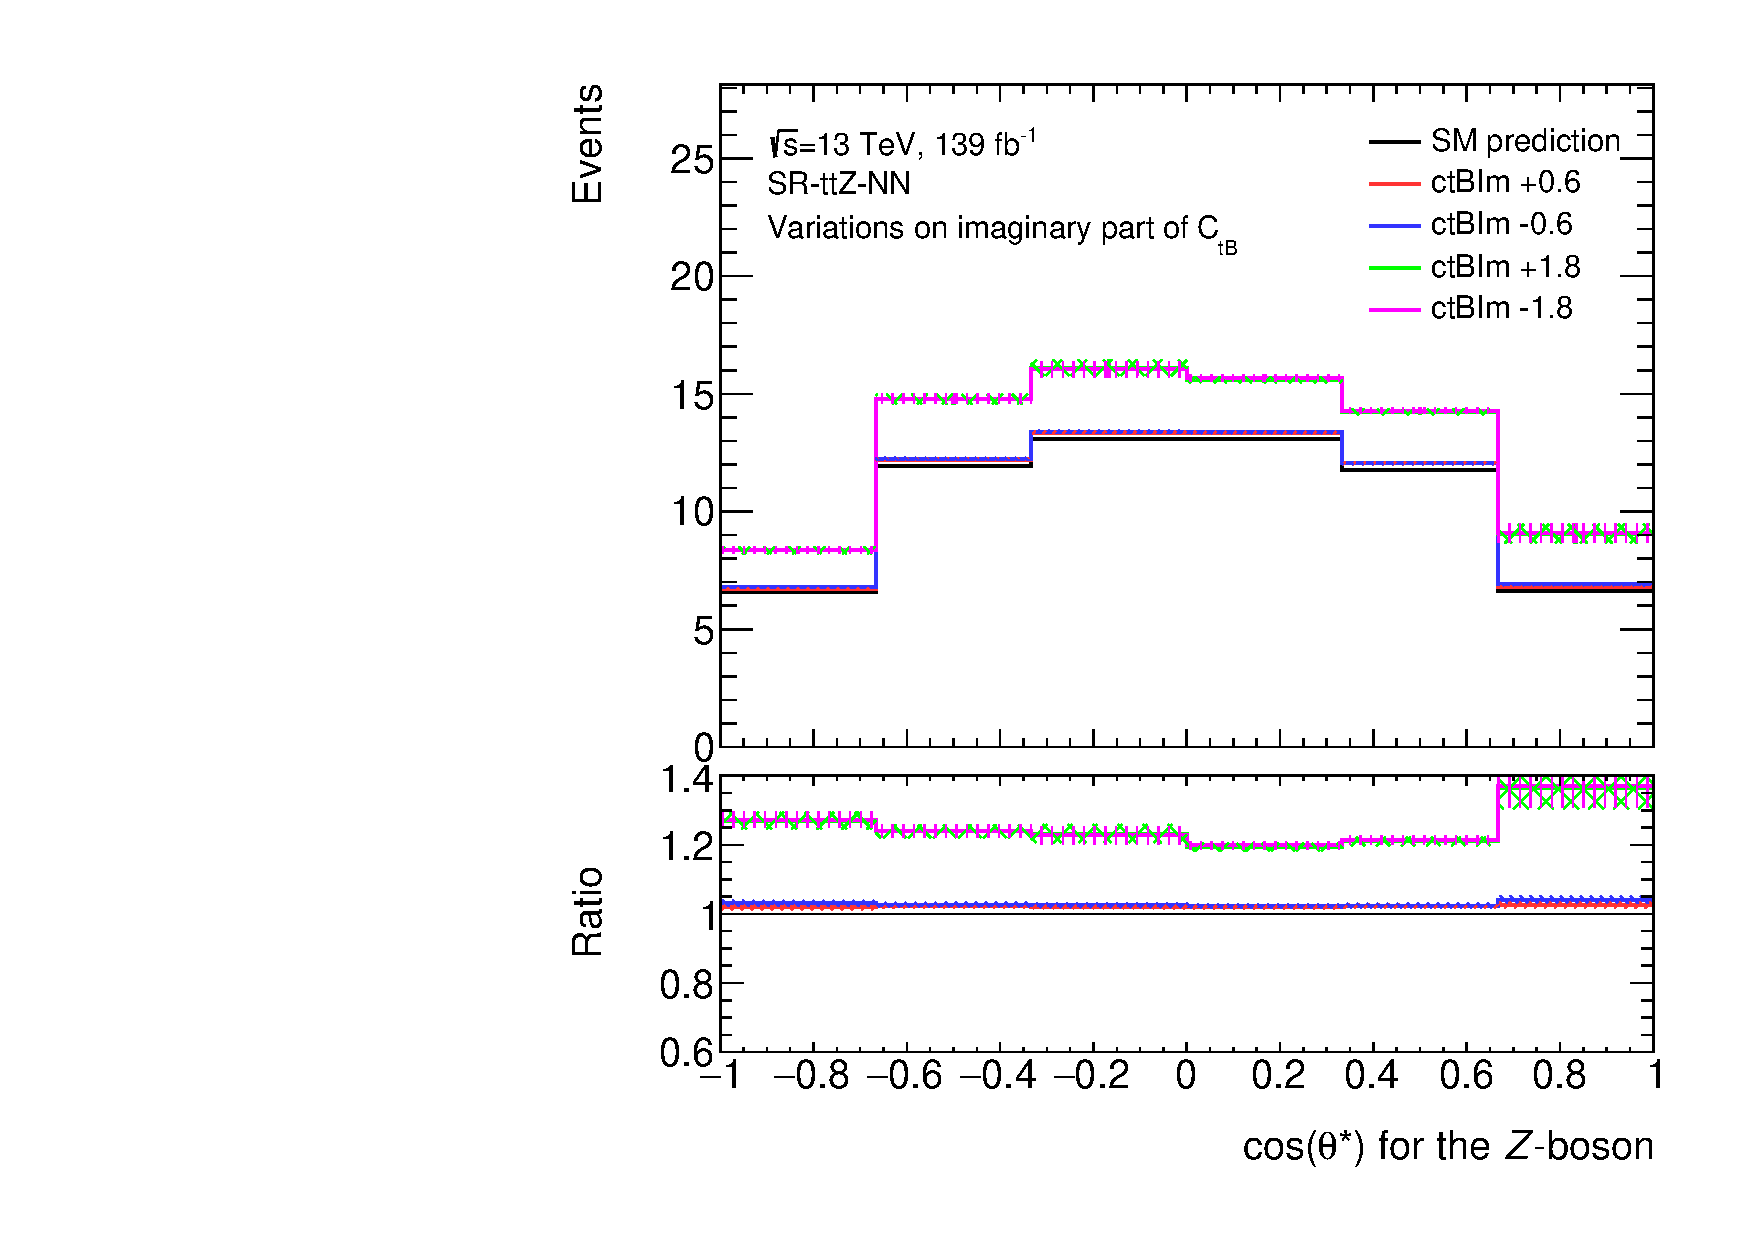
\includegraphics[width=.42\textwidth]{figures/eft/ctBIm/cos_theta_starZ/_cos_theta_starZ_region00_ttZ.pdf}
	
	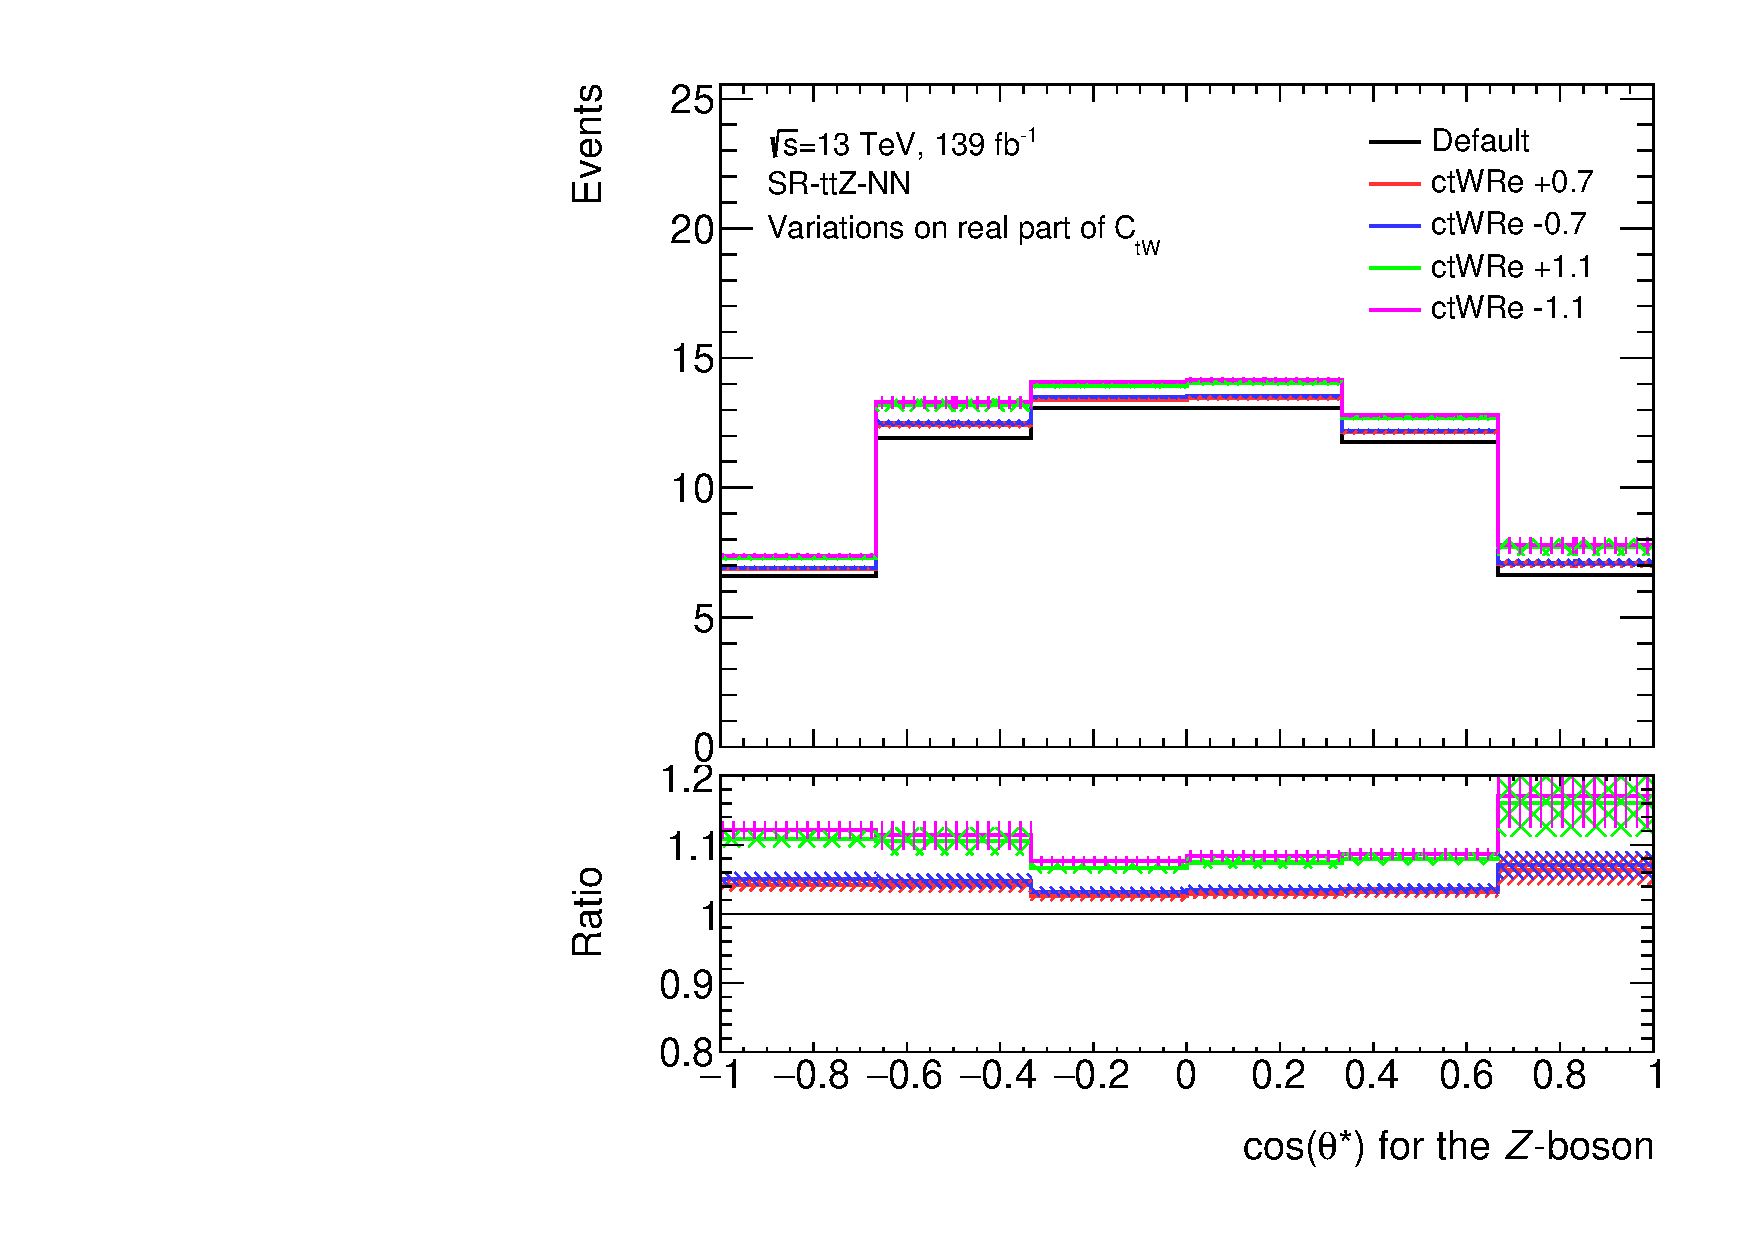
\includegraphics[width=.42\textwidth]{figures/eft/ctWRe/cos_theta_starZ/_cos_theta_starZ_region00_ttZ.pdf}\hspace{8mm}
	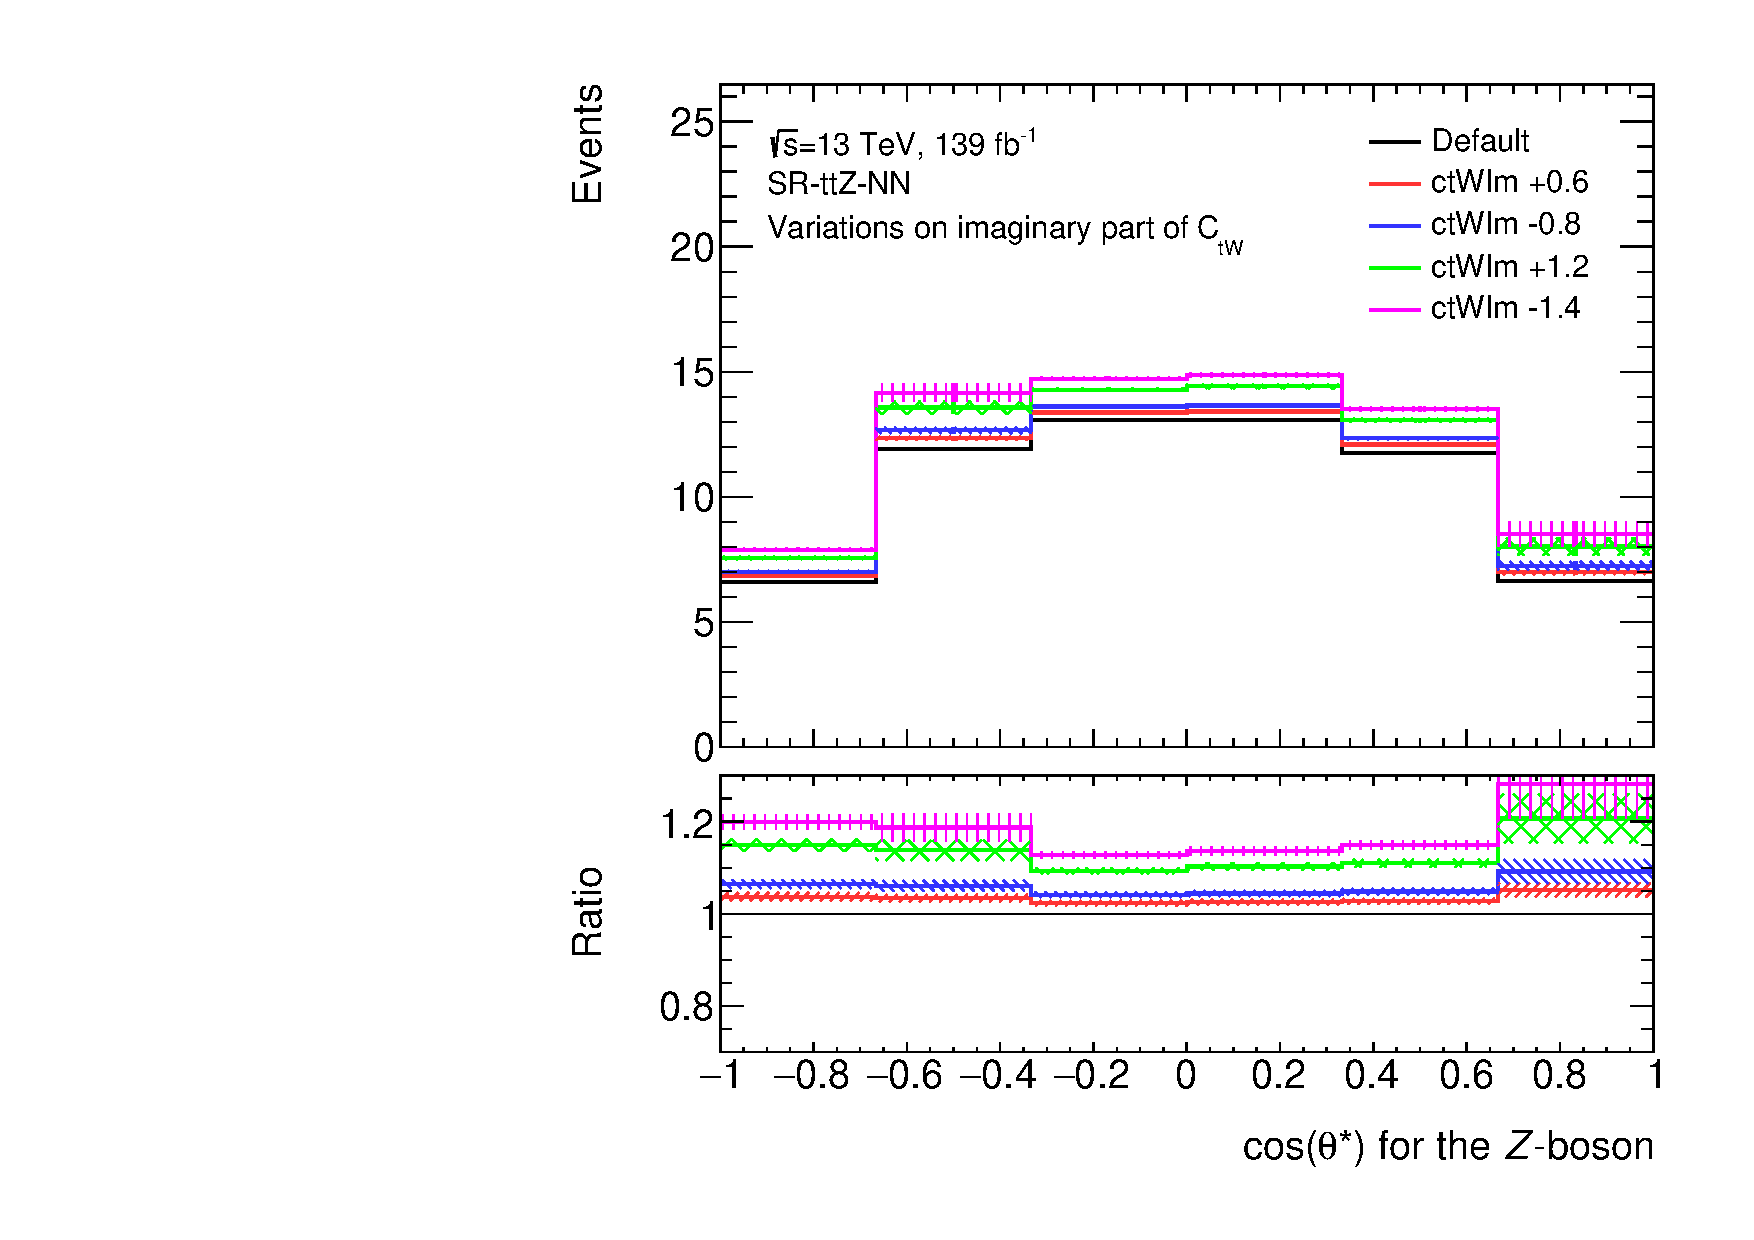
\includegraphics[width=.42\textwidth]{figures/eft/ctWIm/cos_theta_starZ/_cos_theta_starZ_region00_ttZ.pdf}
	\caption{The distribution plots showing several variations on the \ctB (top) and \ctW (bottom) Wilson coefficient plotted against the \cosstar variable in the SR-ttZ-NN region. These are further separated into the real (left) and imaginary (right) part.}
	\label{fig:EFTDistributions}
\end{figure}


\section{Separation Power}
\label{sec:SeparationPower}
The separation power is analysed for both Wilson coefficients, subdivided into the real and imaginary part analogous to the cross-section ratio. The same set of variables is analysed. Using Equation~\ref{eq:SeparationPower} and Gaussian error propagation, the separation power is calculated individually for each region of the neural network based configuration. The averaged separation power for the summed distributions  \ctB are in the order of magnitude of $10^{-4}$--$10^{-7}$ and for \ctW in the order of $10^{-2}$--$10^{-6}$. Both having dominating errors in the order of magnitude of $10^{-1}$--$10^{-2}$.

However, certain regions such as for \cosstar are expected to have a significant separation introduced by the non-flat offset. This prediction can not be supported, since these regions also have high uncertainties due to the low statistics. To further study the separation in these regions, higher statistics are needed. As mentioned in Chapter~\ref{ch:measurements_of_the_inclusive_cross_section}, the High-Luminosity upgrade will provide significantly more data and thus will be useful to this analysis.

%\begin{table}
%	\centering
%	\caption{The separation power calculated for variations on the (Top) real, (Bottom) imaginary part of the Wilson coefficient \ctB.}
%	\label{tab:SeparationPowerCtB}
%	\begin{tabular}{r|lllll}
%		& $\cos(\theta_Z^*)$ & $m_{Z}$ & $m_{Z,\Delta R}$ & $p_{T,Z}$ & $p_{T,Z,\Delta R}$ \\
%		\hline
%		ctBRe $+0.3$ 	& $0.00\pm0.21$ & $0.00\pm0.03$ & $0.00\pm0.03$ & $0.00\pm0.00$ & $0.00\pm0.02$ \\
%		ctBRe $-0.3$ 	& $0.00\pm0.22$ & $0.00\pm0.03$ & $0.00\pm0.03$ & $0.00\pm0.01$ & $0.00\pm0.02$ \\
%		ctBRe $+0.9$ 	& $0.00\pm0.24$ & $0.00\pm0.03$ & $0.00\pm0.03$ & $0.00\pm0.02$ & $0.00\pm0.02$ \\
%		ctBRe $-0.9$ 	& $0.00\pm0.25$ & $0.00\pm0.04$ & $0.00\pm0.04$ & $0.00\pm0.02$ & $0.00\pm0.03$ \\
%	\end{tabular}
%	
%	\vspace{4mm}
%	
%	\begin{tabular}{r|lllll}
%		& $\cos(\theta_Z^*)$ & $m_{Z}$ & $m_{Z,\Delta R}$ & $p_{T,Z}$ & $p_{T,Z,\Delta R}$ \\
%		\hline
%		ctBIm $+0.6$ 	& $0.00\pm0.22$ & $0.00\pm0.03$ & $0.00\pm0.03$ & $0.00\pm0.00$ & $0.00\pm0.03$ \\
%		ctBIm $-0.6$ 	& $0.00\pm0.23$ & $0.00\pm0.02$ & $0.00\pm0.01$ & $0.00\pm0.00$ & $0.00\pm0.02$ \\
%		ctBIm $+1.8$ 	& $0.00\pm0.28$ & $0.01\pm0.03$ & $0.01\pm0.04$ & $0.00\pm0.01$ & $0.00\pm0.04$ \\
%		ctBIm $-1.8$ 	& $0.00\pm0.28$ & $0.01\pm0.03$ & $0.01\pm0.03$ & $0.00\pm0.01$ & $0.00\pm0.04$ \\
%	\end{tabular}
%\end{table}
%
%\begin{table}
%	\centering
%	\caption{The separation power calculated for variations on the (Top) real, (Bottom) imaginary part of the Wilson coefficient \ctW.}
%	\label{tab:SeparationPowerCtW}
%	\begin{tabular}{r|lllll}
%		& $\cos(\theta_Z^*)$ & $m_{Z}$ & $m_{Z,\Delta R}$ & $p_{T,Z}$ & $p_{T,Z,\Delta R}$ \\
%		\hline
%		ctWRe $+0.7$ 	& $0.00\pm0.22$ & $0.00\pm0.03$ & $0.00\pm0.04$ & $0.00\pm0.00$ & $0.00\pm0.03$ \\
%		ctWRe $-0.7$ 	& $0.00\pm0.23$ & $0.00\pm0.02$ & $0.00\pm0.01$ & $0.00\pm0.00$ & $0.00\pm0.02$ \\
%		ctWRe $+1.1$ 	& $0.00\pm0.28$ & $0.01\pm0.03$ & $0.01\pm0.04$ & $0.00\pm0.01$ & $0.00\pm0.04$ \\
%		ctWRe $-1.1$ 	& $0.00\pm0.28$ & $0.01\pm0.03$ & $0.01\pm0.03$ & $0.00\pm0.01$ & $0.00\pm0.04$ \\
%	\end{tabular}
%	
%	\vspace{4mm}
%	
%	\begin{tabular}{r|lllll}
%		& $\cos(\theta_Z^*)$ & $m_{Z}$ & $m_{Z,\Delta R}$ & $p_{T,Z}$ & $p_{T,Z,\Delta R}$ \\
%		\hline
%		ctWIm $+0.6$ 	& $0.00\pm0.24$ & $0.00\pm0.03$ & $0.00\pm0.03$ & $0.00\pm0.00$ & $0.00\pm0.02$ \\
%		ctWIm $-0.8$ 	& $0.00\pm0.25$ & $0.00\pm0.04$ & $0.00\pm0.04$ & $0.00\pm0.00$ & $0.00\pm0.02$ \\
%		ctWIm $+1.2$ 	& $0.00\pm0.26$ & $0.00\pm0.04$ & $0.00\pm0.05$ & $0.00\pm0.01$ & $0.00\pm0.03$ \\
%		ctWIm $-1.4$ 	& $0.00\pm0.27$ & $0.00\pm0.05$ & $0.00\pm0.05$ & $0.00\pm0.01$ & $0.00\pm0.03$ \\
%	\end{tabular}
%\end{table}

\chapter{Conclusion}
\label{ch:conclusion}
To conclude this thesis, a brief summary and possible improvements for future studies are presented.

This study analysed the simultaneous measurements of \ttbarZ and \ttbarW events in off-shell regions. This was done by defining sensitive regions, which were then used in the fitting process of the inclusive cross-section. Additionally, this study further separated the fakes background, which is dominating in the trileptonic decay channel. 

The region definition used two different approaches, as described in Chapter~\ref{ch:region_definition}, to define a signal region for \ttbarZ and two control regions for \ttbarW and fakes. The cut and count based configuration is based on manually set cuts on \ETMiss and \dR, which were studied and optimised. For the neural network based configuration a DNN was trained to identify \ttbarZ, \ttbarW and fakes events by using several variables as inputs. This DNN defined class scores for each process, which were then used to define the three regions. The comparison of both approaches showed that the DNN based regions are cleaner in comparison to the cut and count based regions. However, the number of events in the NN based signal region decreased by $44\%$, which is problematic for the analysis, because the off-shell region provides low statistics. These results were reflected in the fitting process.

A binned likelihood fit was conducted including one PoI for the signal strength $\mu_{t\bar{t}Z}$ and two PoI for the normalisation of \ttbarW and fakes as well as several NP for the uncertainties. As expected from the region definition, the uncertainties for the normalisation factors decreased using the NN based configuration. For $N_{t\bar{t}W}$ the uncertainties decreased by $37\%$, for $N_\text{Fakes}$ by $6\%$, whereby the uncertainties on $\mu_{t\bar{t}Z}$ increased by $2\%$. 

Thus, for studies in the off-shell region, where \ttbarZ or \ttbarW events are analysed, it is recommended to use a neural network based region definition, as it improves the overall results and especially the of the different processes. The improvements in the normalisation are expected to outweigh the increased uncertainty of the signal strength. 

As discussed before, in Chapter~\ref{ch:measurements_of_the_inclusive_cross_section}, the most impactful improvement is expected to be the usage of a greater dataset, since the statistical uncertainty is higher than the systematic uncertainty for all PoI. Further improvements could be achieved by modifying the used DNN framework to allow the sum of variables to be used as input. By studying the chosen cuts for the NN based configuration in more detail, including non-linear cuts, additional improvements could be realised.

Furthermore, the SM-EFT sensitivity was analysed in Chapter~\ref{ch:eft_sensitivity} by comparing the SM-prediction to several samples which include variations on Wilson coefficients. For the comparison, the cross-section ratios and the separation power was calculated for several variables. The results of the cross-section ratio showed that the studied variables have higher sensitivity to the imaginary parts of the analysed variations. The separation power provided no further information because of the dominating uncertainties due to the low amount of events.

As for the fitting results, a greater dataset is expected to reduce the uncertainties and allow for more precise calculations. Furthermore, to increase the sensitivity to possible EFT contributions further, a separation into high-$Z$-mass and low-$Z$-mass regions could be useful. This, as mentioned in Section~\ref{sec:theory_ttZ_ttW}, is due to the SM-EFT contributions increase for higher boson masses.
\clearpage

\appendix
\bibliography{bthesis_raschke_datenbank} 
%
%\chapter{Appendix Figures}
%\begin{figure}
%	\centering
%	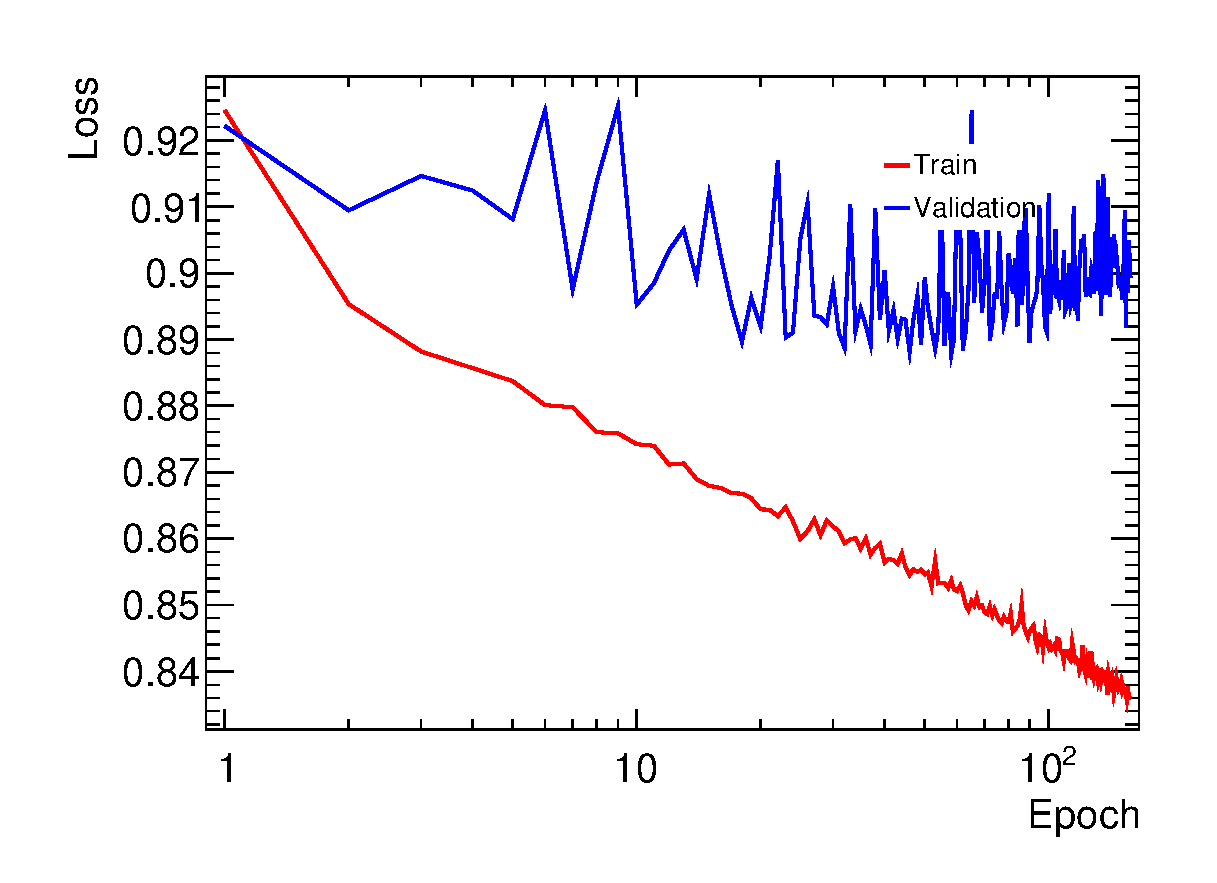
\includegraphics[width=.47\textwidth]{figures/neural_networks/output/MyModel_0_loss.eps}\hspace{8mm}
%	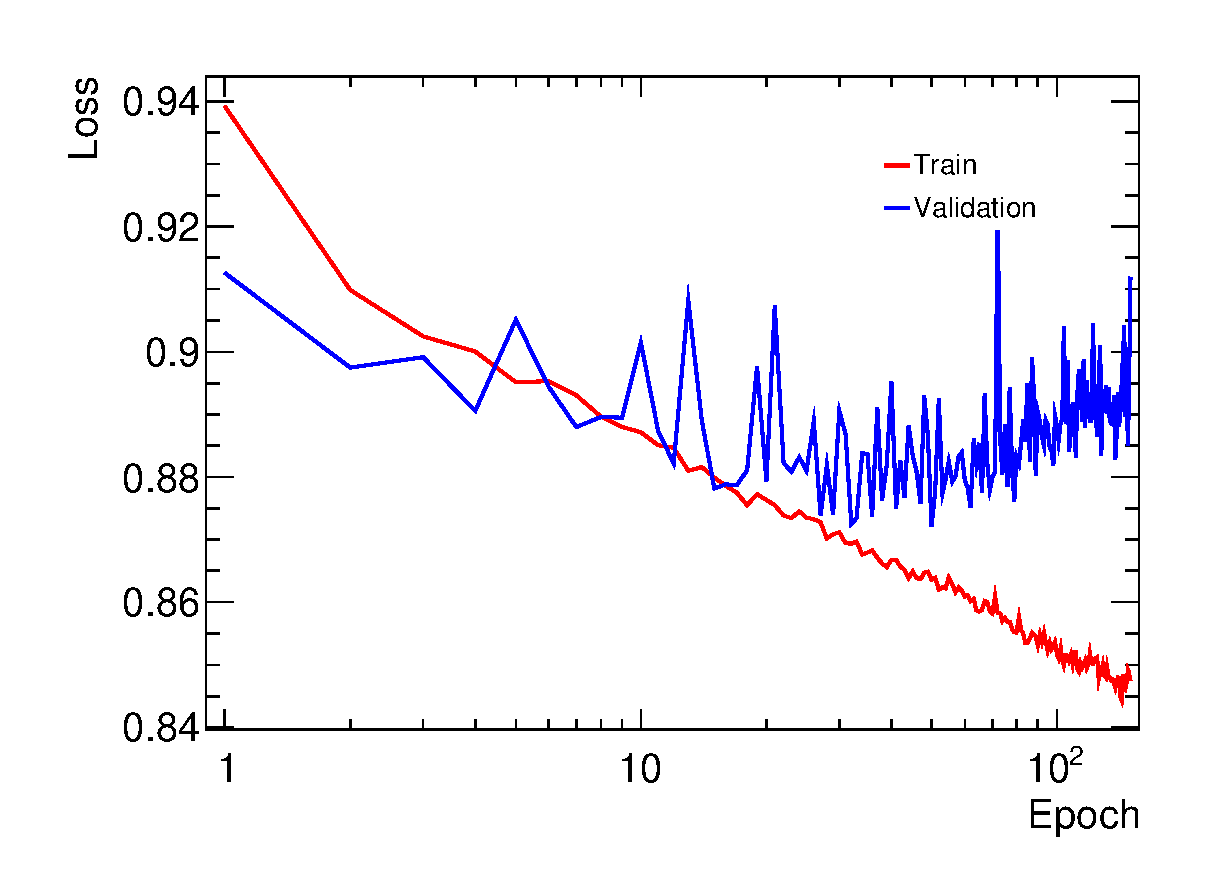
\includegraphics[width=.47\textwidth]{figures/neural_networks/output/MyModel_1_loss.eps}
%	\caption{The loss function for (left) first and (right) second fold. The training was stopped early at 150 epochs. }
%	\label{fig:Epochs}
%\end{figure}
%\begin{figure}
%	\centering
%	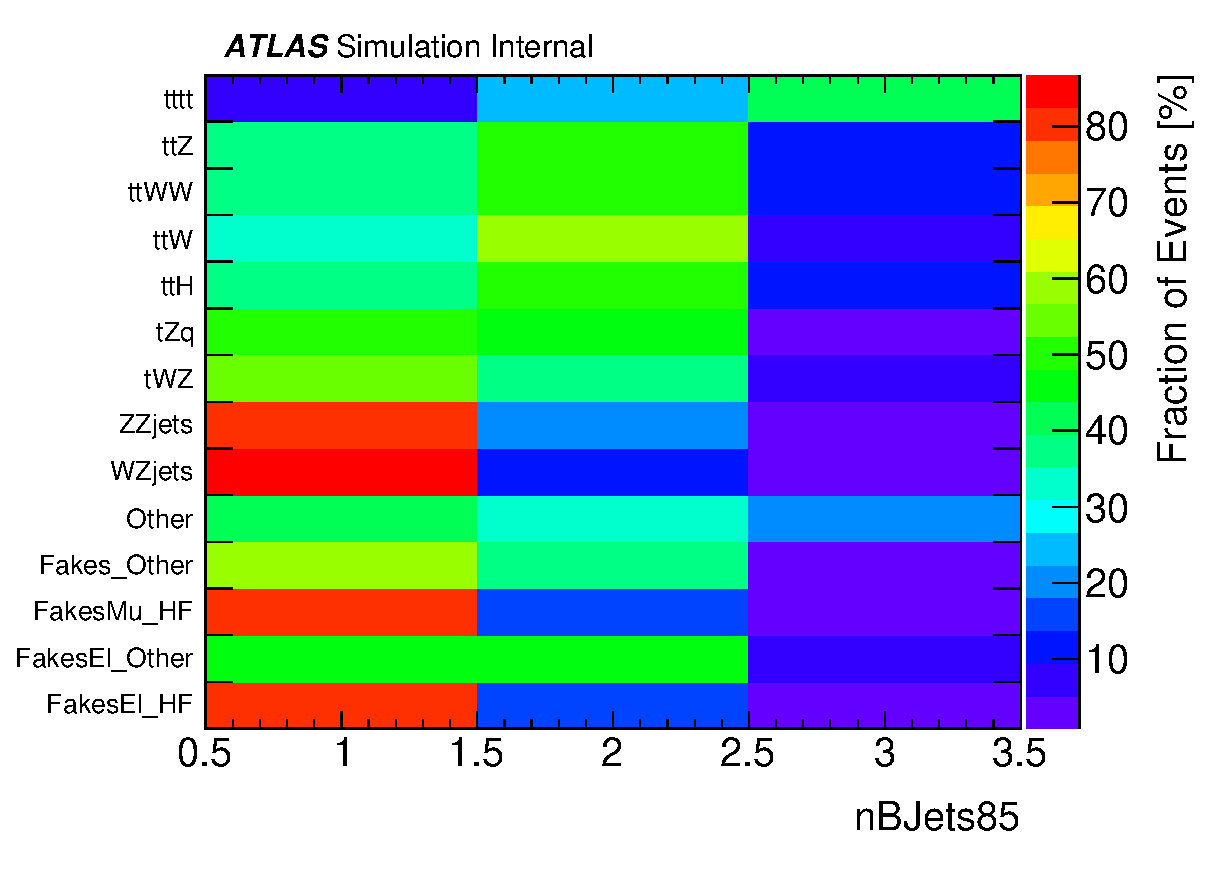
\includegraphics[width=.4\textwidth]{figures/neural_networks/input/2DSeparation_nBJets85.eps}\hspace{8mm}
%	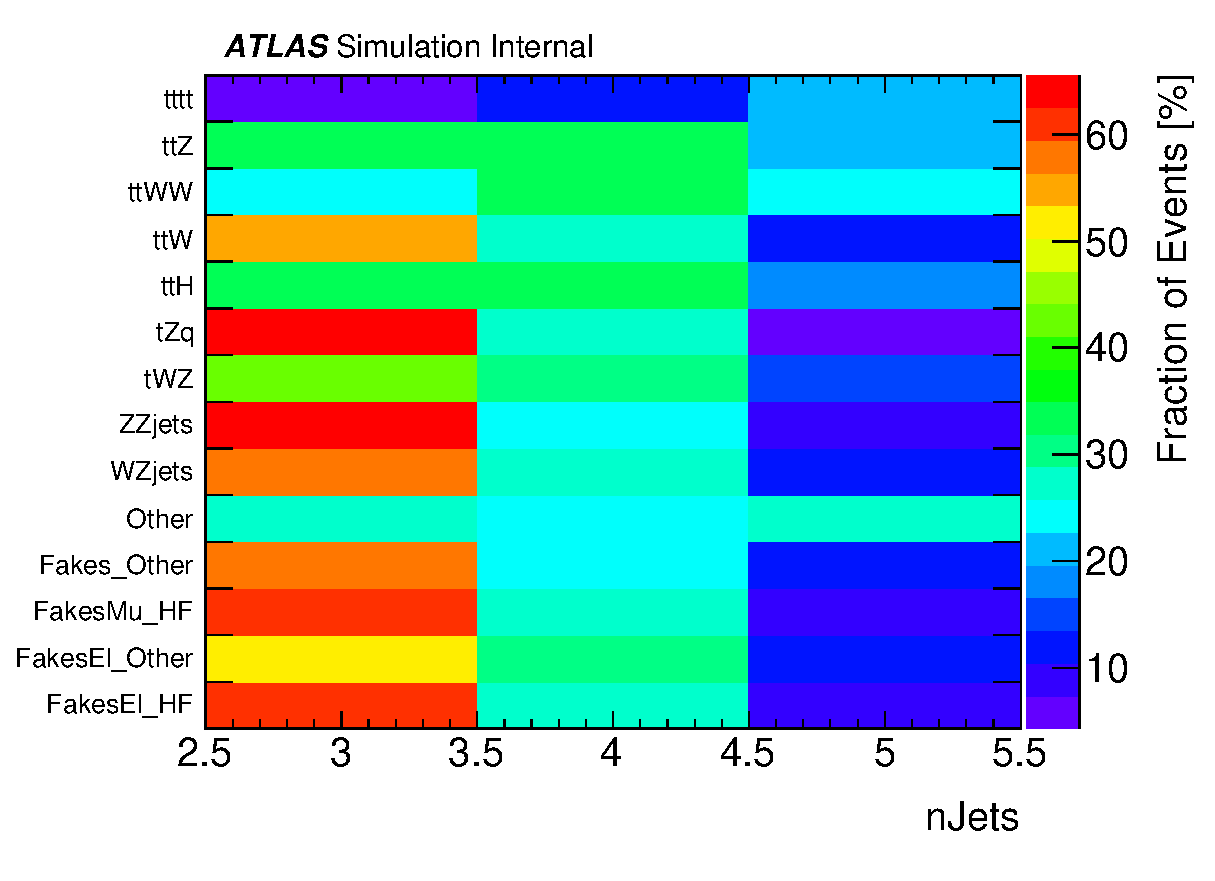
\includegraphics[width=.4\textwidth]{figures/neural_networks/input/2DSeparation_nJets.eps}
%	
%	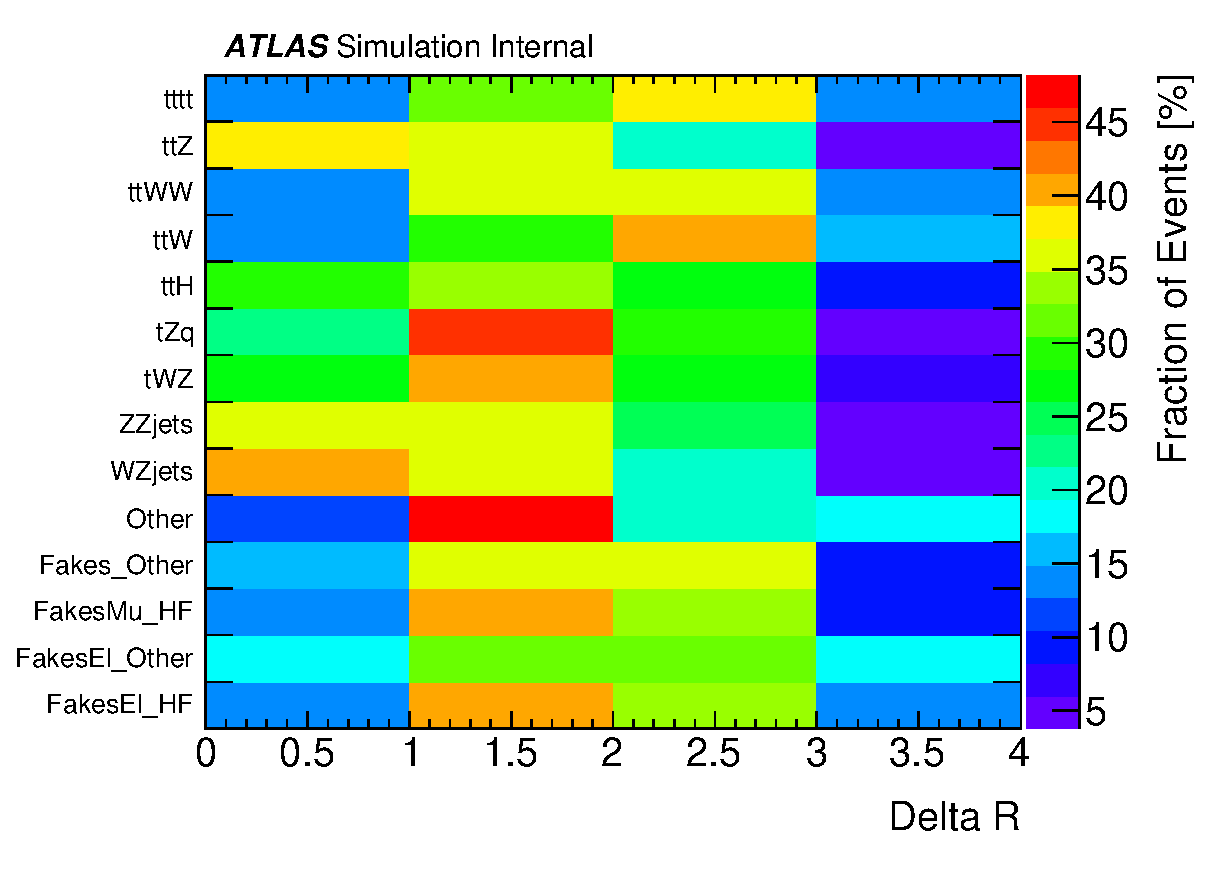
\includegraphics[width=.4\textwidth]{figures/neural_networks/input/2DSeparation_dRllz1_dR.eps}\hspace{8mm}
%	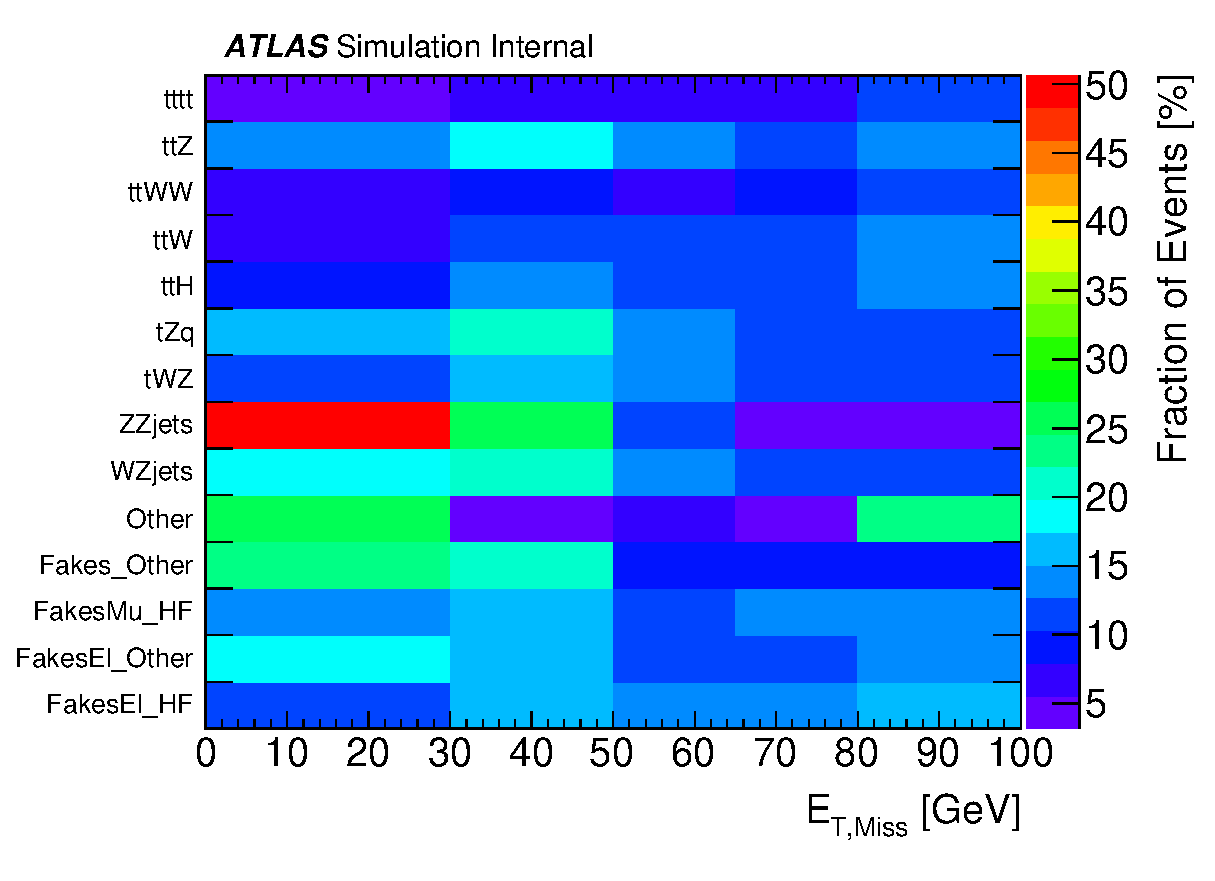
\includegraphics[width=.4\textwidth]{figures/neural_networks/input/2DSeparation_eT_miss.eps}
%	
%	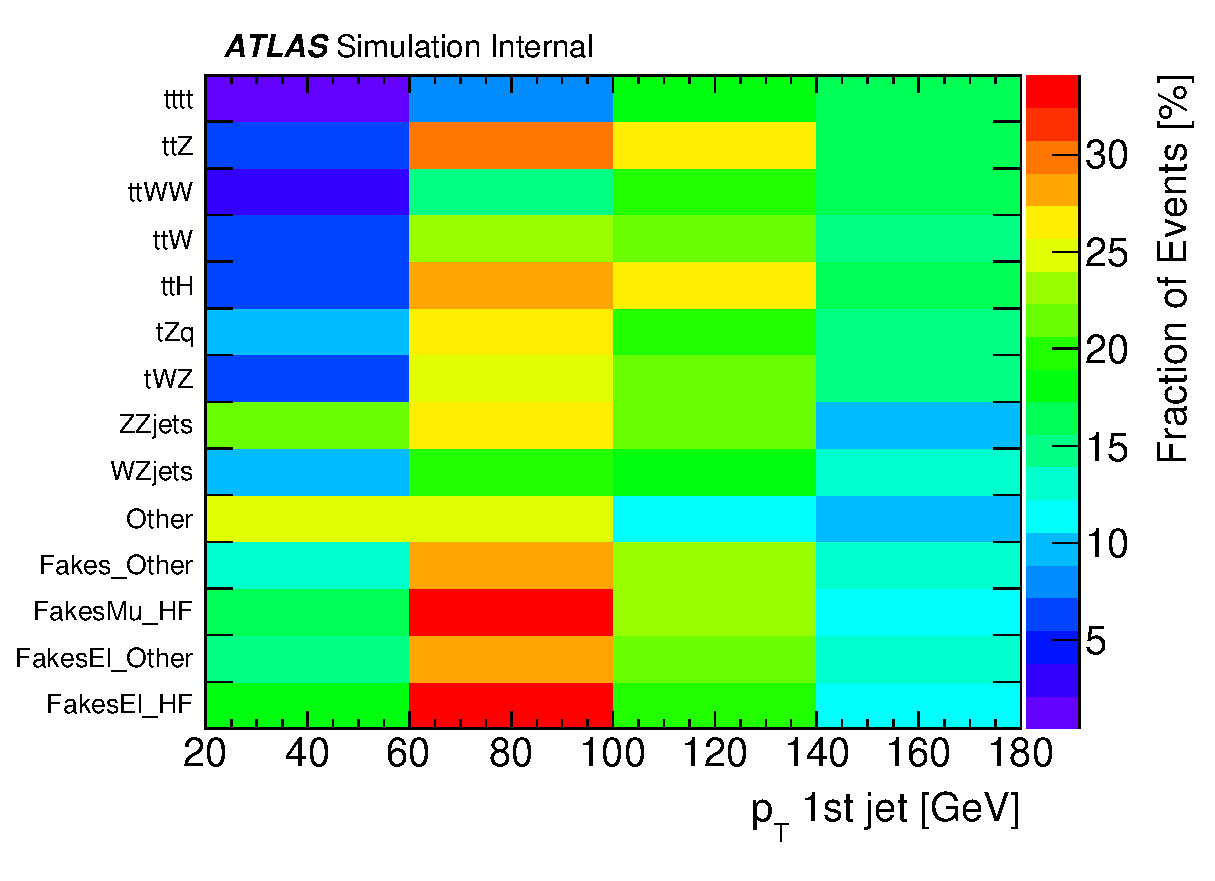
\includegraphics[width=.4\textwidth]{figures/neural_networks/input/2DSeparation_pT_1jet.eps}\hspace{8mm}
%	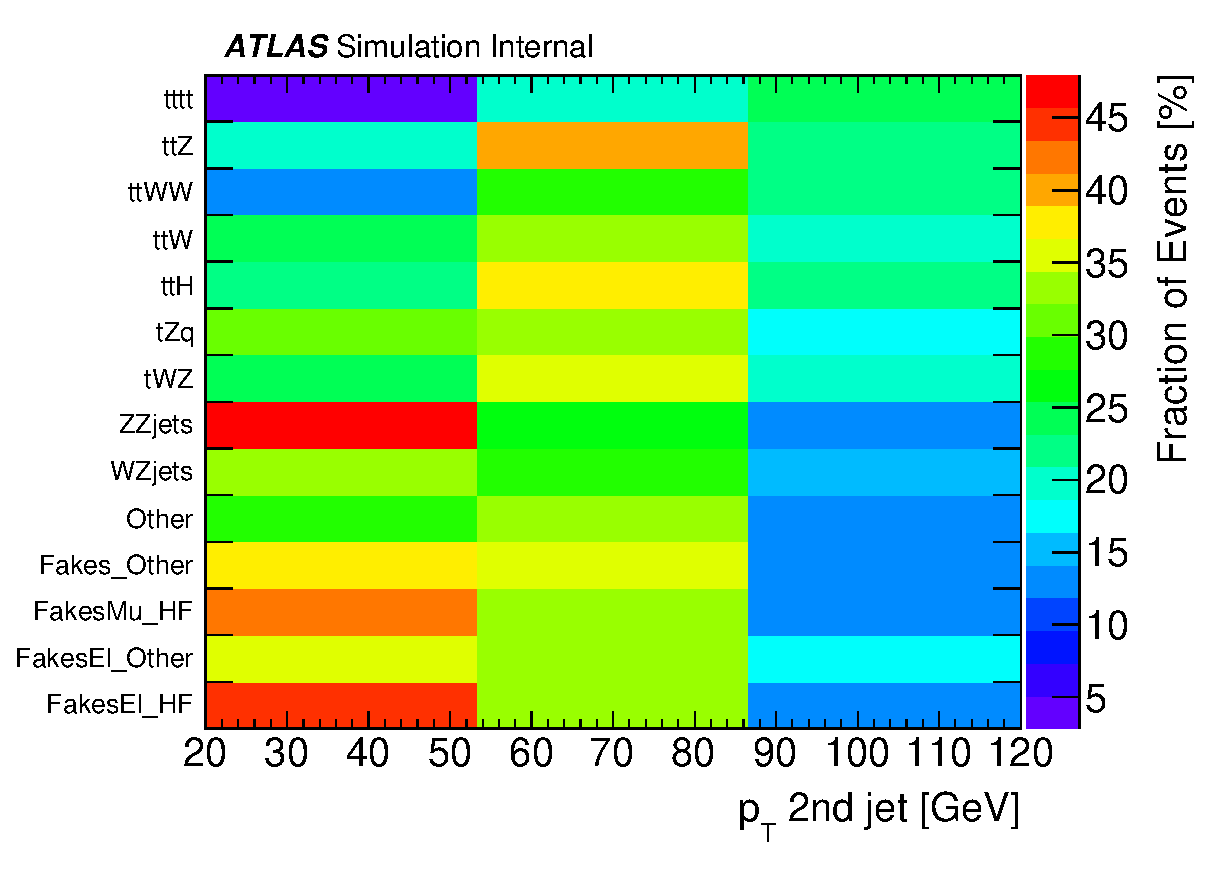
\includegraphics[width=.4\textwidth]{figures/neural_networks/input/2DSeparation_pT_2jet.eps}
%	
%	\includegraphics[width=.4\textwidth]{figures/neural_networks/input/2DSeparation_pT_3jet.eps}\hspace{8mm}
%	\includegraphics[width=.4\textwidth]{figures/neural_networks/input/2DSeparation_pT_1lep.eps}
%	
%	\includegraphics[width=.4\textwidth]{figures/neural_networks/input/2DSeparation_pT_2lep.eps}\hspace{8mm}
%	\includegraphics[width=.4\textwidth]{figures/neural_networks/input/2DSeparation_pT_3lep.eps}
%	
%	\caption{2D separation plots for the used input variables in the DNN.}
%	\label{fig:nn_inputvariables}
%\end{figure}
%
%\begin{figure}
%	\centering
%	\includegraphics[width=.47\textwidth]{figures/neural_networks/output/TrainTest_MyModel_Classification-DNNttZ_0.eps}\hspace{8mm}
%	\includegraphics[width=.47\textwidth]{figures/neural_networks/output/TrainTest_MyModel_Classification-DNNttZ_1.eps}
%	
%	\includegraphics[width=.47\textwidth]{figures/neural_networks/output/TrainTest_MyModel_Classification-DNNttW_0.eps}\hspace{8mm}
%	\includegraphics[width=.47\textwidth]{figures/neural_networks/output/TrainTest_MyModel_Classification-DNNttW_1.eps}
%	
%	\includegraphics[width=.47\textwidth]{figures/neural_networks/output/TrainTest_MyModel_Classification-DNNFakes_0.eps}\hspace{8mm}
%	\includegraphics[width=.47\textwidth]{figures/neural_networks/output/TrainTest_MyModel_Classification-DNNFakes_1.eps}
%	\caption{Separation plots showing signal against background for (top) \ttbarZ, (centre) \ttbarW, (bottom) fakes class.}
%	\label{fig:nn_OutputSeparation}
%\end{figure}
%
%
%\clearpage
%\begin{figure}
%	\centering
%	\includegraphics[width=.4\textwidth]{figures/initial_config/distribution/region1.png}\hspace{8mm}
%	\includegraphics[width=.4\textwidth]{figures/initial_config/distribution/region1_postFit.png}
%	
%	\includegraphics[width=.4\textwidth]{figures/initial_config/distribution/region2.png}\hspace{8mm}
%	\includegraphics[width=.4\textwidth]{figures/initial_config/distribution/region2_postFit.png}
%	
%	\includegraphics[width=.4\textwidth]{figures/initial_config/distribution/region3.png}\hspace{8mm}
%	\includegraphics[width=.4\textwidth]{figures/initial_config/distribution/region3_postFit.png}
%	
%	\caption{The (left) pre-fit, (right) post-fit distributions of the DNN \ttbarZ score for the cut and count based regions.}
%	\label{fig:InitialPreFitPostFitPlots}
%\end{figure}
%
%\clearpage
%\begin{figure}
%	\centering
%	\includegraphics[width=.4\textwidth]{figures/final_config/distribution/SR-offZ-ttZ.png}\hspace{8mm}
%	\includegraphics[width=.4\textwidth]{figures/final_config/distribution/SR-offZ-ttZ_postFit.png}
%	
%	\includegraphics[width=.4\textwidth]{figures/final_config/distribution/CR-offZ-ttW.png}\hspace{8mm}
%	\includegraphics[width=.4\textwidth]{figures/final_config/distribution/CR-offZ-ttW_postFit.png}
%	
%	\includegraphics[width=.4\textwidth]{figures/final_config/distribution/CR-offZ-Fakes.png}\hspace{8mm}
%	\includegraphics[width=.4\textwidth]{figures/final_config/distribution/CR-offZ-Fakes_postFit.png}
%	
%	\caption{The (left) pre-fit, (right) post-fit distributions of the DNN \ttbarZ score for neural network based regions.}
%	\label{fig:FinalPreFitPostFitPlots}
%\end{figure}


\begin{otherlanguage}{ngerman}
\Declaration

\begin{figure}[H]
	\centering
	\vspace{-10mm}
	
	\hspace{27mm}\includegraphics[width=.4\textwidth]{sign.png}	
\end{figure}
\end{otherlanguage}
\end{document}

